%
% This template has been created by:
%   Pascal Bercher, 
%   - pascal.bercher@anu.edu.au, 
%   - https://bercher.net
%
% The newest version can be found on:
% https://gitlab.anu.edu.au/u1092535/latex-templates/
%
% Version number: 
%   At least 1.10 (18.5.2025), but maybe newer, as I might forgotten 
%   to update the version number here. Please look up the current
%.  version in the file readme-and-changelog.txt.
%
% Version history:
%   Detailed change logs are provided in the file readme-and-changelog.txt
%
% I was too lazy to put it under a specific license (will do
% so eventually; but might take me a few more years...), but
% you are still free to use and alter it. However, since I 
% put a *lot* of effort (and experience) in it, I insist on
% keeping my credentials in here (at the top), which give
% credit to me as an author. I explicitly forbid re-publishing
% my code (or content) until I put it under a specific license
% which would then clarify the rights. However, as said, *using*
% it is *of course* allowed, this is after all why I created it!
%
% Good luck with your thesis, and enjoy the journey  --  Pascal

\documentclass[a4paper,twoside,cleardoublepage=plain,bibliography=totoc]{scrbook}

\usepackage[a4paper]{geometry}                    % used for defining the title page

\usepackage{xurl}                                 % allows long URLs to break at any position

\usepackage[standardsections]{scrhack}                % fixes an error causes by loading titlesec for class scrbook

\usepackage{titlesec}                                % used to add those horizontal lines around chapter package; see defs below.

\usepackage[backref=page]{hyperref}               % defines style of references / links
\hypersetup{
linktocpage,                                      % in the table of contents, the numbers serve as links, not the entries
colorlinks  = true,                               % the items are colored instead of colored boxes around them
urlcolor    = cyan,
linkcolor   = red,
citecolor   = blue
}
% the following makes back references more appealing.
% Taken from: https://tex.stackexchange.com/questions/183702/formatting-back-references-in-bibliography-bibtex
\renewcommand*{\backref}[1]{}
\renewcommand*{\backrefalt}[4]{[%
\ifcase #1 Not cited.%
  \or Cited on page~#2.%
  \else Cited on pages #2.%
\fi]}


% Ensure proper font/input encodings for accented characters (e.g., \k{})
\usepackage[T1]{fontenc}
\usepackage[utf8]{inputenc}
\usepackage{lmodern}
\usepackage{listings}
\usepackage{algorithmic}                            % algorithmic environment for pseudocode

\usepackage{datetime}                                % to be able to print month & year on title page
\newdateformat{monthonly}{\monthname[\THEMONTH]}
\usepackage{amssymb,amsthm,amsmath}                  % standard math packages; often used
\usepackage{graphicx}                                % allows including graphics
\usepackage[numbers,sort&compress]{natbib}
                                  % a specific citation style
\usepackage{floatrow}                                % allows to place a caption next to a figure
\floatsetup[table]{capposition=top}                 % forces table captions to appear on top.
\usepackage[linesnumbered,ruled,vlined]{algorithm2e} % used for depicting algorithms
\usepackage{booktabs}                                % for tables that actually look nice!
\usepackage{paralist}                                % provides compactitem, a more compact itemize
\usepackage{parskip}                                 % when this is included, no indentations are used for new paragraphs,
\usepackage{xspace}                                  % smart space after macros used in text
                                                 % and instead paragraphs are separated by a small distance between them
\usepackage{tikz}
\usepackage{xcolor}

\usetikzlibrary{shapes,arrows,positioning}

% [requires titlesec]
% Surrounds all chapter titles by lines,
\titleformat{\chapter}[display]
{\bfseries\huge}
{\filleft\Large\chaptertitlename~\thechapter}
{3ex}
{\titlerule\vspace{1.5ex}\filright}
[\vspace{1ex}\titlerule]

% fixes a compilation error that otherwise occurs in combination with scrbook
% see https://tex.stackexchange.com/questions/625083/adding-horizontal-line-before-and-after-chapter-heading-in-scrbook
% \titleformat{\section}
%  {\normalfont\Large\bfseries}{\thesection}{1em}{}
% \titleformat{\subsection}
%  {\normalfont\large\bfseries}{\thesubsection}{1em}{}
% \titleformat{\subsubsection}
%  {\normalfont\normalsize\bfseries}{\thesubsubsection}{1em}{}
% EDIT: mid 2025, we found out that this "fix" doesn't actually work. Also, there is no compilation error! :)
%       So, it is unclear what this is even about... I guess it can be deleted, but I'll leave it for later
%.      investigation. (I'm planning to resolve the warning regarding not to use the KOMA script.)
 

 % EasyCrypt code style
\lstdefinestyle{easycrypt}{
    language=ML,
    basicstyle=\ttfamily\small,
    keywordstyle=\color{blue}\bfseries,
    commentstyle=\color{green!60!black},
    stringstyle=\color{red},
    numbers=left,
    numberstyle=\tiny\color{gray},
    stepnumber=1,
    numbersep=5pt,
    backgroundcolor=\color{gray!10},
    showspaces=false,
    showstringspaces=false,
    showtabs=false,
    frame=single,
    rulecolor=\color{black},
    tabsize=2,
    captionpos=b,
    breaklines=true,
    breakatwhitespace=false,
    escapeinside={\%*}{*)}
}


\lstset{
    breaklines=true,
    breakatwhitespace=true,
    frame=single,
    keepspaces=true,
    aboveskip=\baselineskip,
    belowskip=\baselineskip,
    breakindent=0pt
}

% Set your individual data for the title page in the configuration file
% AND DON'T SCREW UP THIS DATA! You should know, for example, whether it's
% an Honours thesis or not, or in which semester it is running.

% Set your name:
%  (Well, your name.)
\newcommand{\AuthorName} {Xiuchen Gu}


% Set the title of your work:
%  (Choose an informative and interesting title.)
\newcommand{\ProjectTitle} {Formal Verification of ElGamal-based KEM IND-CCA1 Security and q-DDH Equivalence in EasyCrypt}


% Set which titlepage layout you prefer. Both provide the exact same
% information, they only differ in design to give you a bit of individuality
%  (change second line accordingly)
\newif\ifStandardTitle % do not delete this part!
\StandardTitletrue     % comment out (or use \StandardTitlefalse)
                       % to switch to an alternative title page layout


% Set the name of your school:
%  (School of Computing, School of Engineering,
%   or School of Cybernetics)
\newcommand{\School} {School of Computing}


% Set the name of your college:
%  (However your College is called.)
\newcommand{\College} {College of Systems and Society}


% Set your project points:
%  (6 or 12)
%  can be ignored for Honours theses, since those are always 24 pt anyway
%  and hence set automatically
\newcommand{\ProjectPoints} {6}


% Set whether it's an Honours thesis:
%  (change second line accordingly)
\newif\ifHonoursThesis % do not delete this part!
\HonoursThesistrue     % or \HonoursThesisfalse or comment out


% Set your semester:
%  (S1 or S2 or S1/S2 or S2/S1 or Summer)
\newcommand{\Semester} {S2}


% Set your year:
%  (YYYY or YYYY--YYYY in case of S2/S1)
\newcommand{\Year} {2025}


% Set your degree:
%  (Whatever your degree is called.)
%  (Only required if Honours = true)
\newcommand{\Degree} {Bachelor of Advanced Computing}


% Set your course code and name:
%  (Whatever your course code and name is.)
%  (Only required if Honours = false)
\newcommand{\CourseCode} {COMP1234}
\newcommand{\CourseName} {Course Name}


% Set name of first supervisor:
%   (Whatever her or his name is.)
\newcommand{\FirstSupervisor} {Dr.\ Thomas Haines}


% Set whether there's a second supervisor:
%  (change second line accordingly)
\newif\ifTwoOrMoreSupervisors % do not delete this part!
\TwoOrMoreSupervisorsfalse     % or \TwoOrMoreSupervisorsfalse or comment out


% Set name of second supervisor:
%  (Whatever her or his name is.)
%  (Only required if TwoSupervisors = true)
\newcommand{\SecondSupervisor} {%
Dr.\ Second Supervisor
%\\Prof.\ Dr.\ Third Supervisor (if there is any)
%\\Prof.\ Dr.\ Dr.\ Fourth Supervisor (if we need four, five, etc.)
}
                             % to specify data used in the title page

% define your own macros here

\newcommand{\Eff} {\ensuremath{\mathit{eff}}}  % example command without arguments
\newcommand{\Pre} {\ensuremath{\mathit{pre}}}  % (again)

% --- Common notation used in this thesis ---
% Sets, fields, groups
\newcommand{\Group}{\ensuremath{\mathcal{G}}}
\newcommand{\Zp}{\ensuremath{\mathbb{Z}_p}}

% Problems / security notions / schemes
\newcommand{\INDCCAone}{\ensuremath{\mathsf{IND\text{-}CCA1}}\xspace}
\newcommand{\INDCCAcpa}{\ensuremath{\mathsf{IND\text{-}CPA}}\xspace}

\newcommand{\qDDH}{\ensuremath{\mathsf{q\text{-}DDH}}\xspace}
\newcommand{\DDH}{\ensuremath{\mathsf{DDH}}\xspace}
\newcommand{\KEM}{\ensuremath{\mathsf{KEM}}\xspace}
\newcommand{\ElGamal}{\ensuremath{\mathsf{ElGamal}}\xspace}

% Advantage and probability
\newcommand{\Adv}[2]{\ensuremath{\mathsf{Adv}^{#1}_{#2}}}
\newcommand{\Prob}[1]{\ensuremath{\Pr\!\left[\,#1\,\right]}}

% Algorithms and operators
\newcommand{\Enc}{\ensuremath{\mathsf{Enc}}\xspace}
\newcommand{\Dec}{\ensuremath{\mathsf{Dec}}\xspace}
\newcommand{\Gen}{\ensuremath{\mathsf{Gen}}\xspace}
\newcommand{\getsr}{\ensuremath{\xleftarrow{\$}}} % random sampling

% Linear-algebra helpers used in AGM-style proofs
\newcommand{\prodEx}{\ensuremath{\mathsf{prodEx}}}
\newcommand{\addv}{\ensuremath{\mathsf{addv}}}
\newcommand{\scalev}{\ensuremath{\mathsf{scalev}}}
\newcommand{\sumv}{\ensuremath{\mathsf{sumv}}}
\newcommand{\shifttrunc}{\ensuremath{\mathsf{shift\_trunc}}}
\newcommand{\zerov}{\ensuremath{\mathsf{zerov}}}

% Adversaries
\newcommand{\Aalg}{\ensuremath{\mathcal{A}}}
\newcommand{\Balg}{\ensuremath{\mathcal{B}}}

% Note that you can easily specify arguments:
% \newcommand{\someMacro}[2] {Argument 1: #1, Argument 2: #2} % example command with two arguments
% you use it via \someMacro{Hello}{World!}


% the following commands are being provided by the amsthm package
% the first parameter states the new environmet's name that can be
% used (due to this definition here) and the second the name that
% will appear in the PDF document
\theoremstyle{definition}
\newtheorem{definition}{Definition}   % well, a formal definition!
\theoremstyle{plain}
\newtheorem{prop}{Proposition} % like a theorem, but less important or evolved
\newtheorem{assumption}{Assumption} % for assumptions like AGM

\newtheorem{lem}{Lemma}        % used within a proof of a theorem
\newtheorem{thm}{Theorem}      % well, a theorem! :) important and evolved
\newtheorem{cor}{Corollary}    % basically either a proposition or theorem,
                               %  but one that follows from another theorem.


% Aliases to support common environment names used in text
\newtheorem{lemma}[lem]{Lemma}
\newtheorem{theorem}[thm]{Theorem}
\newtheorem{proposition}[prop]{Proposition}
\newtheorem{corollary}[cor]{Corollary}                               
% There's a lot you can configure about the appearance. If interested,
% open the manual of amsthm or google for tutorials etc. on that package

% the following add a symbol to the definition environment to make it more
% clear when a definition ends (as there is no difference in fonts!). From:
% https://tex.stackexchange.com/questions/226334/change-a-amsthm-theorem-ending
\newcommand{\xqed}[1]{%
    \leavevmode\unskip\penalty9999 \hbox{}\nobreak\hfill
    \quad\hbox{\ensuremath{#1}}}
\newcommand{\Endofdef}{\xqed{\blacksquare}}
\newenvironment{defn}[1]{%
    \begin{definition}#1}{%
    \Endofdef\end{definition}%
}
                                    % define all your macros here


\begin{document}

\pagenumbering{roman}

%
% This document contains two different definitions of the title page
% which one is chosen is defined in the file configuration.tex
%


% only the title page is centered; all other pages are aligned according to books
\newgeometry{left=2.5cm,right=2.5cm,top=2.5cm}
\thispagestyle{empty}

\newdateformat{monthyeardate}{%
  \monthname[\THEMONTH] \THEYEAR}


\ifStandardTitle % the first style is defined now

\noindent
\begin{minipage}[t]{6cm}%
{\footnotesize%
\raisebox{-\height}{{\bfseries The Australian National University}} \\
~2600 ACT~\textbar~Canberra~\textbar~Australia}
\end{minipage}%
\hfill%
\begin{minipage}[b]{10cm}%
\hfill\raisebox{-\height}{
\includegraphics[height=2 cm]{figures/ANU-logos/ANU_Primary_Horizontal_Black.jpg}}
\end{minipage}


\ \\[2em]
\phantom{x} \hfill
\begin{minipage}{58.75 mm}
\raggedright
\bfseries \School\\[.5em]
\mdseries%
\noindent\College
\end{minipage}\\[6 em]
\hfill

\noindent
\parbox{140mm}{\sffamily \bfseries \Huge %
\ProjectTitle%
}\\[.75 em]
{--- \ifHonoursThesis Honours \else \ProjectPoints{} pt research \fi project (\Semester{} \Year)}\\[3 em]


\ifHonoursThesis%
A thesis submitted for the degree\\
\emph{\Degree}\\[3 em]
\else%
A report submitted for the course\\
\emph{\CourseCode, \CourseName}\\[3 em]
\fi




\noindent
{\footnotesize \textbf{By:}}\\
\AuthorName\\[2em]



\noindent
{\footnotesize \bfseries Supervisor\ifTwoOrMoreSupervisors{}s\fi:}\\
{\footnotesize \FirstSupervisor%
\ifTwoOrMoreSupervisors\\\SecondSupervisor\fi}\\[2 em]
\vfill
{\footnotesize \monthyeardate\today}



\else % the alternative design of the title page



\begin{center}
\ \\[1em]
{\bfseries \Huge \ProjectTitle}\\[4em]
%
\ifHonoursThesis%
\Large{A thesis submitted for the degree}\\
\Large{\emph{\Degree}}\\[.5em]
{24 pt Honours project, \Semester{} \Year}
\else%
\Large{A report submitted for the course}\\
\Large{\emph{\CourseCode, \CourseName}}\\[.5em]
{\ProjectPoints{} pt research project, \Semester{} \Year}
\fi
%
\ \\[4em]
{\footnotesize \textbf By:}\\
\textbf{\AuthorName}\\[3em]
%
{\bfseries Supervisor\ifTwoOrMoreSupervisors{}s\fi:}\\
{\FirstSupervisor%
\ifTwoOrMoreSupervisors\\\SecondSupervisor\fi}\\[6em]
%

\includegraphics[height=2.5cm]{figures/ANU-logos/ANU_Primary_Horizontal_Black.jpg}\ \\[3em]
%
{\bfseries \School}\\
{\mdseries \College}\\
The Australian National University
%
\vfill
\normalsize{\monthyeardate\today}
\end{center}



\fi


\restoregeometry
                               % define your title page
{\sffamily\bfseries\Large Declaration:}\\

I declare that this work:
\begin{itemize}
  \item upholds the principles of academic integrity, as defined in the \href{https://www.legislation.gov.au/Details/F2021L00997}{Academic Integrity Rule};
  \item is original, except where collaboration (for example group work) has been authorised in writing by the course convener in the class summary and/or LMS course site;
  \item is produced for the purposes of this assessment task and has not been submitted for assessment in any other context, except where authorised in writing by the course convener;
  \item gives appropriate acknowledgement of the ideas, scholarship and intellectual property of others insofar as these have been used;
  \item in no part involves copying, cheating, collusion, fabrication, plagiarism or recycling.
\end{itemize}

I acknowledge that I am expected to have undertaken Academic Integrity training through the Epigeum Academic Integrity modules prior to submitting an assessment, and so acknowledge that ignorance of the rules around academic integrity cannot be an excuse for any breach.




\vspace{1 cm}
\hfill \monthname{} (\the\year), \AuthorName
\newpage


% ALWAYS CHECK THAT THE ABOVE IS UP TO DATE:

% The current requirements can be found on:
% https://policies.anu.edu.au/ppl/document/ANUP_004603  (section 18) -- date: 9.2.2022

% It changes once in a while ... Last update: October 2024.
% If you find it up/outdated, please contact Pascal.
                             % includes the declaration of authorship
\chapter*{Acknowledgements}

I would like to express my gratitude to my supervisor, Dr. Thomas Haines, for his guidance during the early stages of this work. His support in providing the initial EasyCrypt framework and proof structure laid the foundation for the formalization developed in this thesis.                        % optional acknowledgements
\chapter*{Abstract}
Public-key cryptography forms the foundation of modern secure digital communication, yet the informal nature of many security proofs can make them difficult to verify or susceptible to errors. This thesis presents a machine-checked formal proof, indicating its bilateral equivalence between the \INDCCAone security of \ElGamal based Key Encapsulaton Mechanism(\KEM) and the \qDDH assumption.





Unlike the standard \ElGamal public-key encryption, which is only \INDCCAcpa secure, the \KEM formulation encapsulates a session key derived from the \ElGamal game, allowing a stronger \INDCCAone guarantee. Both directions of the reduction, from an \INDCCAone adversary to a \qDDH distinguisher and the reverse are mechanised in EasyCrypt, eliminating hidden assumptions and ensuring proof soundness.






 


Methodologically, we introduce a reusable operator-and-lemma library that represents the exponent linear algebra and its faithful reflection in the group, comprising operators such as \texttt{prodEx}, \texttt{addv}, \texttt{scalev}, \texttt{sumv}, and \texttt{shift\_trunc}. This library provides a principled and verifiable oracle-simulation framework that captures the behavior of algebraic adversaries.

Keywords: bilateral equivalence, \qDDH, \INDCCAone, \ElGamal, \KEM, EasyCrypt, Algebraic Group Model, formal verification, tight reduction
                                % your abstract

% table of contents (nothing to do for you)
\renewcommand{\contentsname}{Table of Contents}   % would otherwise just be "Contents",
\cleardoublepage\tableofcontents\cleardoublepage  % which might sound less nice
\pagenumbering{arabic}

% actual report content
\chapter{Introduction}

When we try to research on the topic about cryptography, a natural question is: how can we tell whether a cryptographic construction is “really secure” against real-world attackers? Broadly speaking there are two routes. One is destructive—designing algorithms and make experiments to find attacks and counterexamples. The other is constructive—providing security proofs that can be independently reproduced and proved. This paper follows the constructive approach and goes a step further by mechanizing the proofs: we translate security into executable games and reductions, and use a proof assistant to automatically check each step of the reasoning.

In particular, we study a classical ElGamal Key Encapsulation Mechanism (\KEM) and its security in the attack model that allows decryption queries before the challenge is issued, denoted \INDCCAone. At the same time we consider a algebraic hardness assumption, the q-Decisional Diffie–Hellman problem (\qDDH). Our central claim is that, under accurate and suitable formalisation, breaking the \INDCCAone security of the ElGamal \KEM is essentially the same task as distinguishing the two distributions in the \qDDH problem for the same parameters. In other words, the two problems are equivalent and tight: given any adversary on one side we can covert it without loss to an adversary on the other side, preserving the adversary’s success probability up to negligible loss.

Intuitively, \INDCCAone allows the adversary to query a decryption oracle a limited number of times before receiving a single challenge ciphertext, but still requires that the adversary cannot distinguish a real session key from a random key. The \qDDH problem asks that, even if an adversary obtains several group elements corresponding to powers of a secret exponent, it cannot distinguish whether a given element corresponds to a true Diffie–Hellman product or to random generated. In the algebraic group setting, we want to trace adversarial group elements through their linear relations to known generators, which allows for constructing verifiable oracle responses. This technique enable us tightly mechanized correspondence between the two security frameworks.


\section{Motivation}



Public-key cryptography forms the foundation of modern secure cryptographic systems, enabling the confidential exchange of information over untrusted networks. Among its fundamental security notions, Key Encapsulation Mechanisms (\KEM) play a crucial role in constructing shared symmetric keys for subsequent encrypted communication\cite{Sharifian2021}. 
To remain secure against active attackers, these mechanisms require strong security guarantees, with indistinguishability under chosen-ciphertext attacks (IND-CCA) being among the most demanding and practically relevant.
The \INDCCAone variant, where adversaries have access to a decryption oracle only before seeing the challenge ciphertext, reflects many real-world attack scenarios while remaining trackable for theoretical analysis.



The ElGamal-based KEM, derived from the classical ElGamal construction, bases its security on the discrete logarithm problem in cyclic groups\cite{Sven2024}.

While ElGamal in its original public-key encryption form achieves only IND-CPA security~\cite{pandey2021}, its KEM formulation enables stronger guarantees when analyzed under appropriate computational assumptions\cite{Sven2024}. 
However, providing a fully formal and tight IND-CCA1 proof in the standard model remains challenging, often requiring non-trivial or idealized assumptions.

The Algebraic Group Model (AGM), introduced by Fuchsbauer, Kiltz, and Loss\cite{fuchsbauer2018}, provides a middle ground between the standard model and idealized models such as the random oracle model. 
In the AGM, adversaries are restricted to be \emph{algebraic}, meaning they can only produce group elements for which they can provide explicit representations in terms of previously seen group elements. This restriction represents the intuition that adversaries cannot produce group elements arbitrarily but must construct them through the algebraic structure of existing elements.

The AGM has proven particularly valuable for analyzing the security of cryptographic schemes based on discrete logarithm assumptions. It enables proofs that would be infeasible in the standard model while avoiding the oversimplifications of purely idealized settings\cite{Bauer2021}. Recent work has highlights that many schemes, including digital signatures~\cite{fersch2018} and KEMs derived from ElGamal, can be proven secure under standard hardness assumptions when analyzed in the AGM.



Our work builds on this foundation by leveraging AGM-style techniques to indicates the IND-CCA1 security of ElGamal-based \KEM under the \qDDH assumption. Although our proof does not require the full AGM framework, it employs the key insight that adversaries' group-element productions can be tracked through linear algebraic representations, enabling sophisticated oracle simulation techniques.

In addition, the mechanized proof formalizes a bilateral reduction between the \INDCCAone security of the ElGamal-based \KEM and the \qDDH assumption in EasyCrypt, establishing a computational equivalence that ensures the proof’s tightness and soundness.

The proofs are mechanized in the EasyCrypt proof assistant\cite{easycrypt}, which is tailored for game-based cryptographic proofs at code level and gives support for common proof techniques, for instance, byequiv transformations, probabilistic reasoning, random variable transformations and algebraic manipulation techniques, it has been widely applied to build the security of the majority of cryptographic primitives and to connect with formalized proofs and their particular implementations.

Our main theorem can be informally phrased as follows:
\begin{quote}
\emph{The ElGamal-based Key Encapsulation Mechanism (\KEM) is \INDCCAone secure under the q-DDH assumption in cyclic groups of prime order and adversaries are modeled as algebraic in the sense of the AGM\cite{fuchsbauer2018}.}
\emph{The reduction between an IND-CCA1 adversary against ElGamal-based \KEM and a distinguisher for the q-DDh problem is tight, ensuring equality of advantages up to negligible terms. The security bound holds unconditionally with respect to the simulation, without loss beyond polynomial overhead. }
\end{quote}






\section{Problem Statement}

The central question we address is:

\begin{quote}
\emph{Can we introduce a formal and bidirectional methodology, with tight concrete bounds, the equivalence between breaking IND-CCA1 security of ElGamal-based \KEM and solving the q-DDH problem, with both  reductions mechanized and machine-checked?}
\end{quote}

This research question requires several non-trivial technical challenges that required to be carefully addressed in order to build a mechanized proof

\begin{enumerate}
\item \textbf{Reduction Construction}: The core of our work is to design precise and efficient reductions that bridge the IND-CCA1 security game with the q-DDH problem. Precisely, the reduction is required to translate any IND-CCA1 adversary against ElGamal-based \KEM into a distinguisher for q-DDH, and conversely, it should also established an methodology to transform a q-DDH distinguisher into IND-CCA1 adversary. Achieving this requires a careful embedding of the q-DDH challenge into the Elgamal-based \KEM experiment while preserving the advantage of adversary. 
In conclusion, the challenge is not only in defining the reduction accurately but also in ensuring that it do not tolerate any loss of advantage occurs.

\item \textbf{Oracle Simulation}: One of the most delicate and significant aspects of our security proofs is the establishment of a decryption oracle simulator. This orcale is required to be consistently answering adversarial queries while withholding information that would trivialize the underlying hard problems. In our setting, this needs simulating decryption queries in a way that is consistent with the \qDDH challenge without revealing the hidden exponent. This is particularly challenging under the AGM, where adversaries provide linear representations of ciphertexts. The simulator is required to make leverage of these representations to provide faithful reflections while not leaking unintended information.
\item \textbf{Formal Verification}: Despite the high-level construction, our objective is to formalize and mechanize the entire reduction within the EasyCrypt, which requires us to encode all probabilistic reasoning, hybrid argument and algebraic manipulation in order to checked by the machine. In contrast to traditional paper proofs, where intuition often fills in the gaps. Constraints on length, representation validity and randomness-preserving transformations must all be explicitly formalized. In conclusion the key challenge is reconciling the intuitive reasoning of algebraic reductions with the strict requirements of mechanized verification framework.

\item \textbf{Tightness Analysis}: Finally, it is essential to illustrate the reduction is not only accurate but also tight in a concrete security sense. It involves proving that the adversarial is maintained exactly when transforming between the IND-CCA1 and q-DDH games. Constructing such concrete bounds is significant for the practical relevance of our results, while it ensures that the hardness of the q-DDH problem directly translates to the security guarantees for ElGamal-based \KEM. Additionally, by examining tightness, it enables us to gain insight into the efficiency of the reductions and be able to verify that the proof has avoided artificial losses of security that might otherwise reduce its practical impact.
\end{enumerate}

% \begin{figure}[htbp]
% \centering
% \begin{tikzpicture}[
%     node distance=3cm,
%     game/.style={rectangle, draw, fill=blue!15, text width=5.5cm, text centered, minimum height=3.5cm, rounded corners=4pt},
%     scheme/.style={rectangle, draw, fill=green!15, text width=4.5cm, text centered, minimum height=2.8cm, rounded corners=4pt},
%     reduction/.style={rectangle, draw, fill=orange!15, text width=4cm, text centered, minimum height=2cm, rounded corners=4pt},
%     arrow/.style={->, thick, >=stealth},
%     equiv/.style={<->, very thick, blue, >=stealth}
% ]

% % IND-CCA1 Game
% \node[game] (indcca-game) at (-10.5,5) {
%     \textbf{IND-CCA1 Game}\\[0.3cm]
%     \footnotesize
%      $(pk, sk) \leftarrow \text{Gen}()$\\
%      $b' \leftarrow A^{\text{Dec},\text{Enc}}(pk)$\\
%      Return $b'$\\[0.3cm]
%     \textbf{Dec}$(C)$ // Before Enc\\
%      $K \leftarrow \text{Dec}(C, sk)$\\
%      Return $K$\\[0.3cm]
%     \textbf{Enc}$()$ // One time\\
%      $(K_0^*, C^*) \leftarrow \text{Enc}(pk)$\\
%      $K_1^* \leftarrow \mathcal{K}$\\
%      Return $(K_b^*, C^*)$
% };

% % q-DDH Game  
% \node[game] (qddh-game) at (0.5,5) {
%     \textbf{q-DDH Game}\\[0.3cm]
%     \footnotesize
%      $x, r, z \leftarrow \mathbb{Z}_p$\\
%      $b' \leftarrow A(g^x, g^{x^2}, \ldots, g^{x^q},$\\
%     \phantom{01 $b' \leftarrow A($}$g^r, g^{xr+zb})$\\
%      Return $b'$
% };

% % ElGamal Scheme
% \node[scheme] (elgamal) at (-10.5,-8) {
%     \textbf{ElGamal KEM}\\[0.3cm]
%     \footnotesize
%     \textbf{Gen}$(\mathcal{G})$:\\
%      $x \leftarrow \mathbb{Z}_p$\\
%      $X := g^x$\\
%     Return $(pk, sk) := (X, x)$\\[0.3cm]
%     \textbf{Enc}$(pk)$:\\
%      $r \leftarrow \mathbb{Z}_p$\\
%     $C := g^r$\\
%      $K := X^r$\\
%      Return $(K, C)$\\[0.3cm]
%     \textbf{Dec}$(C, sk)$:\\
%      If $C \notin \mathcal{G}$ Return $\perp$\\
%      $K := C^x$\\
%      Return $K$
% };

% % q-DDH Problem Structure
% \node[scheme] (qddh-structure) at (0.5,-6) {
%     \textbf{q-DDH Structure}\\[0.3cm]
%     \footnotesize
%     Given: $(g^x, g^{x^2}, \ldots, g^{x^q}, g^r, T)$\\[0.3cm]
%     Distinguish:\\
%     • $T = g^{xr}$ (real)\\
%     • $T = g^{xr+z}$ (random)\\[0.3cm]
%     where $x, r, z \leftarrow \mathbb{Z}_p$
% };
% % Forward Reduction
% \node[reduction] (forward-red) at (-7.5,-0.5) {
%     \textbf{${\text{A\_from\_INDCCA1}}(B)$}\\[0.2cm]
%     \footnotesize
%     • Receives q-DDH challenge\\
%     • Sets $pk = g^x$\\
%     • Simulates limited Dec oracle\\
%     • Uses linear representations\\
%     • Outputs q-DDH decision
% };

% % Backward Reduction
% \node[reduction] (backward-red) at (-2.5,0.5) {
%     \textbf{${\text{B\_from\_qDDH}}(A)$}\\[0.2cm]
%     \footnotesize
%     • Embeds q-DDH challenge\\
%     • Simulates IND-CCA1 game\\
%     • Programs challenge ciphertext\\
%     • Uses same oracle discipline\\
%     • Outputs IND-CCA1 guess
% };
% % Main equivalence
% \draw[equiv] (indcca-game) -- (qddh-game) node[midway, above] {\textbf{Tight Bilateral Equivalence}};

% % Connections to schemes
% \draw[arrow] (indcca-game) -- (elgamal) node[midway, left] {uses};
% \draw[arrow] (qddh-game) -- (qddh-structure) node[midway, right] {based on};

% % Reduction arrows
% \draw[arrow] (elgamal) -- (forward-red) node[midway, below left, sloped] {input};
% \draw[arrow] (forward-red) -- (qddh-structure) node[midway, below right, sloped] {output};

% \draw[arrow] (qddh-structure) -- (backward-red) node[midway, below right, sloped] {input};
% \draw[arrow] (backward-red) -- (elgamal) node[midway, below left, sloped] {output};

% % Oracle simulation details
% \node[draw, fill=yellow!10, text width=8cm, rounded corners] (oracle-details) at (-3.75,-10) {
%     \textbf{Key Technical Components:}\\[0.2cm]
%     • Limited Decryption Oracle: requires $c = \text{prodEx}(l, z)$\\
%     • Linear Algebra Library: \texttt{prodEx}, \texttt{addv}, \texttt{scalev}, \texttt{sumv}\\
%     • 30+ Supporting Lemmas: distributivity, scaling, base reduction\\
%     • Tight Analysis: $\mathsf{Adv}_{\text{IND-CCA1}} = \mathsf{Adv}_{\text{q-DDH}}$
% };

% \draw[arrow, dotted] (forward-red) -- (oracle-details);
% \draw[arrow, dotted] (backward-red) -- (oracle-details);

% \end{tikzpicture}
% \caption{Detailed bilateral reduction between IND-CCA1 security of ElGamal-based \KEM and \qDDH hardness, showing the complete game structures and algorithmic details.}
% \label{fig:detailed-bilateral-reduction}
% \end{figure}

\newpage

\section{Main Contributions}

Our work makes several significant contributions to both theoretical cryptography and formal verification:

\begin{enumerate}
\item \textbf{Reduction Theorem}: We prove the \texttt{qDDH\_Implies\_INDCCA1\_ElGamal }and \newline \texttt{INDCCA1\_ElGamal\_Implies\_qDDH} lemma, establishing the equivalence between q-DDH hardness and IND-CCA1 security:
  \[
  \Pr[\text{IND\_CCA1\_P}(\text{ElGamal}, B).\text{main}() : \text{res}] = \Pr[\text{QDDH}(A_{\text{from\_INDCCA1}}(B)).\text{main}() : \text{res}]
  \]

\item \textbf{Oracle Simulation Technique}: We develop a sophisticated method for simulating the decryption oracle which utilizes linear algebraic representations to remain consistency without circular dependencies.

\item \textbf{Linear Algebra Library}: We contribute a reusable library of operators and their lemmas to EasyCrypt codebase that able to solve linear algebraic operations over exponents:
  \begin{itemize}
  \item Core operators: \texttt{prodEx}, \texttt{addv}, \texttt{scalev}, \texttt{sumv}, \texttt{shift\_trunc}
  \item Over 30  lemmas of distributivity, scaling, base reduction, and vector operations
  \item Reusable components for AGM proofs with linear combinations
  \end{itemize}

\item \textbf{Complete EasyCrypt Formalization}: Our proof is entirely mechanized using EasyCrypt, comprising over 2000 lines code, with extensive documentation and modular design for future usage.

\item \textbf{Tight Security Analysis}: We indicate that our reduction is tight, without security loss, providing optimal concrete security bounds.
\end{enumerate}







\newpage


\begin{figure}[H]
\centering
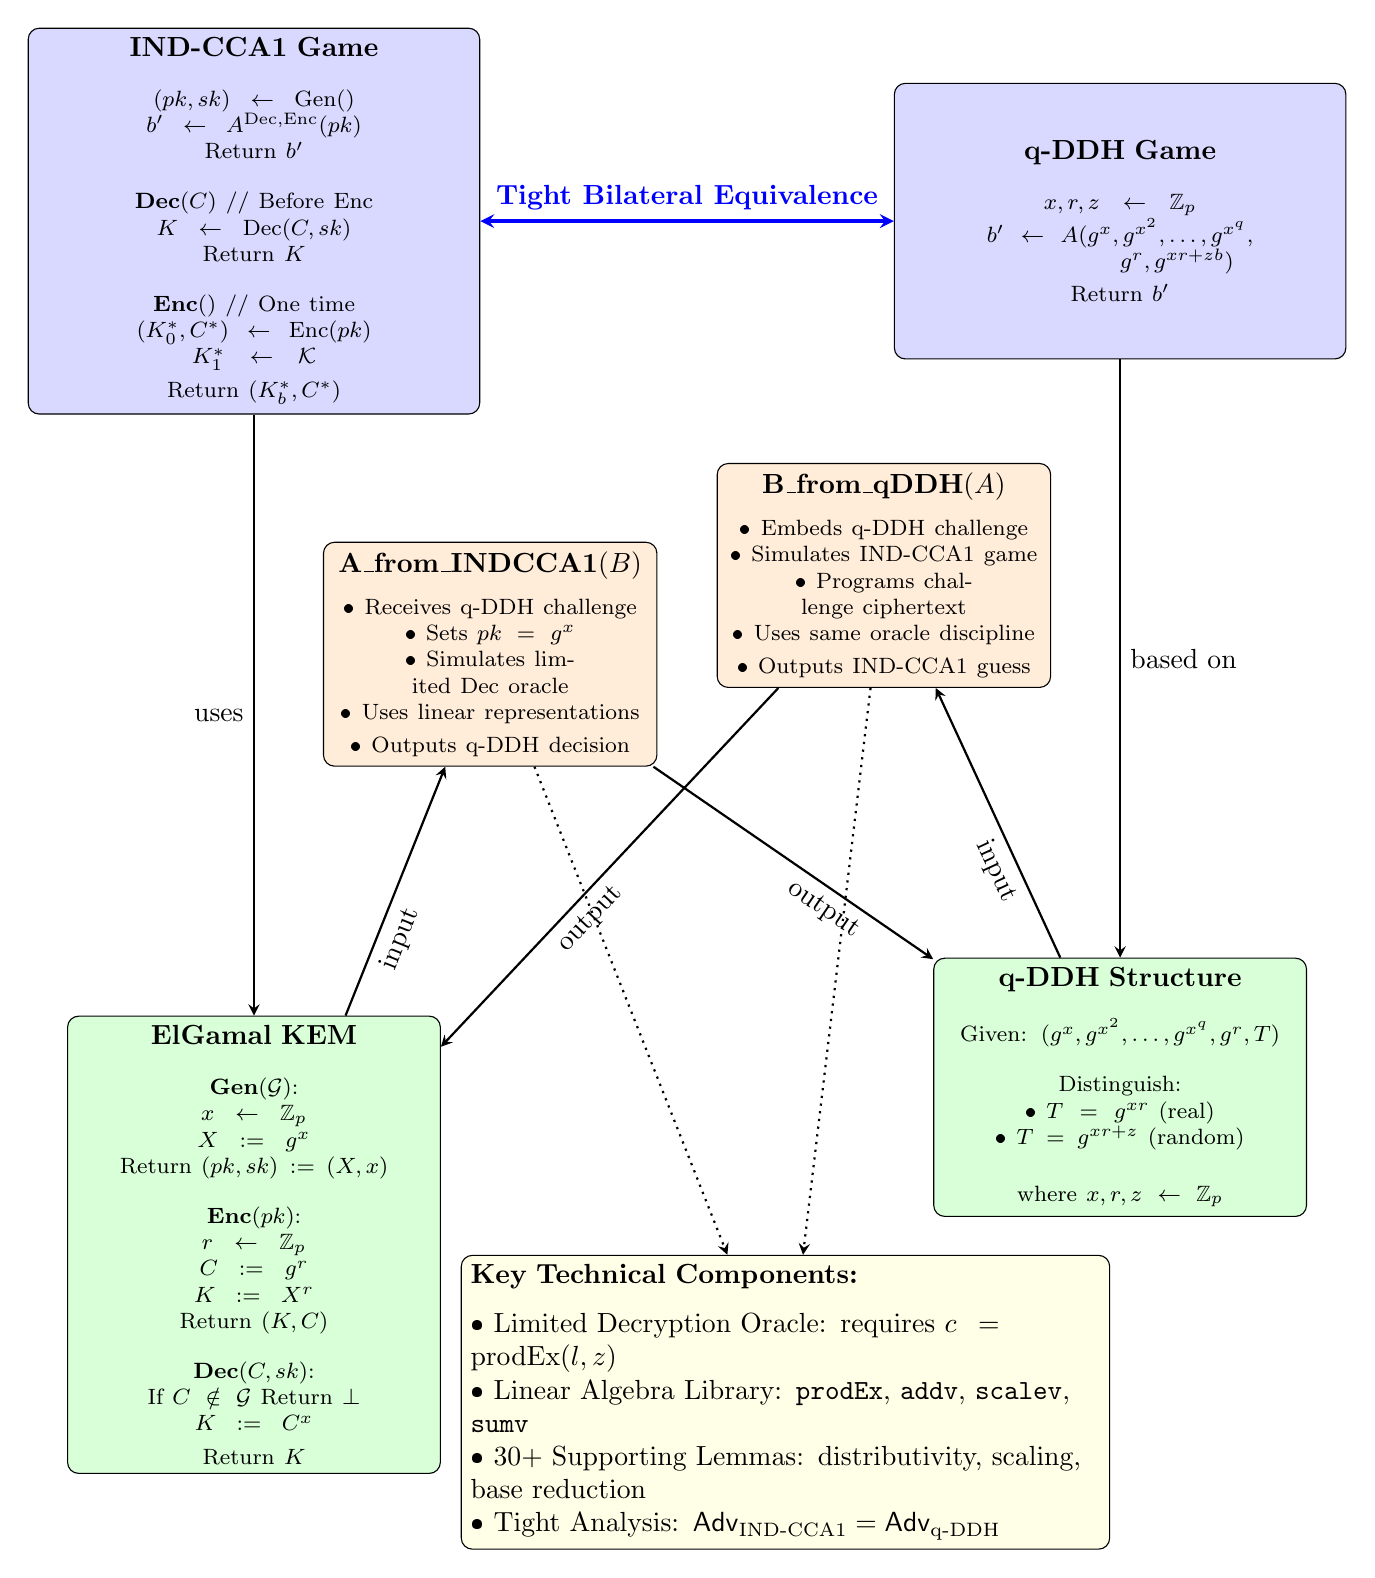
\begin{tikzpicture}[
    node distance=3cm,
    game/.style={rectangle, draw, fill=blue!15, text width=5.5cm, text centered, minimum height=3.5cm, rounded corners=4pt},
    scheme/.style={rectangle, draw, fill=green!15, text width=4.5cm, text centered, minimum height=2.8cm, rounded corners=4pt},
    reduction/.style={rectangle, draw, fill=orange!15, text width=4cm, text centered, minimum height=2cm, rounded corners=4pt},
    arrow/.style={->, thick, >=stealth},
    equiv/.style={<->, very thick, blue, >=stealth}
]

% IND-CCA1 Game
\node[game] (indcca-game) at (-10.5,5) {
    \textbf{IND-CCA1 Game}\\[0.3cm]
    \footnotesize
     $(pk, sk) \leftarrow \text{Gen}()$\\
     $b' \leftarrow A^{\text{Dec},\text{Enc}}(pk)$\\
     Return $b'$\\[0.3cm]
    \textbf{Dec}$(C)$ // Before Enc\\
     $K \leftarrow \text{Dec}(C, sk)$\\
     Return $K$\\[0.3cm]
    \textbf{Enc}$()$ // One time\\
     $(K_0^*, C^*) \leftarrow \text{Enc}(pk)$\\
     $K_1^* \leftarrow \mathcal{K}$\\
     Return $(K_b^*, C^*)$
};

% q-DDH Game  
\node[game] (qddh-game) at (0.5,5) {
    \textbf{q-DDH Game}\\[0.3cm]
    \footnotesize
     $x, r, z \leftarrow \mathbb{Z}_p$\\
     $b' \leftarrow A(g^x, g^{x^2}, \ldots, g^{x^q},$\\
    \phantom{01 $b' \leftarrow A($}$g^r, g^{xr+zb})$\\
     Return $b'$
};

% ElGamal Scheme
\node[scheme] (elgamal) at (-10.5,-8) {
    \textbf{ElGamal KEM}\\[0.3cm]
    \footnotesize
    \textbf{Gen}$(\mathcal{G})$:\\
     $x \leftarrow \mathbb{Z}_p$\\
     $X := g^x$\\
    Return $(pk, sk) := (X, x)$\\[0.3cm]
    \textbf{Enc}$(pk)$:\\
     $r \leftarrow \mathbb{Z}_p$\\
    $C := g^r$\\
     $K := X^r$\\
     Return $(K, C)$\\[0.3cm]
    \textbf{Dec}$(C, sk)$:\\
     If $C \notin \mathcal{G}$ Return $\perp$\\
     $K := C^x$\\
     Return $K$
};

% q-DDH Problem Structure
\node[scheme] (qddh-structure) at (0.5,-6) {
    \textbf{q-DDH Structure}\\[0.3cm]
    \footnotesize
    Given: $(g^x, g^{x^2}, \ldots, g^{x^q}, g^r, T)$\\[0.3cm]
    Distinguish:\\
    • $T = g^{xr}$ (real)\\
    • $T = g^{xr+z}$ (random)\\[0.3cm]
    where $x, r, z \leftarrow \mathbb{Z}_p$
};
% Forward Reduction
\node[reduction] (forward-red) at (-7.5,-0.5) {
    \textbf{${\text{A\_from\_INDCCA1}}(B)$}\\[0.2cm]
    \footnotesize
    • Receives q-DDH challenge\\
    • Sets $pk = g^x$\\
    • Simulates limited Dec oracle\\
    • Uses linear representations\\
    • Outputs q-DDH decision
};

% Backward Reduction
\node[reduction] (backward-red) at (-2.5,0.5) {
    \textbf{${\text{B\_from\_qDDH}}(A)$}\\[0.2cm]
    \footnotesize
    • Embeds q-DDH challenge\\
    • Simulates IND-CCA1 game\\
    • Programs challenge ciphertext\\
    • Uses same oracle discipline\\
    • Outputs IND-CCA1 guess
};
% Main equivalence
\draw[equiv] (indcca-game) -- (qddh-game) node[midway, above] {\textbf{Tight Bilateral Equivalence}};

% Connections to schemes
\draw[arrow] (indcca-game) -- (elgamal) node[midway, left] {uses};
\draw[arrow] (qddh-game) -- (qddh-structure) node[midway, right] {based on};

% Reduction arrows
\draw[arrow] (elgamal) -- (forward-red) node[midway, below left, sloped] {input};
\draw[arrow] (forward-red) -- (qddh-structure) node[midway, below right, sloped] {output};

\draw[arrow] (qddh-structure) -- (backward-red) node[midway, below right, sloped] {input};
\draw[arrow] (backward-red) -- (elgamal) node[midway, below left, sloped] {output};

% Oracle simulation details
\node[draw, fill=yellow!10, text width=8cm, rounded corners] (oracle-details) at (-3.75,-10) {
    \textbf{Key Technical Components:}\\[0.2cm]
    • Limited Decryption Oracle: requires $c = \text{prodEx}(l, z)$\\
    • Linear Algebra Library: \texttt{prodEx}, \texttt{addv}, \texttt{scalev}, \texttt{sumv}\\
    • 30+ Supporting Lemmas: distributivity, scaling, base reduction\\
    • Tight Analysis: $\mathsf{Adv}_{\text{IND-CCA1}} = \mathsf{Adv}_{\text{q-DDH}}$
};

\draw[arrow, dotted] (forward-red) -- (oracle-details);
\draw[arrow, dotted] (backward-red) -- (oracle-details);

\end{tikzpicture}
\caption{Detailed bilateral reduction between IND-CCA1 security of ElGamal-based \KEM and \qDDH hardness, showing the complete game structures and algorithmic details.}
\label{fig:detailed-bilateral-reduction}
\end{figure}




\section{Technical Overview}

Figure~\ref{fig:detailed-bilateral-reduction} indicates an intuitive overview of our proof technique.
At a high level, our goal is to show that the capability to break the IND-CCA1 security of the ElGamal-based \KEM\ is computationally equivalent to handling the \qDDH\ problem. 
Instead of relying on a one-way reduction, our analysis establishes a \emph{two-direction correspondence}—showing that both can be transformed into the other without any meaningful loss.

The proof process by building two designed reductions. 
In the \textbf{first direction}, we indicate that any adversary ability to breaking the ElGamal \KEM\ under chosen-ciphertext attacks can be covert into an algorithm that handle the \qDDH\ challenge. 
In the \textbf{reverse direction}, we demonstrate that a successful \qDDH\ distinguisher can be used to build an adversary that breaks the \KEM.

A key technical component is the leverage of \textbf{algebraic tracking}, where every group element generated during the simulation is represented as a linear combination of previously known ones. 
This idea, inspired by the Algebraic Group Model~\cite{cong2022}, ensures that simulated oracles behave consistently and ensures every adversarial action has a verifiable algebraic explanation.

Finally, the entire framework, containing oracle simulations, linear algebra operators (\texttt{prodEx}, \texttt{addv}, \texttt{scalev}, and \texttt{sumv}), and supporting lemmas—is implemented and mechanically verified in the \textsc{EasyCrypt} proof assistant, which guarantees the correspondence between the two games is not only theoretically sound but also \emph{machine-checked}.


% \subsection{Problem Structure and Games}

% The foundation of proof lies in the characterization of two computation problems:

% \subsubsection{IND-CCA1 Security Game.} 

% The indistinguishability under chosen-ciphertext attacks (IND-CCA1) security game for ElGamal \KEM proceeds as follows: The challenger first introduce a key pair $\text{Gen}()\rightarrow(pk,sk)$ where $pk = g^x$ and $sk = x$ for a randomly chosen $x \leftarrow \mathbb{Z}_p$. Then, the adversary $A$ is given the public key $pk$ and then make decryption queries to a oracle $\text{Dec}(C, sk)$ that returns $K = C^x$ for valid ciphertexts $C \in \mathcal{G}$. At some point, the adversary requests a challenge by calling the encryption oracle only once. The challenger computes $ \text{Enc}(pk)\rightarrow(K_0^*, C^*)$ where $C^* = g^r$ and $K_0^* = (g^x)^r = g^{xr}$ for a  random $ \mathbb{Z}_p \rightarrow r$, then selects a random key $ \mathcal{K} \rightarrow K_1^*$, and finally return $(K_b^*, C^*)$ for a random bit $b$. Finally, The adversary will outputs a guess $b'$ and wins if $b' = b$.

% The algorithm specification\cite{fuchsbauer2018} is detailed in Figure~\ref{fig:indcca1-algorithm}.

% \begin{figure}[H]
% \centering
% \footnotesize
% \begin{tabular}{|p{15cm}|}
% \hline
% \multicolumn{1}{|c|}{\textbf{IND-CCA1$_{\text{EG},\mathcal{G}}^A$ Security Game for ElGamal}} \\
% \hline
% \textbf{Algorithm:} \\
% 00 $x \leftarrow \mathbb{Z}_p$ \\
% 01 $X := g^x$ \\
% 02 $b' \leftarrow A^{\text{Dec},\text{Enc}}(X)$ \\
% 03 Return $b'$ \\
% \hline
% \textbf{Oracles Available to Adversary } $A$\textbf{:} \\
% $\bullet$ \textbf{Dec}$(C)_a$ // Before Enc is called \\
% \phantom{$\bullet$} 04 If $C \notin \mathcal{G}$ Return $\perp$ \\
% \phantom{$\bullet$} 05 $K := C^x$ \\
% \phantom{$\bullet$} 06 Return $K$ \\
% \\
% $\bullet$ \textbf{Enc}$()$ // One time only \\
% \phantom{$\bullet$} 07 $r \leftarrow \mathbb{Z}_p$ \\
% \phantom{$\bullet$} 08 $C^* := g^r$ \\
% \phantom{$\bullet$} 09 $K^* := X^r$ \\
% \phantom{$\bullet$} 10 $K_1^* \leftarrow \mathcal{K}$ // random key \\
% \phantom{$\bullet$} 11 $b \leftarrow \{0,1\}$ \\
% \phantom{$\bullet$} 12 Return $(K_b^*, C^*)$ \\
% \hline
% \textbf{ElGamal KEM Operations:} \\
% $\bullet$ \textbf{Gen}$(\mathcal{G}) \rightarrow (pk, sk)$: $x \leftarrow \mathbb{Z}_p$; $X := g^x$; Return $(X, x)$ \\
% $\bullet$ \textbf{Enc}$(pk) \rightarrow (K, C)$: $r \leftarrow \mathbb{Z}_p$; $C := g^r$; $K := pk^r$; Return $(K, C)$ \\
% $\bullet$ \textbf{Dec}$(C, sk) \rightarrow K$: If $C \notin \mathcal{G}$ Return $\perp$; $K := C^{sk}$; Return $K$ \\
% \hline
% \textbf{Advantage Definition:} \\
% $\mathsf{Adv}^{\text{IND-CCA1}}_{\text{ElGamal}}(A) = \left|\Pr[b' = b] - \frac{1}{2}\right|$ \\
% where $b$ is the random bit used in the Enc oracle \\
% \hline
% \textbf{Security Goal:} \\
% Adversary $A$ should not be able to distinguish between $K_0^* = g^{xr}$ (real key) and $K_1^*$ (random key) \\
% even with access to decryption oracle before receiving the challenge $(K_b^*, C^*)$ \\
% \hline
% \end{tabular}
% \caption{IND-CCA1 security game for ElGamal encryption. The adversary has access to a decryption oracle before the challenge phase, then must distinguish between a real session key and a random key.}
% \label{fig:indcca1-algorithm}
% \end{figure}






% \subsubsection{q-DDH Problem.} The q-Decisional Diffie-Hellman (q-DDH) problem will ask one to distinguish between two distributions over group elements. 
% By given a tuple $(g^x, g^{x^2}, \ldots, g^{x^q}, g^r, T)$ where $x, r \leftarrow \mathbb{Z}_p$ are random, the attacker must determine whether $T = g^{xr}$ (real distribution) or $T = g^{xr+z}$ for a random $z \leftarrow \mathbb{Z}_p$ (random distribution).

% The specification\cite{fuchsbauer2018} is detailed below in Figure~\ref{fig:qddh-algorithm}.


% \begin{figure}[H]
% \centering
% \footnotesize
% \begin{tabular}{|p{15cm}|}
% \hline
% \multicolumn{1}{|c|}{\textbf{q-DDH$_{\mathcal{G},q}^A$ Problem}} \\
% \hline
% \textbf{Algorithm:} \\
% 00 $x, r, z \leftarrow \mathbb{Z}_p$ \\
% 01 $b \leftarrow \{0,1\}$ \\
% 02 $T_0 := g^{xr}$, $T_1 := g^{xr+z}$ \\
% 03 $b' \leftarrow A(g^x, g^{x^2}, \ldots, g^{x^q}, g^r, T_b)$ \\
% 04 Return $b'$ \\
% \hline
% \textbf{Challenge Structure Given to Distinguisher } $A$\textbf{:} \\
% $\bullet$ \textbf{Powers of } $x$: $(g^x, g^{x^2}, g^{x^3}, \ldots, g^{x^q})$ \\
% $\bullet$ \textbf{Random element:} $g^r$ where $r \leftarrow \mathbb{Z}_p$ \\
% $\bullet$ \textbf{Target element:} $T \in \{g^{xr}, g^{xr+z}\}$ where $z \leftarrow \mathbb{Z}_p$ \\
% \hline
% \textbf{Distinguishing Goal:} \\
% $\bullet$ \textbf{Real distribution } $\mathcal{D}_0$: $T = g^{xr}$ (DDH tuple) \\
% $\bullet$ \textbf{Random distribution } $\mathcal{D}_1$: $T = g^{xr+z}$ (random element) \\
% \\
% Distinguisher $A$ must output a bit $b'$ indicating which distribution the challenge comes from \\
% \hline
% \textbf{Advantage Definition:} \\
% $\mathsf{Adv}^{q\text{-DDH}}_{\mathcal{G}}(A) = \left|\Pr[A(\mathcal{D}_0) = 1] - \Pr[A(\mathcal{D}_1) = 1]\right|$ \\
% where $\mathcal{D}_0 = (g^x, g^{x^2}, \ldots, g^{x^q}, g^r, g^{xr})$ \\
% and $\mathcal{D}_1 = (g^x, g^{x^2}, \ldots, g^{x^q}, g^r, g^{xr+z})$ \\
% \hline
% \textbf{Hardness Assumption:} \\
% For any probabilistic polynomial-time algorithm $A$: \\
% $\mathsf{Adv}^{q\text{-DDH}}_{\mathcal{G}}(A) \leq \text{negl}(\lambda)$ \\
% \\
% The q-DDH assumption states that even given the first $q$ powers of $x$, \\
% it remains computationally hard to distinguish $g^{xr}$ from $g^{xr+z}$ \\
% \hline
% \textbf{Relationship to Standard DDH:} \\
% $\bullet$ Standard DDH: Given $(g^a, g^b, g^c)$, distinguish $c = ab$ from random $c$ \\
% $\bullet$ q-DDH: Given $(g^x, \ldots, g^{x^q}, g^r, T)$, distinguish $T = g^{xr}$ from $T = g^{xr+z}$ \\
% $\bullet$ q-DDH $\Rightarrow$ DDH but the converse may not hold \\
% \hline
% \end{tabular}
% \caption{q-DDH (q-Decisional Diffie-Hellman) problem. The distinguisher receives the first $q$ powers of a secret exponent $x$ along with $g^r$ and must distinguish between $g^{xr}$ and $g^{xr+z}$ for random $z$.}
% \label{fig:qddh-algorithm}
% \end{figure}
















% \subsection{Bilateral Reduction Strategy}

% Our core technical contribution is the establishment of two reductions that bridge computational equivalence between:

% \subsubsection{Forward Reduction: ${\text{A\_from\_INDCCA1}}$.} This reduction will convert all IND-CCA1 adversary $B$ against ElGamal into a q-DDH distinguisher.,which works as follows:
% \begin{enumerate}
% \item \textbf{Challenge Reception:} It will first receiving a q-DDH challenge $(g^x, g^{x^2}, \ldots, g^{x^q}, g^r, T)$, then set the public key as $pk = g^x$.
% \item \textbf{Oracle Simulation:} Then it will leverage a limited decryption oracle that only processes queries $(C, z)$ where  adversary provides an explicit linear representation $z$ such that $C = \text{prodEx}(l, z)$, while $l = [g, g^x, \text{previous\_results}]$ is the list of group elements already known.
% \item \textbf{Challenge Programming:} Finally the adversary is expected to request the encryption challenge, that sets $C^* = g^r$ and $K^* = T$, giving the q-DDH challenge directly into the IND-CCA1 game.
% \item \textbf{Decision Extraction:} The reduction outputs the adversary's guess as its q-DDH decision.
% \end{enumerate}

% \subsubsection{Backward Reduction: ${\text{B\_from\_qDDH}}$.} This reduction converts any q-DDH distinguisher $A$ into an IND-CCA1 adversary:
% \begin{enumerate}
% \item \textbf{Challenge Embedding:} The reduction embeds the received IND-CCA1 challenge into a q-DDH problem by generating the tuple $(g^x, g^{x^2}, \ldots, g^{x^q}, C^*, K^*)$ where $x$ is the secret key and $(K^*, C^*)$ is the challenge key-ciphertext pair.
% \item \textbf{Game Simulation:} Then it will simulates the q-DDH game for the attacker by the same oracle discipline as the forward reduction.
% \item \textbf{Advantage Preservation:} The distinguisher's decision is directly translated into an IND-CCA1 guess.
% \end{enumerate}









\subsection{Key Technical Components}

The success of our formalized proof of bilateral reduction relies on several sophisticated technical innovations:

\subsubsection{Limited Decryption Oracle.} The basic of our approach is a constrained decryption oracle that requires adversaries to provide algebraic representations for their queries. Specifically, for any decryption query $(C, z)$, the oracle will verify that $C = \text{prodEx}(l, z)$ where $l$ is the current list of known group elements and $z$ is a vector of exponents. This restriction ensures:
\begin{itemize}
\item The simulator will not be request to expose information of discrete logarithms
\item All group elements have explicit linear representations by the generation of adversary 
\item The oracle simulation maintain consistency in both directions . 
\end{itemize}

\subsubsection{Linear Algebra Library.} We develop a comprehensive library of operators and lemmas for manipulating linear combinations in the exponent field:
\begin{itemize}
\item \textbf{Core Operators:} \texttt{prodEx} (product of exponentiations), \texttt{addv} (vector addition), \texttt{scalev} (scalar multiplication), \texttt{sumv} (vector summation), and \texttt{shift\_trunc} (shift and truncate for alignment)
\item \textbf{Algebraic Properties:} Over 30 supporting lemmas covering distributivity, scaling laws, base reduction, zero-vector properties, and shift-truncate compatibility
\item \textbf{Consistency Guarantees:} All operations preserve the correspondence between linear algebra in the exponent field and group operations
\end{itemize}

\subsubsection{Representation Tracking.} Throughout both direction of reductions, we maintain discipline of tracking the linear representations of all group elements that enables:
\begin{itemize}
\item Consistent oracle simulation without exposure of knowledge of secret keys
\item Tight security analysis with no loss in adversarial advantages
\item Modular proof structure that can be extended 
\end{itemize}
















\subsection{Formal Verification Infrastructure}

Our entire proof is fully mechanized in the EasyCrypt , cosists of over 2000 lines of verified code. The formalization provides not only a transformation of the paper proof ~\cite{fuchsbauer2018} into mechanized, but also offering a methodological contribution in its own right. Specifically, it provides benefits specified below that strengthen both the soundness and reusability:



\begin{itemize}
\item \textbf{Complete Mechanization:} Every aspect of the security argument, such as game transformations, oracle simulations and algebraic manipulations has been expressed by EasyCrypt. Unlike paper proofs, there is no step left at the intuitive level, in particular, the boundary condition and random variable transformation is completely strictly formalized.





\item \textbf{Modular Design:} 
The development makes contribution of  a dedicated linear-algebra library with a reusable reduction components. These modules are  designed to be generic and independent of ElGamal itself, enable them to be applied to a broader range of AGM-style proof, for instance, make proofs for digital signatures, polynomial commitments and so on.


\item \textbf{Reproducible Results:}  Due to the proof is fully mechanized, it can be independently rerun, checked, and extended by future researchers, that ensures the results are not only correct once,  but keep verifiable as the EasyCrypt platform evolves. Future researchers can build on this code-base as a foundation for more complex cryptographic proofs on AGM.








\item \textbf{Hidden Assumption Elimination:} Formal verification requires the proof to expose all implicit requirements. Subtleties that might be informally justified in paper proof, for instance, vector length constraints and randomness-preserving bijections are  discharged mechanically by EasyCrypt, which prevents the presence of unstated assumptions and ensures the security reduction is strictly formalized and accurate.




\end{itemize}

All in all, this aspects above indicates that the IND-CCA1 security of ElGamal and the hardness of the q-DDH problem are not only related through a reduction, but are computationally equivalent with perfect tightness. Additionally, our contribution is more than just a reimplementation of a known proof but a carefully formalized, reproducible and reusable approach.

                  % introduction
\chapter{Background}\label{chap:background}



This section introduces the EasyCrypt verification framework and provides essential background on the algebraic group model that forms our analysis.

\section{The EasyCrypt Verification Framework}
\label{sec:easycrypt-framework}

EasyCrypt~\cite{easycrypt} serves as our basic framework for mechanizing cryptographic security arguments. This tool specializes in formalizing and verifying security proofs for cryptographic constructions through rigorous mathematical reasoning. The coreof EasyCrypt is its Probabilistic Relational Hoare Logic (pRHL), which we utilize extensively throughout our bilateral equivalence proof to build exact correspondences between security games while maintaining control over probabilistic reasoning~\cite{Bar2012}.

Probabilistic Relational Hoare Logic (pRHL) enables us to establish that corresponding executions across different game contexts maintain identical success probabilities without requiring detailed characterization of intermediate distributions. Such relational reasoning proves particularly powerful for our tight reduction, where the primary objective is demonstrating perfect correspondence between adversarial advantages rather than computing absolute probability values~\cite{kyber2024}.

While EasyCrypt's standard reasoning strategies handle the majority of our proof obligations, certain technical steps in our bilateral reduction demand more sophisticated approaches that require global program analysis and explicit management of algebraic relationships. These include randomness-preserving transformations and complex oracle simulations that must maintain consistency across multiple game contexts. EasyCrypt addresses these requirements through specialized reasoning techniques and transformation rules, though their direct application requires careful orchestration in our specific proof context.

To address this complexity, the EasyCrypt ecosystem has evolved to include a comprehensive collection of generic libraries that encapsulate common cryptographic proof patterns into reusable components. These libraries abstract intricate reasoning steps into high-level "game transformation" lemmas and equivalence theorems that can be instantiated and composed within larger security arguments.


The formal verification process encompasses over 2000 lines of verified EasyCrypt code, representing one of the most substantial mechanizations of AGM-style reasoning to date. This level of formalization provides unprecedented confidence in the correctness of our security argument while establishing reusable infrastructure for future research in mechanized cryptographic verification.


\subsection{Core Concepts}

EasyCrypt operates on several key principles that make it particularly suitable for cryptographic analysis:

\paragraph{Probabilistic Relational Hoare Logic (pRHL).} EasyCrypt's cornerstone is probabilistic Relational Hoare Logic (pRHL), which enables reasoning about relationships between probabilistic programs~\cite{Bar2012}. In our context, pRHL allows us to establish probability equalities between different cryptographic games, such as our main lemma:
\[
\Pr[\text{IND\_CCA1\_P}(\text{ElGamal}, B).\text{main}() : \text{res}] = \Pr[\text{QDDH}(A_{\text{from\_INDCCA1}}(B)).\text{main}() : \text{res}]
\]

\paragraph{Game Transformations.} EasyCrypt provides several powerful tactics for transforming games while preserving their probability distributions:

\begin{itemize}
\item \textbf{byequiv transformations}: These are built upon pRHL and allow us to prove that two games have identical probability distributions by establishing a relational invariant between their executions.

\item \textbf{bypr transformations}: These enable reasoning about probability bounds and are particularly useful for establishing security reductions.

\item \textbf{rnd transformations}: These are pRHL-based tactics for reasoning about randomness. For example, in our proof we use:
\begin{lstlisting}[style=easycrypt, basicstyle=\footnotesize\ttfamily]
rnd (fun k' => loge k' - sk0{1} * y{1}) 
    (fun z => g ^ (z + sk0{1} * y{1})).
\end{lstlisting}
This transformation converts randomness from group elements to the exponent field, making the two games probabilistically equivalent.
\end{itemize}

\paragraph{Oracle Simulation.} EasyCrypt excels at reasoning about oracle-based security games. In our work, pRHL is crucial for:
\begin{itemize}
\item \textbf{Correctness}: Ensuring that simulated oracles produce the same outputs as real oracles for valid queries
\item \textbf{State Management}: Tracking the evolution of oracle state across game executions  
\item \textbf{Query Validation}: Verifying that adversarial queries satisfy the required algebraic constraints
\end{itemize}



\section{Background: Algebraic Group Model}
\label{sec:agm-background}

The Algebraic Group Model (AGM), introduced by Fuchsbauer, Kiltz, and Loss~\cite{fuchsbauer2018}, provides a framework for analyzing cryptographic schemes by restricting adversaries to be "algebraic."

In particular, instead of assuming an all-powerful attacker, the AGM will restricts adversaries to be algebraic, meaning that whenever they generate a new group element, they must also explain how it was algebraically derived from elements they have already seen~\cite{cong2022}. This model indicates the intuition that real cryptographic algorithms operate through concrete algebraic operations, rather than arbitrary black-box calculations.
By constrain adversaries in certain way, the AGM provides a intermediate position between the idealized models, such as the Random Oracle Model, and the entirely general Standard Model, allowing proofs to achieve a balance between realistic and easy to formalize.

\begin{definition}[Algebraic Adversary]
\label{def:algebraic-adversary}
An adversary $\mathcal{A}$ is algebraic if, whenever it outputs a group element $h \in \mathcal{G}$, it also provides a representation vector $\mathbf{z} = (z_1, \ldots, z_k) \in \mathbb{Z}_p^k$ such that:
\[
h = \prod_{i=1}^k g_i^{z_i}
\]
where $g_1, \ldots, g_k$ are all group elements that $\mathcal{A}$ has seen so far.
\end{definition}

The AGM assumption enables tighter security reductions by providing the reduction algorithm with algebraic representations of adversarial outputs, effectively giving the reduction "extraction" capabilities without explicit knowledge extraction.

\begin{assumption}[AGM Assumption]
\label{ass:agm}
All adversaries are algebraic in the sense of Definition~\ref{def:algebraic-adversary}.
\end{assumption}

This assumption is particularly well-suited for analyzing discrete logarithm-based schemes like ElGamal, as it captures the natural algebraic structure that such schemes possess while remaining weaker than the generic group model.


\section{Games framework}

The foundation of our proof lies in the characterization of two computation problems:

\subsection{IND-CCA1 Security Game for ElGamal.} 

The indistinguishability under chosen-ciphertext attacks (IND-CCA1) security game for ElGamal \KEM proceeds as follows: The challenger first introduce a key pair $\text{Gen}()\rightarrow(pk,sk)$ where $pk = g^x$ and $sk = x$ for a randomly chosen $x \leftarrow \mathbb{Z}_p$. Then, the adversary $A$ is given the public key $pk$ and then make decryption queries to a oracle $\text{Dec}(C, sk)$ that returns $K = C^x$ for valid ciphertexts $C \in \mathcal{G}$. At some point, the adversary requests a challenge by calling the encryption oracle only once. The challenger computes $ \text{Enc}(pk)\rightarrow(K_0^*, C^*)$ where $C^* = g^r$ and $K_0^* = (g^x)^r = g^{xr}$ for a  random $ \mathbb{Z}_p \rightarrow r$, then selects a random key $ \mathcal{K} \rightarrow K_1^*$, and finally return $(K_b^*, C^*)$ for a random bit $b$. Finally, The adversary will outputs a guess $b'$ and wins if $b' = b$.

The algorithm specification\cite{fuchsbauer2018} is detailed in Figure~\ref{fig:indcca1-algorithm}.

\begin{figure}[H]
\centering
\footnotesize
\begin{tabular}{|p{15cm}|}
\hline
\multicolumn{1}{|c|}{\textbf{IND-CCA1$_{\text{EG},\mathcal{G}}^A$ Security Game for ElGamal}} \\
\hline
\textbf{Algorithm:} \\
00 $x \leftarrow \mathbb{Z}_p$ \\
01 $X := g^x$ \\
02 $b' \leftarrow A^{\text{Dec},\text{Enc}}(X)$ \\
03 Return $b'$ \\
\hline
\textbf{Oracles Available to Adversary } $A$\textbf{:} \\
$\bullet$ \textbf{Dec}$(C)_a$ // Before Enc is called \\
\phantom{$\bullet$} 04 If $C \notin \mathcal{G}$ Return $\perp$ \\
\phantom{$\bullet$} 05 $K := C^x$ \\
\phantom{$\bullet$} 06 Return $K$ \\
\\
$\bullet$ \textbf{Enc}$()$ // One time only \\
\phantom{$\bullet$} 07 $r \leftarrow \mathbb{Z}_p$ \\
\phantom{$\bullet$} 08 $C^* := g^r$ \\
\phantom{$\bullet$} 09 $K^* := X^r$ \\
\phantom{$\bullet$} 10 $K_1^* \leftarrow \mathcal{K}$ // random key \\
\phantom{$\bullet$} 11 $b \leftarrow \{0,1\}$ \\
\phantom{$\bullet$} 12 Return $(K_b^*, C^*)$ \\
\hline
\textbf{ElGamal KEM Operations:} \\
$\bullet$ \textbf{Gen}$(\mathcal{G}) \rightarrow (pk, sk)$: $x \leftarrow \mathbb{Z}_p$; $X := g^x$; Return $(X, x)$ \\
$\bullet$ \textbf{Enc}$(pk) \rightarrow (K, C)$: $r \leftarrow \mathbb{Z}_p$; $C := g^r$; $K := pk^r$; Return $(K, C)$ \\
$\bullet$ \textbf{Dec}$(C, sk) \rightarrow K$: If $C \notin \mathcal{G}$ Return $\perp$; $K := C^{sk}$; Return $K$ \\
\hline
\textbf{Advantage Definition:} \\
$\mathsf{Adv}^{\text{IND-CCA1}}_{\text{ElGamal}}(A) = \left|\Pr[b' = b] - \frac{1}{2}\right|$ \\
where $b$ is the random bit used in the Enc oracle \\
\hline
\textbf{Security Goal:} \\
Adversary $A$ should not be able to distinguish between $K_0^* = g^{xr}$ (real key) and $K_1^*$ (random key) \\
even with access to decryption oracle before receiving the challenge $(K_b^*, C^*)$ \\
\hline
\end{tabular}
\caption{IND-CCA1 security game for ElGamal encryption. The adversary has access to a decryption oracle before the challenge phase, then must distinguish between a real session key and a random key.}
\label{fig:indcca1-algorithm}
\end{figure}






\subsection{q-DDH Problem.} The q-Decisional Diffie-Hellman (q-DDH) problem will ask one to distinguish between two distributions over group elements. 
By given a tuple $(g^x, g^{x^2}, \ldots, g^{x^q}, g^r, T)$ where $x, r \leftarrow \mathbb{Z}_p$ are random, the attacker must determine whether $T = g^{xr}$ (real distribution) or $T = g^{xr+z}$ for a random $z \leftarrow \mathbb{Z}_p$ (random distribution).

The specification\cite{fuchsbauer2018} is detailed below in Figure~\ref{fig:qddh-algorithm}.


\begin{figure}[H]
\centering
\footnotesize
\begin{tabular}{|p{15cm}|}
\hline
\multicolumn{1}{|c|}{\textbf{q-DDH$_{\mathcal{G},q}^A$ Problem}} \\
\hline
\textbf{Algorithm:} \\
00 $x, r, z \leftarrow \mathbb{Z}_p$ \\
01 $b \leftarrow \{0,1\}$ \\
02 $T_0 := g^{xr}$, $T_1 := g^{xr+z}$ \\
03 $b' \leftarrow A(g^x, g^{x^2}, \ldots, g^{x^q}, g^r, T_b)$ \\
04 Return $b'$ \\
\hline
\textbf{Challenge Structure Given to Distinguisher } $A$\textbf{:} \\
$\bullet$ \textbf{Powers of } $x$: $(g^x, g^{x^2}, g^{x^3}, \ldots, g^{x^q})$ \\
$\bullet$ \textbf{Random element:} $g^r$ where $r \leftarrow \mathbb{Z}_p$ \\
$\bullet$ \textbf{Target element:} $T \in \{g^{xr}, g^{xr+z}\}$ where $z \leftarrow \mathbb{Z}_p$ \\
\hline
\textbf{Distinguishing Goal:} \\
$\bullet$ \textbf{Real distribution } $\mathcal{D}_0$: $T = g^{xr}$ (DDH tuple) \\
$\bullet$ \textbf{Random distribution } $\mathcal{D}_1$: $T = g^{xr+z}$ (random element) \\
\\
Distinguisher $A$ must output a bit $b'$ indicating which distribution the challenge comes from \\
\hline
\textbf{Advantage Definition:} \\
$\mathsf{Adv}^{q\text{-DDH}}_{\mathcal{G}}(A) = \left|\Pr[A(\mathcal{D}_0) = 1] - \Pr[A(\mathcal{D}_1) = 1]\right|$ \\
where $\mathcal{D}_0 = (g^x, g^{x^2}, \ldots, g^{x^q}, g^r, g^{xr})$ \\
and $\mathcal{D}_1 = (g^x, g^{x^2}, \ldots, g^{x^q}, g^r, g^{xr+z})$ \\
\hline
\textbf{Hardness Assumption:} \\
For any probabilistic polynomial-time algorithm $A$: \\
$\mathsf{Adv}^{q\text{-DDH}}_{\mathcal{G}}(A) \leq \text{negl}(\lambda)$ \\
\\
The q-DDH assumption states that even given the first $q$ powers of $x$, \\
it remains computationally hard to distinguish $g^{xr}$ from $g^{xr+z}$ \\
\hline
\textbf{Relationship to Standard DDH:} \\
$\bullet$ Standard DDH: Given $(g^a, g^b, g^c)$, distinguish $c = ab$ from random $c$ \\
$\bullet$ q-DDH: Given $(g^x, \ldots, g^{x^q}, g^r, T)$, distinguish $T = g^{xr}$ from $T = g^{xr+z}$ \\
$\bullet$ q-DDH $\Rightarrow$ DDH but the converse may not hold \\
\hline
\end{tabular}
\caption{q-DDH (q-Decisional Diffie-Hellman) problem. The distinguisher receives the first $q$ powers of a secret exponent $x$ along with $g^r$ and must distinguish between $g^{xr}$ and $g^{xr+z}$ for random $z$.}
\label{fig:qddh-algorithm}
\end{figure}





                    % background/framework
\chapter{Related Work}\label{chap:relatedWork}

IND-CCA (Indistinguishability under Chosen Ciphertext Attack) security is a core concept in public-key cryptography. It requires that even when attackers can query a decryption oracle, they still cannot distinguish the target plaintext, thus providing one of the strongest confidentiality guarantees for encryption schemes. IND-CCA security proofs are often complex and tedious, and traditional manual reduction processes are prone to errors. To reduce this risk, the academic community has increasingly focused on formal verification tools such as EasyCrypt in recent years~\cite{easycrypt}. Barthe et al. first conducted mechanized verification of some conclusions that were previously only argued intuitively in the Generic Group Model (GGM). Furthermore, EasyCrypt has been used for formal verification of modern encryption schemes, such as the IND-CCA security of Kyber during the NIST standardization process, whose proof was completed through machine verification using the Fujisaki-Okamoto transformation under the random oracle model~\cite{kyber2024}.

Nevertheless, EasyCrypt also has limitations. Particularly, the library and ecosystem are still relatively underdeveloped, resulted in many commonly required basic lemmas and operators are not able to used directly, meaning that users are often required to implement basic algebraic machinery themselves in order to complete non-trivial proofs. This lack of readily reusable components increases the effort, but it also motivates the systematic development of reusable operators and lemmas, enriching EasyCrypt's ecosystem for future proof.

In this context, researchers have proposed some alternative models to obtain tighter or more concise security proofs. The most representative is the Algebraic Group Model (AGM) proposed by Fuchsbauer, Kiltz, and Loss~\cite{fuchsbauer2018}. In AGM, it is assumed that adversaries are algebraic, meaning that whenever they output a new group element, they must simultaneously provide a representation of how this element is formed by combining previous elements. This restriction provides additional structural information for reductions, making the proof process more concise and tight. A key result by the authors (Theorem 5.2) shows that breaking the IND-CCA1 security of ElGamal is tightly equivalent to solving the q-type DDH problem under AGM. This proof uses the algebraic representations provided by adversaries to construct consistent decryption oracle simulation, achieving an almost lossless security reduction.

The advantage of the AGM approach is that it provides tight reductions (no loss in attack advantage) and allows reasoning to avoid the complex guessing and technical rewinding common in standard model proofs. However, its limitations are also obvious: AGM relies on non-standard assumptions about adversaries, and existing proofs are still manual derivations that have not undergone mechanized verification. Although these proofs are highly convincing, some steps are still based on intuition rather than formal derivation, so potential subtle errors may still exist, which is precisely where formal methods can provide compensation.

Beyond encryption schemes, AGM has also been applied to more complex cryptographic protocols. In their 2023 work "From Polynomial IOP and Commitments to Non-malleable zkSNARKs," Faonio et al.~\cite{faonio2023} used AGM (combined with the random oracle model) to prove the simulation-extractability of the KZG polynomial commitment scheme, thereby constructing non-malleable zkSNARKs. This shows that AGM is also valuable in security analysis of complex protocols, especially in scenarios where direct proofs are difficult to provide in the standard model. However, similar to the ElGamal case, this work still remains at the manual proof level and has not achieved mechanized verification. This also indicates that there is still a gap between AGM-style reasoning and fully formal verification. How to combine intuitive algebraic reasoning with machine-verifiable formal methods remains an important challenge facing this field.

When it comes to the the ElGamal-based Key Encapsulation Mechanism (\KEM), which has been widely studied under various computational assumptions and application settings. Galindo et al.~\cite{galindo2016} introduced a leakage-resilient variant of the ElGamal KEM, named BEG-KEM, which enhances resistance against side-channel attacks through masking and blinding techniques while maintaining practical performance on embedded platforms. Hashimoto et al.~\cite{hashimoto2022} further strengthened the theoretical foundations by providing a tight reduction proof for the Twin-DH hashed ElGamal KEM in multi-user environments, demonstrating its scalability and security. Earlier, Kiltz and Pietrzak~\cite{kiltz2010} established one of the first leakage-resilient ElGamal constructions, proving that a CCA1-secure KEM combined with a one-time symmetric cipher can yield full \INDCCAone security even under bounded key leakage. Finally, Lee et al.~\cite{lee2023} introduced a decomposable KEM framework that achieves continuous key agreement with reduced bandwidth while retaining DDH-based security guarantees. 
Together, these works demonstrate the evolution of ElGamal-based KEMs from theoretical constructs toward efficient, leakage-resilient, and tightly secure primitives across a variety of cryptographic contexts.
                   % related work
\chapter{q-DDH Correctness and IND-CCA1 Security}
\label{sec:qddh-indcca1-security}

This part establishes the mathematical and cryptographic foundations required for our analysis. We first introduce the ElGamal Key Encapsulation Mechanism (KEM), providing its algorithmic description and a formalized implementation in EasyCrypt; subsequently, we define the IND-CCA1 security model; and finally introduce the q-Decisional Diffie–Hellman (q-DDH) assumption. These components provide a structured foundation for subsequent reasoning about accuracy and security, enabling reductions to be rigorously expressed within our EasyCrypt code.

\section{ElGamal Key Encapsulation Mechanism}
\label{sec:elgamal-kem}
Our analysis focuses on the KEM formulation of ElGamal, specifying three algorithms that operate over a cyclic group $\mathcal{G}$ of prime order $p$ with generator $g$. This formal description facilitates distinguishing correctness from security: correctness ensures legitimate recipients accurately recover encrypted session keys, while security ensures attackers cannot distinguish keys from random ones.

\subsection{Algorithmic Specification}

The ElGamal KEM is defined by the following algorithms:

\paragraph{Key Generation.}
\begin{algorithmic}[1]
\STATE \textbf{Algorithm} $\mathsf{KeyGen}(\mathcal{G}) \rightarrow (pk, sk)$:
\STATE $x \leftarrow \mathbb{Z}_p$ \COMMENT{Sample random secret key}
\STATE $pk \leftarrow g^x$ \COMMENT{Compute public key}
\STATE \textbf{return} $(pk, sk) = (g^x, x)$
\end{algorithmic}

\paragraph{Key Encapsulation.}
\begin{algorithmic}[1]
\STATE \textbf{Algorithm} $\mathsf{Enc}(pk) \rightarrow (K, C)$:
\STATE $r \leftarrow \mathbb{Z}_p$ \COMMENT{Sample random encapsulation exponent}
\STATE $C \leftarrow g^r$ \COMMENT{Compute ciphertext}
\STATE $K \leftarrow pk^r$ \COMMENT{Compute session key}
\STATE \textbf{return} $(K, C) = (g^{xr}, g^r)$
\end{algorithmic}

\paragraph{Key Decapsulation.}
\begin{algorithmic}[1]
\STATE \textbf{Algorithm} $\mathsf{Dec}(C, sk) \rightarrow K$:
\STATE \textbf{if} $C \notin \mathcal{G}$ \textbf{then return} $\perp$
\STATE $K \leftarrow C^{sk}$ \COMMENT{Recover session key}
\STATE \textbf{return} $K$
\end{algorithmic}

\subsection{EasyCrypt Implementation}

The ElGamal KEM is implemented in EasyCrypt as follows:

\begin{lstlisting}[style=easycrypt, caption=ElGamal KEM Implementation in EasyCrypt, breaklines=true, breakatwhitespace=true, frame=single, keepspaces=true]
(** ElGamal encryption scheme implementation **)
module ElGamal : Scheme = {
  (* Key generation: sk random, pk = g^sk *)
  proc keygen(): pk_t * sk_t = {
    var sk;
    sk <$ FD.dt;              (* Random secret key *)
    return (g ^ sk, sk);      (* Public key is g^sk *)
  }

  (* Encryption: return (pk^y, g^y) where y is random *)
  proc enc(pk:pk_t): key_t * ctxt_t= {
    var y;
    y <$ FD.dt;               (* Random encryption exponent *)
    return (pk ^ y, g ^ y);   (* Session key and ciphertext *)
  }
  
  (* Decryption: compute c^sk *)
  proc dec(c:ctxt_t,sk:sk_t): key_t option = {
    return Some (c ^ sk);     (* ElGamal decryption formula *)
  }
}.
\end{lstlisting}

\section{IND-CCA1 Security Model}
\label{sec:ind-cca1-model}

Indistinguishability under non-adaptive chosen-ciphertext attacks (IND-CCA1) is a significant security notion for public-key encryption schemes.

\begin{definition}[IND-CCA1 Security Game]
\label{def:ind-cca1-game}
For a KEM scheme $\mathsf{KEM} = (\mathsf{KeyGen}, \mathsf{Enc}, \mathsf{Dec})$ and adversary $\mathcal{A}$, the IND-CCA1 security game proceeds as follows:

\begin{algorithmic}[1]
\STATE $(pk, sk) \leftarrow \mathsf{KeyGen}()$ \COMMENT{Generate key pair}
\STATE $\mathcal{A}$ receives $pk$ and can query decryption oracle $\mathsf{Dec}(sk, \cdot)$
\STATE $(K_0, C^*) \leftarrow \mathsf{Enc}(pk)$ \COMMENT{Generate challenge}
\STATE $K_1 \leftarrow \mathcal{K}$ \COMMENT{Sample random key}
\STATE $b \leftarrow \{0,1\}$ \COMMENT{Choose challenge bit}
\STATE $b' \leftarrow \mathcal{A}(K_b, C^*)$ \COMMENT{Adversary distinguishes}
\STATE \textbf{return} $(b' = b)$ \COMMENT{Adversary wins if correct}
\end{algorithmic}
\end{definition}

The adversary's advantage is defined as:
\[
\mathsf{Adv}^{\text{IND-CCA1}}_{\mathsf{KEM}}(\mathcal{A}) = \left| \Pr[\text{IND-CCA1}^{\mathcal{A}}_{\mathsf{KEM}} = 1] - \frac{1}{2} \right|
\]

In the algebraic group model, the decryption oracle requires adversaries to provide algebraic representations for their queries, ensuring that all ciphertexts can be expressed in terms of previously seen group elements.

\subsection{Relationship to Other Security Notions}

Conceptually, IND-CCA1 strengthens IND-CPA by granting a decryption oracle only \emph{before} the challenge, while weaker than full adaptive IND-CCA2~\cite{fuchsbauer2018}.

In modern use, IND-CCA1 still occurs in settings where post-challenge oracle access is implausible (e.g., certain KEM/DEM designs under one-shot decryption exposure) or as a intermediate step to IND-CCA2. Formal treatments and exercises with complete games, oraclesand reductions can be found in standard texts and course notes~\cite{katzlindell-2nd,princeton-cramershoup}.

\subsection{Algebraic Oracle Implementation}

The key contribution in our formalization is the algebraic oracle that enforces AGM constraints through a two-layer design: interface abstraction and implementation with validation.

\paragraph{Interface Layer: Decryption Oracle Abstraction under AGM.}

We encode the phase-based constraints of the IND-CCA1 game directly into the type and effect system. The decryption oracle interface \texttt{Oracles\_CCA1i} provides initialization \texttt{init} and representation-based decryption \texttt{dec(c, z)}, where vector $z$ represents the algebraic representation of ciphertext group element $c$ relative to the visible base list $l$. The adversary interface \texttt{Adv\_INDCCA1} is decomposed into a ``scouting'' phase \texttt{scout(pk)} (allowing calls to \texttt{O.dec}) and a ``distinguishing'' phase \texttt{distinguish(k, c)} (prohibiting calls to \texttt{O.dec}).

This layered abstraction provides two benefits: First, the game rules (decryption allowed before challenge, forbidden after challenge) are enforced through effect annotations at the type level, avoiding the need to manually exclude illegal calls. Second, requiring representation $z$ makes explicit the core assumption of the Algebraic Group Model (AGM)---that adversaries must provide linear/exponential combinations relative to the ``known set'' $l$ for every queried group element, therefore strictly limiting the adversary's accessible information to the linear space generated by $l$ and enabling precise algebraic reasoning in subsequent reductions.

\begin{lstlisting}[style=easycrypt, caption=Algebraic Oracle Interface, breaklines=true, breakatwhitespace=true, frame=single, keepspaces=true]
(** Interface for oracles used in CCA1 security games **)
module type Oracles_CCA1i = {
  proc init(sk_init : sk_t) : unit                    (* Initialize with secret key *)
  proc dec(c : ctxt_t, z : exp list) : key_t option   (* Decryption with representation *)
}.

(** Adversary interface for IND-CCA1 game **)
module type Adv_INDCCA1 (O : Oracles_CCA1i) = {
  proc scout(pk : pk_t) : unit {O.dec}         (* Phase 1: explore with queries *)
  proc distinguish(k : key_t, c : ctxt_t) : bool {}  (* Phase 2: distinguish challenge *)
}.
\end{lstlisting}

\paragraph{Implementation Layer: Limited Oracle with Query Quota and Representation Validation.}

The module \texttt{O\_CCA1\_Limited} enforces both query quota and representation consistency validation at the implementation level. In \texttt{dec(c, z)} calls, a query is considered valid only when the quota is not exceeded and the condition $c = \texttt{prodEx}(l, z)$ is satisfied. For valid queries, the oracle calls the underlying scheme's decryption algorithm \texttt{S.dec} to obtain the session key and incorporates it into the base list $l$ and query log $qs$, thereby monotonically expanding the adversary's visible linear space. For invalid queries, a placeholder value \texttt{witness} is returned to avoid additional leakage.

This implementation realizes the minimal principle of ``queryable implies learnable'': adversaries can only incorporate new group elements that are genuinely obtained through valid queries into subsequent representations. Meanwhile, the interface layer already prohibits calling \texttt{dec} after the challenge phase, strictly consistent with IND-CCA1's non-adaptive constraints.

\begin{lstlisting}[style=easycrypt, caption=Limited Oracle Implementation with Validation, breaklines=true, breakatwhitespace=true, frame=single, keepspaces=true]
(** Limited CCA1 Oracle Implementation **)
module O_CCA1_Limited (S : Scheme)  : Oracles_CCA1i= {
  var sk : sk_t                                  (* Secret key *)
  var qs : (ctxt_t * key_t option) list         (* Query history *)
  var l : group list                            (* List of group elements seen *)

  (* Initialize oracle with secret key *)
  proc init(sk_init : sk_t) = {
    sk <- sk_init;
    qs <- [];          (* Empty query list *)
    l <- [];           (* Empty group element list *)
  }
  
  (* Decryption oracle with representation checking *)
  proc dec(c : ctxt_t, z : exp list) : key_t option = {
    var p : key_t option;
    var invalid_query : bool;

    (* Check if query is valid: 
       - Haven't exceeded q queries
       - Ciphertext matches expected representation *)
    invalid_query <- (q < size qs + 2  \/ c <> prodEx l z);

    (* Perform actual decryption using scheme *)
    p <@ S.dec(c, sk);

    (* Update state only if query was valid *)
    if (!invalid_query) {
      l <- oget p :: l ;           (* Add decrypted key to list *)
      qs <- (c, p) :: qs;      (* Record query *)
    }

    (* Return result or witness if invalid *)
    return (if !invalid_query then p else witness);
  }
}.
\end{lstlisting}

\section{q-DDH Assumption}
\label{sec:q-ddh-assumption}

The q-Decisional Diffie-Hellman (q-DDH) assumption generalizes the standard DDH assumption to handle multiple powers of a secret exponent.

In particular, the \textit{Decisional Diffie--Hellman (DDH)} assumption is one of the fundamental hardness assumptions in public-key cryptography, which states that, given a group generator $g$ and elements $g^x, g^r$, it is computationally infeasible to determine whether a third element is $g^{xr}$ or just a random group element. 

The \textit{q-Decisional Diffie--Hellman (q-DDH)} assumption extends this idea to more structured setting, where the adversary additionally observes multiple powers of the same secret exponent. 
In particular, even with access to $g^x, g^{x^2}, \ldots, g^{x^q}$, it should be infeasible for any efficient adversary to distinguish a true Diffie-Hellman pair from a randomly generate one~\cite{ddh2015}.

\begin{definition}[q-DDH Problem]
\label{def:q-ddh-problem}
Let $\mathcal{G}$ be a cyclic group of prime order $p$ with generator $g$. The q-DDH problem asks to distinguish between the following distributions:
\begin{align}
\mathcal{D}_0 &= (g, g^x, g^{x^2}, \ldots, g^{x^q}, g^r, g^{xr}) \\
\mathcal{D}_1 &= (g, g^x, g^{x^2}, \ldots, g^{x^q}, g^r, g^{xr+z})
\end{align}
where $x, r, z \leftarrow \mathbb{Z}_p$ are chosen uniformly at random.
\end{definition}

\begin{assumption}[q-DDH Assumption]
\label{ass:q-ddh}
For any polynomial-time algorithm $\mathcal{B}$, the q-DDH advantage
\[
\mathsf{Adv}^{q\text{-DDH}}_{\mathcal{G}}(\mathcal{B}) = \left| \Pr[\mathcal{B}(\mathcal{D}_0) = 1] - \Pr[\mathcal{B}(\mathcal{D}_1) = 1] \right|
\]
is negligible.
\end{assumption}

\subsection{EasyCrypt Formalization of q-DDH}

The q-DDH game is implemented in EasyCrypt as follows:

\begin{lstlisting}[style=easycrypt, caption=q-DDH Game Implementation, breaklines=true, breakatwhitespace=true, frame=single, keepspaces=true]
(** q-DDH adversary interface **)
module type A_qDDH = {
  proc guess(gtuple : group list) : bool  (* Distinguish q-DDH tuple *)
}.

(** q-DDH game: distinguish (g, g^x, g^{x^2}, ..., g^{x^q}, g^r, g^{xr}) 
    from (g, g^x, g^{x^2}, ..., g^{x^q}, g^r, g^z) where z is random **)
module QDDH (A : A_qDDH)  = {
  proc main() : bool = {
      var x, r, z , b_int;
      var gtuple : group list;
      var challenge : group;
      var b, b' : bool;

      (* Sample random values *)
      x <$ dt;   (* Secret base *)
      r <$ dt;   (* Random for challenge *)
      z <$ dt;   (* Random alternative *)

      b <$ {0,1};  (* Bit determining real or random *)
    
      (* Convert boolean to integer for computation *)
      b_int <- (if b then ZModE.zero else ZModE.one);

      (* Create q-DDH tuple: g^x, g^{x^2}, ..., g^{x^q} *)
      gtuple <- map (fun i => g^(exp x i)) (range 1 (q+1));

      (* Challenge element: either g^{xr} (real) or g^{xr+z} (random) *)
      challenge <- g^((x * r) + (z * b_int));
      
      (* Give adversary the tuple: [g^x, ..., g^{x^q}, g^r, challenge] *)
      b' <@ A.guess(gtuple ++ [g^r] ++ [challenge]);

      (* Adversary wins if they distinguish correctly *)
      return b = b';
  }
}.
\end{lstlisting}

The program first defines the adversary interface \texttt{A\_qDDH}, where the single procedure \texttt{guess(gtuple)} receives a list of group elements and outputs a boolean value, representing the adversary's binary judgment about the source of the input vector.

Subsequently, the main procedure of the game module \texttt{QDDH(A)} is presented. It first declares exponent field elements $x$, $r$, $z$, $b\_int$, a group element list $gtuple$, a single group element $challenge$, and boolean variables $b$, $b'$. The program then independently and uniformly samples from distribution $dt$ to obtain the secret exponent $x$, the random exponent $r$ used for constructing the challenge, and the additional random quantity $z$, and flips a coin to get bit $b$.

The program converts the boolean value $b$ to an element $b\_int$ in the exponent field, following the rule that when $b$ is true, it takes zero, and when $b$ is false, it takes one. Subsequently, it generates the list $gtuple$ using \texttt{map (fun i => g\^(exp x i)) (range 1 (q+1))}, which computes term by term according to the exponential powers $x^1, x^2, \ldots, x^q$ to obtain $[g^x, g^{x^2}, \ldots, g^{x^q}]$.

The challenge element $challenge$ is constructed through an exponential linear combination: $g^{(x \cdot r) + (z \cdot b\_int)}$. Therefore, when $b$ is true ($b\_int = 0$), the challenge is $g^{xr}$, and when $b$ is false ($b\_int = 1$), the challenge is $g^{xr+z}$.

The complete vector is then concatenated as \texttt{gtuple ++ [g\^{}r] ++ [challenge]}, which appends $g^r$ and the challenge element sequentially after the prefix $[g^x, \ldots, g^{x^q}]$. This string of group elements is passed to the adversary procedure \texttt{A.guess} to obtain output $b'$.

Finally, the game returns the boolean value $b = b'$ as the result of one trial: if the adversary's judgment $b'$ matches the hidden bit $b$, it returns true, indicating that the adversary successfully distinguished in this round; otherwise, it returns false.

Overall, this process implements: sampling key-related vectors and a challenge element controlled by a bit, passing them to the adversary to make a guess, and using whether the adversary guesses correctly as the output of this round of the game.

\section{Mathematical Foundations}
\label{sec:mathematical-foundations}

Our formalization builds upon a comprehensive linear algebra library that enables precise manipulation of algebraic representations while maintaining faithful correspondence with group operations.
These mathematical structures are fully implemented and verified within the \textsc{EasyCrypt} proof assistant, giving a machine-checked foundation for the algebraic reasoning used in subsequent sections.
\subsection{Core Linear Algebra Library}

The heart of our approach lies in a comprehensive library for manipulating linear combinations in the exponent field while maintaining consistency with group operations.

\paragraph{Basic Group Operations.}

\begin{lstlisting}[style=easycrypt, caption=Basic Group Operations, breaklines=true, breakatwhitespace=true, frame=single, keepspaces=true]
(* Product of a list of group elements *)
op prod (elements : group list) = foldr ( * ) e elements.

(* Exponentiation: compute bases[i]^exps[i] for all i, return as list *)
op ex (bases : group list)(exps : exp list) =
  (map (fun (i : group * exp) => i.`1 ^ i.`2) (zip bases exps)).

(* Product of exponentiation: compute product of ex(bases, exps) *)
op prodEx (bases : group list)(exps : exp list) =
  prod (ex bases exps).
\end{lstlisting}

The \texttt{prodEx} operator is our core abstraction, computing:
\[
\mathsf{prodEx}(\mathbf{g}, \mathbf{a}) = \prod_{i=0}^{n-1} g_i^{a_i}
\]
where $\mathbf{g} = (g_0, g_1, \ldots, g_{n-1})$ and $\mathbf{a} = (a_0, a_1, \ldots, a_{n-1})$.

\paragraph{Vector Operations in the Exponent Field.}

\subparagraph{Zero Vector (\texttt{zerov})}

The zero vector operation creates a vector of length $q+1$ filled with zero elements:

\begin{equation}
\texttt{zerov} = \underbrace{[0, 0, \ldots, 0]}_{q+1 \text{ elements}}
\end{equation}

\begin{lstlisting}[style=easycrypt, caption=Zero Vector Definition, breaklines=true, breakatwhitespace=true, frame=single, keepspaces=true]
(* Zero vector of length q+1 *)
op zerov = nseq (q+1) zero.
\end{lstlisting}

This serves as the additive identity for vector operations and the initial value for vector accumulation.

\subparagraph{Vector Addition (\texttt{addv})}

Vector addition performs pointwise addition of corresponding elements from two vectors:

\begin{equation}
\texttt{addv}(a, b) = [a_1 + b_1, a_2 + b_2, \ldots, a_n + b_n]
\end{equation}

where $a = [a_1, a_2, \ldots, a_n]$ and $b = [b_1, b_2, \ldots, b_n]$.

\begin{lstlisting}[style=easycrypt, caption=Vector Addition, breaklines=true, breakatwhitespace=true, frame=single, keepspaces=true]
(* Vector addition: pointwise addition *)
op addv (a b : exp list) = 
  map (fun (x : exp * exp) => x.`1 + x.`2) (zip a b).
\end{lstlisting}

This operation is commutative and associative, forming the basis for linear combinations of algebraic representations.

\subparagraph{Vector Multiplication (\texttt{mulv})}

Vector multiplication performs pointwise (Hadamard) multiplication of corresponding elements:

\begin{equation}
\texttt{mulv}(a, b) = [a_1 \cdot b_1, a_2 \cdot b_2, \ldots, a_n \cdot b_n]
\end{equation}

\begin{lstlisting}[style=easycrypt, caption=Vector Multiplication, breaklines=true, breakatwhitespace=true, frame=single, keepspaces=true]
(* Vector multiplication: pointwise multiplication *)
op mulv (a b : exp list) = 
  map (fun (x : exp * exp) => x.`1 * x.`2) (zip a b).
\end{lstlisting}

This operation is used for combining exponent vectors when computing products of group elements.

\subparagraph{Scalar Multiplication (\texttt{scalev})}

Scalar multiplication multiplies each element of a vector by a scalar value:

\begin{equation}
\texttt{scalev}(a, s) = [s \cdot a_1, s \cdot a_2, \ldots, s \cdot a_n]
\end{equation}

where $s$ is a scalar and $a = [a_1, a_2, \ldots, a_n]$.

\begin{lstlisting}[style=easycrypt, caption=Scalar Multiplication, breaklines=true, breakatwhitespace=true, frame=single, keepspaces=true]
(* Scalar multiplication: multiply vector by scalar *)
op scalev (a : exp list)(b : exp) = map (fun x => x*b) a.
\end{lstlisting}

This operation enables scaling of algebraic representations, crucial for constructing linear combinations in AGM proofs.

\subparagraph{Vector Sum (\texttt{sumv})}

Vector sum computes the sum of a list of vectors using fold-right with vector addition:

\begin{equation}
\texttt{sumv}([v_1, v_2, \ldots, v_k]) = v_1 + v_2 + \cdots + v_k
\end{equation}

where each $v_i$ is a vector and $+$ denotes vector addition (\texttt{addv}).

\begin{lstlisting}[style=easycrypt, caption=Vector Sum, breaklines=true, breakatwhitespace=true, frame=single, keepspaces=true]
(* Sum of vectors: fold addition over list of vectors *)
op sumv (a : exp list list) = foldr addv zerov a.
\end{lstlisting}

This operation aggregates multiple algebraic representations into a single representation, essential for oracle simulation.

\subparagraph{Shift and Truncate (\texttt{shift\_trunc})}

The shift and truncate operation prepends a zero to the vector and then takes the first $q+1$ elements:

\begin{equation}
\texttt{shift\_trunc}([v_1, v_2, \ldots, v_n]) = [0, v_1, v_2, \ldots, v_q]
\end{equation}

This ensures the result has exactly $q+1$ elements, maintaining consistent vector dimensions.

\begin{lstlisting}[style=easycrypt, caption=Shift and Truncate Operation, breaklines=true, breakatwhitespace=true, frame=single, keepspaces=true]
(* Shift and truncate operation for oracle simulation *)
op shift_trunc (v : exp list) = take (q+1) (zero :: v).
\end{lstlisting}

This operation is particularly important in oracle simulation where new group elements must be incorporated into the existing algebraic representation while maintaining the proper dimensionality for the $q$-DDH structure.

\paragraph{Key Algebraic Properties and Lemmas}

The correctness of our reduction relies on several fundamental algebraic properties that we establish through formal lemmas. These lemmas are essential for the oracle simulation and reduction construction.

\begin{lemma}[Linear Distributivity for prodEx]
\label{lem:prodex-addv-distributive}
For group element list $bases$ and exponent lists $a, b$ of matching sizes:
\[
\mathsf{prodEx}(bases, \mathsf{addv}(a, b)) = \mathsf{prodEx}(bases, a) \cdot \mathsf{prodEx}(bases, b)
\]
\end{lemma}
\noindent \textit{Proof:}  Section~\ref{sec:distributivity-proofs}.

\begin{lemma}[Product Exponentiation Distributivity]
\label{lem:prod-exp-distributive}
For any group list $gs$ and exponent $n$:
\[
(\prod gs)^n = \prod(\text{map}(\lambda g \rightarrow g^n, gs))
\]
\end{lemma}
\noindent \textit{Proof:} See Section~\ref{sec:distributivity-proofs}.

\begin{lemma}[Scaling Consistency (Primary)]
\label{lem:prodex-scale1}
For any group element list $bases$, exponent list $exp$, and scalar $scala$:
\[
\mathsf{prodEx}(bases, exp)^{scala} = \mathsf{prodEx}(bases, \mathsf{scalev}(exp, scala))
\]
\end{lemma}
\noindent \textit{Proof:} See Section~\ref{sec:distributivity-proofs}.

\begin{lemma}[Scaling Consistency (Alternative)]
\label{lem:prodex-scale2}
For any group element list $bases$, exponent list $exp$, and scalar $scale$:
\[
\mathsf{prodEx}(bases, exp)^{scale} = \mathsf{prodEx}(\mathsf{ex}(bases, \mathsf{nseq}(\mathsf{size}(bases), scale)), exp)
\]
\end{lemma}
\noindent \textit{Proof:} See Section~\ref{sec:distributivity-proofs}.

\begin{lemma}[Zero Vector Identity]
\label{lem:prodex-nseq-zero}
The product with a zero vector yields the identity element:
\[
\mathsf{prodEx}(bases, \mathsf{nseq}(n, zero)) = e \quad \text{for } n \geq 0
\]
\end{lemma}
\noindent \textit{Proof:}  Section~\ref{sec:zero-vector-proofs}.

\begin{lemma}[Shift-Truncate Property]
\label{lem:prodex-shift-trunc}
For bases and exponents of size $q+1$ where the last element of $exps$ is zero:
\[
\mathsf{prodEx}(bases, \mathsf{shift\_trunc}(exps)) = \mathsf{prodEx}(\mathsf{behead}(bases), exps)
\]
\end{lemma}
\noindent \textit{Proof:}  Section~\ref{sec:shift-trunc-proofs}.

\begin{lemma}[Empty Vector Properties]
\label{lem:prodex-nil}
Products with empty vectors yield the identity:
\begin{align}
\mathsf{prodEx}(bases, []) &= e \\
\mathsf{prodEx}([], exps) &= e \\
\mathsf{prodEx}([], []) &= e
\end{align}
\end{lemma}
\noindent \textit{Proof:}  Section~\ref{sec:zero-vector-proofs}.

\begin{lemma}[Vector Addition with Empty Operands]
\label{lem:addv-nil}
Vector addition with empty operands:
\begin{align}
\mathsf{addv}([], b) &= [] \\
\mathsf{addv}(a, []) &= [] \\
\mathsf{sumv}([]) &= \mathsf{zerov}
\end{align}
\end{lemma}
\noindent \textit{Proof:} Section~\ref{sec:vector-addition-proofs}.

\begin{lemma}[Size Preservation]
\label{lem:size-preservation}
Vector operations preserve or predictably modify sizes:
\begin{align}
\mathsf{size}(\mathsf{scalev}(v, s)) &= \mathsf{size}(v) \\
\mathsf{size}(\mathsf{addv}(a, b)) &= \min(\mathsf{size}(a), \mathsf{size}(b)) \\
\mathsf{size}(\mathsf{shift\_trunc}(v)) &= \min(q+1, \mathsf{size}(v) + 1)
\end{align}
\end{lemma}
\noindent \textit{Proof:} Section~\ref{sec:size-preservation-proofs}.

\begin{lemma}[Cons Operation for prodEx]
\label{lem:prodex-cons}
For a group element $g$, group list $gs$, exponent $e$, and exponent list $es$:
\[
\mathsf{prodEx}(g :: gs, e :: es) = g^e \cdot \mathsf{prodEx}(gs, es)
\]
\[
\mathsf{prodEx}(g :: gs, zero :: es) =  \mathsf{prodEx}(gs, es)
\]
\end{lemma}
\noindent \textit{Proof:} Section~\ref{sec:prod-cons-proofs}.

\begin{lemma}[Double prodEx Composition]
\label{lem:prodex-ex}
For any base list $b$ and exponent lists $e1$, $e2$:
\[
\mathsf{prodEx}(\mathsf{ex}(b, e1), e2) = \mathsf{prodEx}(b, \mathsf{mulv}(e1, e2))
\]
\end{lemma}
This lemma establishes the equivalence between nested prodEx operations and pointwise multiplication of exponent vectors. In mathematical notation:

\[
\prod_{i=0}^{n-1} \left(b_i^{e1_i}\right)^{e2_i} = \prod_{i=0}^{n-1} b_i^{e1_i \cdot e2_i}
\]

\noindent \textit{Proof:} See Section~\ref{sec:prodexnew-proofs}.

\begin{lemma}[Ex-Map-prodEx Equivalence]
\label{lem:ex-map-prodex}
For bases, exps, and constant $c$ with matching sizes:
\[
\mathsf{ex}(\text{map}(\mathsf{prodEx}(bases), exps), \mathsf{nseq}(\mathsf{size}(exps), c)) = \text{map}(\mathsf{prodEx}(\mathsf{ex}(bases, \mathsf{nseq}(\mathsf{size}(bases), c))), exps)
\]
\end{lemma}

This lemma shows the commutativity between mapping and exponentiation operations. In expanded form:

\[
\prod_{j=0}^{m-1} \left(\prod_{i=0}^{n-1} bases_i^{exps_j[i]}\right)^c = \text{map}\left(\lambda exp\_vec \rightarrow \prod_{i=0}^{n-1} (bases_i^c)^{exp\_vec[i]}, exps\right)
\]

\noindent \textit{Proof:} See Section~\ref{sec:prodexnew-proofs}.

\begin{lemma}[prodEx Map with Range]
\label{lem:prodex-map}
For generator $g$, exponent $x$, and range $[s, e)$:
\[
\text{map}(\lambda i \rightarrow g^{x^i}, \text{range}(s, e)) = \mathsf{ex}(\mathsf{nseq}(e-s, g), \text{map}(\lambda i \rightarrow x^i, \text{range}(s, e)))
\]
\end{lemma}

This lemma provides an algebraic representation for geometric sequences of group elements:

\[
[g^{x^s}, g^{x^{s+1}}, \ldots, g^{x^{e-1}}] = \mathsf{ex}([g, g, \ldots, g], [x^s, x^{s+1}, \ldots, x^{e-1}])
\]
\noindent \textit{Proof:} See Section~\ref{sec:prodexnew-proofs}.

\subsection{Advanced Algebraic Manipulation Lemmas}

The oracle simulation and reduction construction require sophisticated algebraic manipulations beyond basic vector operations. The following lemmas establish advanced properties for range operations, vector transformations, and structural manipulations that are essential for the correctness of our bilateral reduction.

\begin{lemma}[Range Simplification]
\label{lem:q0-simp}
For any secret key $sk$:
\[
g :: \text{map}(\lambda i \rightarrow g^{sk^i}, \text{range}(1, q+1)) = \text{map}(\lambda i \rightarrow g^{sk^i}, \text{range}(0, q+1))
\]
\end{lemma}
\noindent \textit{Proof:} See Section~\ref{sec:range-simplification-proofs}.

\begin{lemma}[Ex Cons Distribution]
\label{lem:ex-cons-general}
For group element $x$, group list $xs$, exponent $e$, and exponent list $es$:
\[
\mathsf{ex}(x :: xs, e :: es) = (x^e) :: \mathsf{ex}(xs, es)
\]
\end{lemma}
\noindent \textit{Proof:} See Section~\ref{sec:ex-cons-proofs}.

\begin{lemma}[Ex Range Shift Property]
\label{lem:ex-range-shift}
For secret key $sk$:
\[
\mathsf{ex}(\text{map}(\lambda i \rightarrow g^{sk^i}, \text{range}(0, q+1)), \mathsf{nseq}(q+1, sk)) = \text{map}(\lambda i \rightarrow g^{sk^i}, \text{range}(1, q+2))
\]
\end{lemma}
\noindent \textit{Proof:} See Section~\ref{sec:ex-range-shift-proofs}.

\begin{lemma}[Scalev of Nseq]
\label{lem:scalev-nseq}
For integer $n$, exponents $x$ and $c$:
\[
\mathsf{scalev}(\mathsf{nseq}(n, x), c) = \mathsf{nseq}(n, x \cdot c)
\]
\end{lemma}
\noindent \textit{Proof:} See Section~\ref{sec:scalev-nseq-proofs}.

\begin{lemma}[Drop-Addv Commutativity]
\label{lem:drop-addv}
For vectors $u, v$ of equal size and integer $n$:
\[
\mathsf{drop}(n, \mathsf{addv}(u, v)) = \mathsf{addv}(\mathsf{drop}(n, u), \mathsf{drop}(n, v))
\]
\end{lemma}
\noindent \textit{Proof:} See Section~\ref{sec:drop-addv-proofs}.

\begin{lemma}[Addv Size Inequality]
\label{lem:addv-neq}
For vectors $a, b$ with $\mathsf{size}(a) \leq \mathsf{size}(b)$:
\[
\mathsf{addv}(a, b) = \mathsf{addv}(a, \mathsf{take}(\mathsf{size}(a), b))
\]
\end{lemma}
\noindent \textit{Proof:} See Section~\ref{sec:addv-neq-proofs}.

\begin{lemma}[Drop-Sumv Commutativity]
\label{lem:drop-sumv}
For non-empty list $xs$ of uniform-sized vectors and valid index $n$:
\[
\mathsf{drop}(n, \mathsf{sumv}(xs)) = \mathsf{sumv}(\text{map}(\mathsf{drop}(n), xs))
\]
\end{lemma}
\noindent \textit{Proof:} See Section~\ref{sec:drop-sumv-proofs}.

\begin{lemma}[Sumv of Zero Vectors]
\label{lem:sumv-nseq-zerov}
For non-negative integer $n$:
\[
\mathsf{sumv}(\mathsf{nseq}(n, \mathsf{zerov})) = \mathsf{zerov}
\]
\end{lemma}
\noindent \textit{Proof:} See Section~\ref{sec:sumv-zerov-proofs}.

\begin{lemma}[Sumv of Singleton Zero Vectors]
\label{lem:sumv-nseq-zero-singleton}
For positive integer $n$:
\[
\mathsf{sumv}(\mathsf{nseq}(n, \mathsf{nseq}(1, zero))) = \mathsf{nseq}(1, zero)
\]
\end{lemma}
\noindent \textit{Proof:} See Section~\ref{sec:sumv-singleton-proofs}.

\begin{lemma}[Zip Concatenation Distributivity]
\label{lem:zip-cat-distributive}
For lists $a_1, a_2, b_1, b_2$ with $\mathsf{size}(a_1) = \mathsf{size}(b_1)$:
\[
\mathsf{zip}(a_1 \mathbin{++} a_2, b_1 \mathbin{++} b_2) = \mathsf{zip}(a_1, b_1) \mathbin{++} \mathsf{zip}(a_2, b_2)
\]
\end{lemma}
\noindent \textit{Proof:} See Section~\ref{sec:zip-cat-proofs}.

\begin{lemma}[Product Concatenation]
\label{lem:prod-cat}
For group lists $xs$ and $ys$:
\[
\prod(xs \mathbin{++} ys) = \prod(xs) \cdot \prod(ys)
\]
\end{lemma}
\noindent \textit{Proof:} See Section~\ref{sec:prod-cat-proofs}.

\begin{lemma}[prodEx Split with Last Zero]
\label{lem:prodex-split-last-zero}
For equal-sized lists $bases$ and $exps$ where the last exponent is zero:
\[
\mathsf{prodEx}(bases, exps) = \mathsf{prodEx}(\mathsf{take}(\mathsf{size}(bases)-1, bases), \mathsf{take}(\mathsf{size}(exps)-1, exps))
\]
\end{lemma}
\noindent \textit{Proof:} See Section~\ref{sec:prodex-split-proofs}.

\begin{lemma}[Behead-Drop Equivalence]
\label{lem:behead-drop}
For any group list $base$:
\[
\mathsf{behead}(base) = \mathsf{drop}(1, base)
\]
\end{lemma}
\noindent \textit{Proof:} See Section~\ref{sec:behead-drop-proofs}.                 % about thesis structure and compilation
% \chapter{Formalizing the Bilateral Reduction}
\label{sec:bilateral-reduction}

This chapter shows the formal construction and verification of our bilateral equivalence between IND-CCA1 security of ElGamal and the q-DDH assumption. We indicates both directions of the reduction with complete EasyCrypt implementations and proofs first.

\section{Forward Reduction: IND-CCA1 to q-DDH}
\label{sec:forward-reduction4}

The forward reduction constructs a q-DDH adversary \texttt{A\_from\_INDCCA1} that uses any IND-CCA1 adversary as a subroutine. This reduction demonstrates that if ElGamal's IND-CCA1 security can be broken, then the q-DDH assumption can also be broken.

\subsection{Module Structure and State Variables}

\begin{lstlisting}[style=easycrypt, caption=A\_from\_INDCCA1 Module Structure, breaklines=true, breakatwhitespace=true, frame=single, keepspaces=true]
module (A_from_INDCCA1 (A : Adv_INDCCA1) : A_qDDH) = {
  
  (* State variables for the reduction *)
  var gxs : group list        (* Powers g^x, g^{x^2}, ..., g^{x^q} *)
  var l : group list          (* List of group elements (oracle state) *)
  var reps : exp list list    (* Linear representations of l in basis (g::gxs) *)
\end{lstlisting}

The module takes an IND-CCA1 adversary \texttt{A} as parameter and implements the q-DDH adversary interface \texttt{A\_qDDH};

\texttt{gxs} stores the powers $[g^x, g^{x^2}, \ldots, g^{x^q}]$ extracted from the q-DDH challenge. This forms the basis for our algebraic representation system;

\texttt{l} maintains the list of group elements that the adversary has "seen" through oracle queries, similar to the oracle state in the original IND-CCA1 game;

\texttt{reps} stores the corresponding linear representations of elements in \texttt{l} with respect to the basis $(g, g^x, g^{x^2}, \ldots, g^{x^q})$. This enables algebraic manipulation without knowing the discrete logarithm.


\subsection{Internal Oracle Simulation}

The core innovation is the internal oracle \texttt{O\_Internal} that simulates the IND-CCA1 decryption oracle using only the q-DDH challenge, without access to the actual secret key.

\begin{lstlisting}[style=easycrypt, caption=Internal Oracle Implementation, breaklines=true, breakatwhitespace=true, frame=single, keepspaces=true]
  (* Internal oracle that simulates CCA1 oracle using q-DDH challenge *)
  module O_Internal : Oracles_CCA1i = {
    var sk : sk_t
    var qs : (ctxt_t * key_t option) list
    var challenge_c : ctxt_t 

    proc init(sk_init : sk_t) = {
    sk <- sk_init;
       qs <- [];
      
      l <- [];
    }

    (* Core oracle: simulate decryption without knowing secret key *)
    proc dec(c : ctxt_t, z : exp list) : key_t option = {
      var p : key_t option;
      var rep_c, rep_p;
      var invalid_query : bool;

      (* Validity check: query limit and representation consistency *)
      invalid_query <- (q < size qs + 2  \/ c <> prodEx l z);

      (* Compute representation of ciphertext in basis (g::gxs) *)
      rep_c <- sumv (map (fun x : exp list * exp => scalev x.`1 x.`2)
         (zip reps z)); 
           (* Prepend zero for g^0 term *)
       rep_p <- ( shift_trunc rep_c); 
      
      (* Compute corresponding group element *)
      p <- Some (prodEx (g :: gxs) (rep_p));
      
      (* Update state if query was valid *)
           if (!invalid_query) {
        reps <- rep_p :: reps ;
        l <-   oget p :: l ;           (* Add to group element list *)
        qs <- (c, p) :: qs;      (* Record query *)
             (* Store representation *)
      }
     
      (* Return result *)
      return (if invalid_query then witness else p);
    }
  }
\end{lstlisting}



Module declaration implementing the \texttt{Oracles\_CCA1i} interface with state variables for secret key, query history, and challenge ciphertext, and an initialization procedure that sets up the oracle state; note that when \texttt{sk} is stored, it's not actually used in the simulation, the oracle operates entirely using algebraic manipulation, and the key decryption procedure that must simulate decryption without knowing the secret key proceeds by introducing local variables for the computation: \texttt{p} for the result, \texttt{rep\_c} and \texttt{rep\_p} for algebraic representations, and \texttt{invalid\_query} for validity checking, after which a validity check integrating two conditions is performed, namely (i) the query limit \texttt{q < size qs + 2} that ensures we don't exceed the allowed number of queries and (ii) the representation consistency \texttt{c <> prodEx l z} that verifies the provided representation \texttt{z} correctly represents ciphertext \texttt{c}. 
Then the algebraic magic happen: we compute the representation of ciphertext \texttt{c} in the basis \((g, g^x, \ldots, g^{x^q})\) by taking each previously seen element's representation from \texttt{reps}, scaling each representation by the corresponding coefficient in \texttt{z}, and summing all scaled representations using \texttt{sumv}; next, the \texttt{shift\_trunc} operation prepends a zero and truncates to maintain proper dimensionality, which accounts for the fact that the decryption result \(c^x\) has a different representation structure, and then compute the actual group element corresponding to the representation using \texttt{prodEx} with the full basis \((g, g^x, \ldots, g^{x^q})\). 

Finally, when it comes to state update for valid queries, we add the computed representation to \texttt{reps}, add the computed group element to \texttt{l}, and record the query--response pair in \texttt{qs}, and we return the computed result for valid queries, or a witness value for invalid queries.













\subsection{Main Reduction Procedure}

\begin{lstlisting}[style=easycrypt, caption=Main Reduction Procedure, breaklines=true, breakatwhitespace=true, frame=single, keepspaces=true]
  (* Main reduction procedure *)
  proc guess(gtuple : group list) : bool = {
    var c : ctxt_t; 
    var k : key_t;
    var b' : bool;
    var x_exp : exp;

    (* Parse q-DDH challenge: gtuple = [g^x, g^{x^2}, ..., g^{x^q}, g^r, T] *)
    gxs <- take q gtuple;             (* Extract [g^x, ..., g^{x^q}] *)
    c <- nth witness gtuple q;        (* Extract g^r (ciphertext) *)  
    k <- nth witness gtuple (q + 1);  (* Extract T (challenge key) *)
    
    (* Initialize internal oracle *)
    O_Internal.init(witness);
    
      (* Set initial state: adversary has seen g and g^x *)
    l <-   head witness gxs :: g::  [];
    (* Corresponding representations in basis (g::gxs) *)
    reps <- (* g = g^1 * (g^x)^0 * ... *)
      (zero :: one :: nseq (q-1) zero) ::[(one :: nseq q zero)];  (* g^x = g^0 * (g^x)^1 * ... *)

   
    
    (* Run IND-CCA1 adversary *)
    A(O_Internal).scout(head witness gxs);      (* Scout phase *)
    b' <@ A(O_Internal).distinguish(k, c);     (* Challenge phase *)
    
    return b';
  }
\end{lstlisting}


From the first 6 lines, it procedure signature and local variable declarations. The procedure receives a q-DDH challenge tuple and must return a boolean guess.

After that(line 9), it extract the first $q$ elements $[g^x, g^{x^2}, \ldots, g^{x^q}]$ from the challenge tuple using \texttt{take q}.

And it will extract the $(q+1)$-th element, which represents $g^r$ (the ElGamal ciphertext component); extract the $(q+2)$-th element, which is either $g^{xr}$ (real) or $g^{xr+z}$ (random) depending on the q-DDH challenge bit.

In the next step it will initialize the internal oracle with a witness value (since we don't have a real secret key) and set up the initial state where the adversary has seen $g^x$ (the public key) and $g$ (the generator).

Additionally it will also initiate the representation vectors:
  \begin{itemize}
  \item $g$ is represented as $(0, 1, 0, \ldots, 0)$ in basis $(g, g^x, \ldots, g^{x^q})$
  \item $g^x$ is represented as $(1, 0, 0, \ldots, 0)$ in the same basis
  \end{itemize}

After that the reduction will run the adversary's scout phase, giving it access to the public key $g^x$ and the simulated oracle and run the adversary's distinguish phase with the challenge key $k$ and ciphertext $c$.

Finally, it return the adversary's guess, which becomes our q-DDH distinguisher's output.


\section{Backward Reduction: q-DDH to IND-CCA1}
\label{sec:backward-reduction4}

The backward reduction constructs an IND-CCA1 adversary \texttt{B\_from\_qDDH} that uses any q-DDH adversary as a subroutine. This reduction demonstrates that if the q-DDH assumption can be broken, then ElGamal's IND-CCA1 security can also be broken.

\subsection{Module Structure and Scout Phase}

\begin{lstlisting}[style=easycrypt, caption=B\_from\_qDDH Module Structure, breaklines=true, breakatwhitespace=true, frame=single, keepspaces=true]
(** Alternative adversary construction **)
module (B_from_qDDH (A  : A_qDDH) : Adv_INDCCA1)(O : Oracles_CCA1i) = {
  var gxs : group list

  (* Scout phase: build up powers of x using decryption oracle *)
  proc scout(pk:pk_t) : unit ={
     var i   : int;
     var p   : key_t option;
     gxs <- [pk];  
     i <- 1 ;

     while (i <= q-1) {
     
     p <@ O.dec(last witness gxs, ( one :: nseq i zero));
     
     gxs <- gxs ++ [oget p];
     i <- i + 1;
   }}
\end{lstlisting}


Module declaration taking a q-DDH adversary \texttt{A} and implementing the IND-CCA1 adversary interface with oracle access. Then we state variable \texttt{gxs} to store the powers of $x$ that we'll construct through oracle queries. It will then scout phase procedure where we can make decryption queries to build up our knowledge. The Local variables are \texttt{i} for loop counter and \texttt{p} for oracle responses.

Before the loop start, we first initialize \texttt{gxs} with the public key $pk = g^x$. Then we start loop counter at 1 (we already have $g^x$, now we need $g^{x^2}, g^{x^3}, \ldots$) and loop to construct powers $g^{x^2}, g^{x^3}, \ldots, g^{x^q}$.

We can gain insight from quering the oracle with ciphertext \texttt{last witness gxs} (the highest power we have so far) and representation vector \texttt{(one :: nseq i zero)}:
  \begin{itemize}
  \item This represents the query "decrypt $g^{x^i}$ with representation $(1, 0, 0, \ldots, 0)$"
  \item The oracle will return $g^{x^{i+1}}$ (since decryption multiplies by $x$)
  \end{itemize}

Finally we append the new power to our list: \texttt{gxs} now contains $[g^x, g^{x^2}, \ldots, g^{x^{i+1}}]$ and increase counter to build the next power.


\subsection{Distinguish Phase}

\begin{lstlisting}[style=easycrypt, caption=B\_from\_qDDH Distinguish Phase, breaklines=true, breakatwhitespace=true, frame=single, keepspaces=true]
  (* Convert to q-DDH challenge *)
   proc distinguish(k: key_t, c: ctxt_t) : bool = {
      var b'  : bool;
      
      (* Pass challenge to q-DDH adversary *)
      b' <@ A.guess( gxs ++ [c] ++ [k]);
      return b';
   }
\end{lstlisting}

\subsubsection{Detailed Analysis:}
Firstly, the procedure is expected to receiving the challenge key \texttt{k} and ciphertext \texttt{c}. And at the initial stage, it will initiate a local variable \texttt{b'} for the adversary's response.

After that, which is the crucial step of this phase: construct a q-DDH challenge tuple by concatenating:
  \begin{itemize}
  \item \texttt{gxs}: The powers $[g^x, g^{x^2}, \ldots, g^{x^q}]$ we built in the scout phase
  \item \texttt{[c]}: The challenge ciphertext $g^r$
  \item \texttt{[k]}: The challenge key, which is either $g^{xr}$ (real) or random
  \end{itemize}
Finally, it will return the q-DDH adversary's guess as the IND-CCA1 distinguisher's result.
















































\section{Main Theorem: Bilateral Equivalence}
\label{sec:main-theorem4}

Our main result establishes a tight bilateral equivalence between the two security notions:

\begin{theorem}[Bilateral Equivalence]
\label{thm:bilateral-equivalence}
Under the algebraic group model, for any cyclic group $\mathcal{G}$ of prime order $p$:

\subsection{Forward Direction.} For any IND-CCA1 adversary $\mathcal{B}$ making at most $q$ decryption queries, there exists a q-DDH adversary $\mathcal{\text{A\_from\_INDCCA1}}(\mathcal{B})$ such that:
\[
\Pr[\text{IND\_CCA1\_P}(\text{ElGamal}, \mathcal{B}).\text{main}() : \text{res}] = \Pr[\text{QDDH}({\text{A\_from\_INDCCA1}}(\mathcal{B})).\text{main}() : \text{res}]
\]

\subsection{Backward Direction.} For any q-DDH adversary $\mathcal{A}$, there exists an IND-CCA1 adversary ${\text{B\_from\_qDDH}}(\mathcal{A})$ such that:
\[
\Pr[\text{QDDH}(\mathcal{A}).\text{main}() : \text{res}] = \Pr[\text{IND\_CCA1\_P}(\text{ElGamal}, {\text{B\_from\_qDDH}}(\mathcal{A})).\text{main}() : \text{res}]
\]

Both reductions are tight with no security loss.
\end{theorem}


And the main theorem are formalized as the following EasyCrypt lemmas:

\begin{lstlisting}[style=easycrypt, caption=Main Bilateral Equivalence Lemmas, breaklines=true, breakatwhitespace=true, frame=single, keepspaces=true]
(* Forward direction *)
lemma qDDH_Implies_INDCCA1_ElGamal &m :
  Pr[IND_CCA1_P(ElGamal,B).main() @ &m : res] = 
  Pr[QDDH(A_from_INDCCA1(B)).main() @ &m : res].

(* Backward direction *)
lemma INDCCA1_ElGamal_Implies_qDDH &m :
  Pr[QDDH(A).main() @ &m : res] =
  Pr[IND_CCA1_P(ElGamal,B_from_qDDH(A)).main() @ &m : res].
\end{lstlisting}

This completes our formalization of the bilateral equivalence between IND-CCA1 security of ElGamal and the q-DDH assumption, providing the first EasyCrypt machine-checked proof of this fundamental result.



\noindent \textit{Complete EasyCrypt Implementation:} The full formal verification code, including all lemmas and proofs, is available at: \url{https://github.com/GuSheldom/INDCCA-QDDH}



\section{Overall Analysis of INDCCA1\_ElGamal\_Implies\_qDDH Code}

This part indicates the core of the proof for the reduction from IND-CCA1 ElGamal to q-DDH. The entire proof uses the \textbf{byequiv} strategy, constructing equivalence between two games to complete the reduction proof.

\subsection{Key components of Proof Structure}

\begin{enumerate}
\item \textbf{Code Alignment}: Using \texttt{swap} operations to reorder instructions in both games, ensuring the related random sampling and computation steps align accurately.

\item \textbf{Loop Invariant Maintenance}: Establishing a loop-for-while invariant that ensures at each iteration, we initiate counter \texttt{i} remains within valid range and the group element list \texttt{gxs} is introduced to correctly corresponds to the exponent sequence. In addition, oracle's base list \texttt{l} is maintained and ensuring the query count limitations are satisfied.


\item \textbf{List Operation Equivalence}: Proving that \texttt{map}, \texttt{range}, \texttt{rev}, and other list operations produce same results in both games, particularly building equivalence between the last element of the lists and their \texttt{prodEx} representations.

\item \textbf{Random Variable Transformation}: Applying the crucial random variable transformation \texttt{rnd (fun z => g \textasciicircum{} (z + sk0\{2\} * y\{2\}))(fun k' => loge k' - sk0\{2\} * y\{2\})}, which is a bijective transformation preserving distributional consistency.
\end{enumerate}








\section{Overall Analysis of qDDH\_Implies\_INDCCA1\_ElGamal Code}

This part represents the reverse direction of the reduction, indicating that q-DDH hardness can imply to IND-CCA1 security of ElGamal. The proof leverage the \textbf{byequiv} strategy to establish game equivalence through sophisticated algebraic manipulations and oracle simulations.

\subsection{Key components of Proof Structure}

\begin{enumerate}
\item \textbf{Code Alignment and Setup}: 
   \begin{itemize}
   \item Uses \texttt{swap} operations to align random variable sampling between games
   \item Establishes the foundational structure with \texttt{proc. inline*. swap\{1\} 11 -9. swap\{1\} 14 -10}
   \item Brings random coins to the front for proper synchronization
   \end{itemize}

\item \textbf{ Oracle Invariant Maintenance}: 
   The proof first introduce an  8-condition invariant for oracle simulation:
   \begin{itemize}
   \item \textbf{Query List Consistency}: \texttt{IND\_CCA1\_P.OS.l\{1\} = A\_from\_INDCCA1.l\{2\}}
   \item \textbf{Query Count Synchronization}: Between different oracle implementations
   \item \textbf{Representation-Ciphertext Mapping}: \texttt{A\_from\_INDCCA1.l\{2\} = map (prodEx (g :: A\_from\_INDCCA1.gxs\{2\})) reps}
   \item \textbf{Base Elements Construction}: From secret key powers
   \item \textbf{Uniform Representation Size}: All vectors have size \texttt{q + 1}
   \item \textbf{Trailing Zeros Constraint}: For valid algebraic representations
   \item \textbf{Representation Count Relationship}: Links query count to representation count
   \end{itemize}

\item \textbf{Algebraic Transformations}:
   \begin{itemize}
   \item \textbf{prodEx Flattening}: Transform nested \texttt{prodEx} operations leveraging the lemma \texttt{ex\_map\_prodEx}
   \item \textbf{Distributivity Applications}: Uses \texttt{prodEx\_addv\_distributive} and \texttt{prodExConsGeneral}
   \item \textbf{Zero Suffix Proofs}: Proving that representation vectors have trailing zeros through \texttt{drop\_scalev} and \texttt{scalev\_nseq\_zero}
   \end{itemize}

\item \textbf{Advanced List Manipulation Techniques}:
   \begin{itemize}
   \item \textbf{Range Splitting}: Decomposes ranges, for instance, \texttt{range 1 (q + 2) = range 1 (q + 1) ++ [q + 1]}
   \item \textbf{Take/Drop Operations}: Uses \texttt{take\_cat}, \texttt{drop\_sumv}, and \texttt{nth\_drop} for precise list manipulation
   \item \textbf{Zip and Map Compositions}: Complex operations on paired lists
   \end{itemize}

\item \textbf{Random Variable Transformation}:
   \begin{itemize}
   \item Applies \texttt{rnd (fun k' => loge k'- sk0\{1\} * y\{1\}) (fun z => g \textasciicircum{} (z + sk0\{1\} * y\{1\}))}
   \item Establishes bijectivity through logarithm-exponentiation inverse pairs
   \item  Keep uniform distribution over the key space
   \end{itemize}
\end{enumerate}



\subsection{Proof Complexity Analysis}

It is obvious to see the reverse direction proof is more complex than the forward one due to:
Firstly, we must generate valid and provable representations from IND-CCA1 queries. Additionally, we are required to preserve various invariants across different data structures. Then, it is important to make careful analysis of boundary case in list operations and algebraic manipulations. Finally, accroding to the code, we use complex reduction on list structures to construct universal properties.






























\section{Comparison with Traditional Paper-Based Proofs}

Our formal verification approach demonstrates significant advantages over traditional paper proofs, as exemplified by the reduction proof shown in the referenced paper (Theorem 5.2):






Our formal proof indicates several advantages compared to traditional paper proofs, as shown in the referenced paper ~\cite{fuchsbauer2018}.




\subsection{Rigor and Precision Comparison}

The paper proof~\cite{fuchsbauer2018} states "First note that given an adversary $A_{alg}$ against q-ddh$_G$ one can easily construct an adversary $B_{alg}$ against ind-cca1..." which represents a high-level, intuitive description that leaves implementation details unspecified. By comparison, the formalization we provide, indicates a complete, machine-verified construction of the reduction through the \texttt{B\_from\_qDDH} module, with any step of the oracle simulation fully defined and verified.

\subsection{Oracle Simulation Accuracy}

The paper states that "$B_{alg}$ can express $C$ as $C = \prod_{j \geq 0} g^{a_j x^j}$" and utilize this for decryption queries, but the exact approach that maintaining consistency and handling boundary cases is not specified. However, our \texttt{O\_CCA1\_Limited} oracle provides precise query counting, algebraic representation validation, and state consistency checks. Every decryption query is handled with mathematically verified accuracy through the \texttt{prodEx}.

\subsection{Distribution Equivalence}

In the paper~\cite{fuchsbauer2018}, claims like "Clearly, $(g^x, g^{x^2}, \ldots, g^{x^q}, C^*, K^*)$ is correctly distributed" has been specified in our approach by establishing distributional equivalence through rigorous random variable transformations with machine-checked bijectivity proofs, eliminating possibility of distributional errors.

\subsection{Security Loss Analysis}

The paper proof states advantage equations like $\mathbf{Adv}^{q-ddh}_{G,B_{alg}} = \mathbf{Adv}^{ind-cca1}_{EG,G,A_{alg}}$ without detailed step-by-step verification of tightness. In contrast, every probability transformation is mechanically verified to main equality, providing concrete assurance of the reduction claim.

\subsection{Elimination of Proof Gaps}

Traditional cryptographic proofs, while providing valuable insight, often contain implicit steps, to eliminate this effect, our EasyCrypt proof: 

\begin{itemize}
\item Requiring explicit construction of all reduction components
\item Machine-verifying every step and probability calculation
\item Ensuring that all algebraic manipulations are mathematically sound
\item Offering executable reduction algorithms with precise specifications
\end{itemize}





\section{Main Results}

\subsection{enhance the rigorous and the readability of algebraic reduction}
In the traditional paper proof, it is frequently seen that some paper proof summarize this idea in one sentence, ' we can extract its representation since it is algebraic. However, in our proof, all such reasoning must be explicit in the game logic, to be specific, we are required to specify the rule that 'invalid queries should return a fixed value', while formally indicate that this behavior do not increase the attackers' success probability. 

As a result, in our project, the proof becomes entirely transparent, for instance, we specify the quantity of the queries that adversary can make; what conditions the oracle should update state. And every step has a precise relationship between code and theorem. This coherence ensures that the formal proof not only eliminate the hidden flaws, but also offers a reproducible blueprint for future reductions and research.



\subsection{motivate the research on Algebraic Group Model}
In AGM(Algebraic Group Model), we make a formalized proof about the equivalence between security of IND-CCA1 of ElGamal and q-DDH assumption. In the paper ~\cite{fuchsbauer2018}, they prove a tight equivalence showing that, under the AGM, breaking the IND-CCA1 security of ElGamal is equivalent to solving a q-DDH problem.

Our EasyCrypt formalization confirms this result: we build a reduction showing that any algebraic adversary breaking ElGamal’s IND-CCA1 security can be converted into a q-DDH distinguisher, with both advantages exactly equal.

We contribute to this theory in two main ways. First, it offers a verification that the equivalence fully holds under the AGM, eliminating possible mistakes or hidden assumptions that may exist in paper proofs, which strengthens the AGM as an analytical framework that, by restricting adversaries to algebraic behavior, allows tight security proofs that are difficult to achieve in the standard model.


Second, it indicates the power of the AGM itself: due to adversaries must be “algebraic” (i.e., every group element they output must come with a linear representation), indicates that the unprovable results in the standard model can often be proven in the AGM.
For example, Fuchsbauer et al.~\cite{fuchsbauer2018} showed that several assumptions (such as CDH, SDH, and interactive LRSW) become equivalent to the discrete logarithm problem under the AGM.

Our formalization adds a tool-verified instance to this line of results, demonstrating that the AGM can generate clear and theoretically meaningful security statements.
In addition, the formal proof highlights the tightness and efficiency of reductions in the AGM, which is important for future theoretical research.
When integrating with known attacks in the generic group model, the AGM-based proof characterizes the complexity edge for breaking ElGamal’s CCA security. All in all, this work is not only a validation of a single security result but also a relation between intuitive reasoning and formal verification in cryptographic theory.


\subsection{Formalizing Algebraic Adversaries in EasyCrypt}
One of the key contribution of our work is emphasizing how the special adversary model of the AGM can be captured fully using the EasyCrypt framework. The AGM is a notion that lies between the standard model and the generic group model: it allows adversaries to perform group operations but requires they provide its algebraic representation whenever they output a new group element. In the code, the oracle enforces this restriction by checking whether \texttt{c = prodEx l z} holds, 
where l is the list of group elements already known to the adversary, 
and z is the vector of exponents given by the query. 
Then, if the query fails the condition, the oracle is expected to return a fixed value witness and do not update the state, which directly reflects the constraint of the AGM that the adversary must be able to express each one as a linear combination of previously observed elements rather than generate new group elements.

To implement this, we define a oracle interface that extends the traditional decryption oracle by introducing a exponent-vector parameter. Then the exploration and the distinguishing phases of the adversary are designed to interact with this algebraic oracle. By this modeling, the security game is embedded within EasyCrypt, assuring that every reasoning step are able to verified mechanically. This indicates that even non-standard adversary models can be precisely express and represented and formally verified through appropriate modular design in EasyCrypt.



                 % general writing advice
% \chapter{Some Rules on how to use \LaTeX{} Correctly}\label{chap:LaTeXAdvice}

This chapter provides advice specifically on \LaTeX{}. Even if you are strong in \LaTeX{} already, you should carefully read this chapter because you might still make many errors that explained in here -- many of them are even still be done by actual scientists, so please don't skip this section. You should also use it as a checklist before you submit your work (or better yet: before you show it your supervisor(s)).


\section{Special Care with Dots that don't end Sentences}

You need to ``escape'' all blanks following a dot that does not end a sentence. E.g., ``This is 6 pt.\ project.''\ needs to be coded ``\verb!This is 6 pt.\ project.!'' as otherwise it looks as follows: ``This is 6 pt. project.''\ -- you see that in here the spacing after ``pt.''\ is way too large. This is because \LaTeX{} interprets each dot (with a following space) as one that ends a sentence -- after which more space is allocated. An escaped space in contrast produces a fixed space that doesn't get stretched. (Fun fact: when (mechanical) typewriters were still a thing, authors were hitting the space twice after each ``sentence-ending dot'' to produce exactly the behavior that \LaTeX{} does automatically.)

Interestingly, \LaTeX{} even adds this extra space if a dot is within an ending parentheses (like here.) I assume this is because in such cases one is not supposed to add another dot after the parenthesis to end the sentence, so it interprets this dot as ending the sentence although it's placed within a parenthesis. If this is not the case in your context, you will have to protect the space following the parenthesis, as in ``\verb!Figure, Table, Listing, Equation,! \verb!Chapter (etc.)\ references!'', as otherwise, as shown in ``Figure, Table, Listing, Equation, Chapter (etc.) references'', the space will be slightly too large.


\section{Use the right Dashes}

In \LaTeX, there are three kinds of dashes/hyphens:
\begin{itemize}
  \item - (in \LaTeX: \verb!-!), hyphen: This hyphen is \emph{only} used to concatenate words, e.g., when you write ``state-of-the-art approach''. (A spelling rule often done wrong is that we still have to write ``this approach is state of the art'', although it would be ``this is a state-of-the-art approach''.)
  \item -- (in \LaTeX: \verb!--!), en dash: This is a dash and usually used to depict ranges, e.g., instead to writing ``on pages 23 to 42'' we could write ``on pages 23--42''.
  \item --- (in \LaTeX: \verb!---!), em dash: This longer dash is usually used to set off some information. For example, I hope that adding this section leads towards no student using a hyphen where a dash would be required --- although I assume that many will still do this wrong. :(
\end{itemize}

The most important message here is that you should basically never use the hyphen where a dash is required. Whether you use the en dash or the em dash is however not of major importance as long as you stay consistent.


\section{Use the right Quotation Marks}

An error extremely often done in \LaTeX{}, is using the wrong quotation marks. These are ``correct quotation marks'', whereas these are "wrong ones". Just remember that correct quotation marks are always ``66/99'', whereas many students/\LaTeX{} beginners often incorrectly use "99/99". In \LaTeX{} code, this looks like:
\begin{itemize}
  \item 66/99, ``correct quotation marks''; keyboard symbols: \textasciigrave and \textquotesingle, so it's \textasciigrave\textasciigrave$\dots$\textquotesingle\textquotesingle
  \item 99/99, ''\textbf{wrong} pair of quotation marks''; \textquotesingle\textquotesingle$\dots$\textquotesingle\textquotesingle{} or \verb!"!$\dots$\verb!"! in the code.
  \item 66/66, ``another \textbf{wrong} pair of quotation marks``; \textasciigrave\textasciigrave$\dots$\textasciigrave\textasciigrave{} in the code.
\end{itemize} 
In fact, when somebody makes this error, it's most likely because they use the keyboard symbol \verb!"! both on the left and on the right, but on the left you need a different symbol, i.e., use \verb!`! twice! On the right, it does not matter whether you use the symbol \textquotesingle{} twice or the symbol \verb!"! once as both produce the same symbol in the PDF.



\section{Variables Names}

Very often, variable names will not be single letters, but \emph{words}, such as \emph{pre} for precondition or \emph{eff} for \emph{effects}. Since variables are often used in math mode, there's the temptation to just write them in math mode, e.g., \verb!$\langle pre,eff\rangle$!, resulting into ``$\langle pre,eff\rangle$''. You hopefully see that this looks incredibly ugly -- because \LaTeX{} sets the text incorrectly. Instead, you should put it into math italics. To save you effort, you should define a new macro:
\begin{center}
  \verb!\newcommand{\Pre} {\ensuremath{\mathit{pre}}}!\\
  \verb!\newcommand{\Eff} {\ensuremath{\mathit{eff}}}!
\end{center}
  
With this you can now simply write \verb!$\langle \Pre,\Eff\rangle$!, which now results into $\langle \Pre,\Eff\rangle$, which looks exactly as it should. (This template includes the file macros.tex, which you can use for all your macros.)



\section{Using Graphics/Plots/Tables/Pictures correctly}

% the figures are put in here so that it can be moved around in the document more easily
% (since this way it's one line to move, otherwise it might be a large block of code)
\begin{figure}[th!]
  
\includegraphics[width=4cm]{figures/pexels-ann-h-3095771.jpg}
  \caption{A caption for the illustrated graphic \citep{pictureSource}. It's made long on purpose so that you can see that it simply doesn't look good that the caption is below -- since there is now a lot a free/unused space. It would have been a better choice to place the caption next to it, which you can see in Figure~\ref{fig:graphicCaptionAside}.\label{fig:graphicCaptionBelow}}
\end{figure}%
%
\begin{figure}[bh!]
  \floatbox[{\capbeside\thisfloatsetup{capbesideposition={left,top},capbesidewidth=10cm}}]{figure}[\FBwidth]
  {\caption{Captions should not explain/interpret graphics, but enable the reader to read it. Further interpretations and conclusions should be in the text only. For this graphic the following caption might be appropriate: ``Motivational expressions written and pinned on a wooden fence~\citep{pictureSource}.''\ \\[1em]
  %
  Also note how in this case the caption should be on the left (and not below the graphic as in Figure~\ref{fig:graphicCaptionBelow}) as otherwise there would be a lot of free/unused space. The code for this is a bit more complicated, but now you can simply change it, so it should be fine... :) \label{fig:graphicCaptionAside}}}
  {
\includegraphics[width=4cm]{figures/pexels-ann-h-3095771.jpg}}
\end{figure}


\begin{itemize}
  \item Graphics ``float''. \LaTeX{} decides where they should be placed, not you. You can of course still influence that a bit (via the arguments for the figure environment, cf.~\url{https://tex.stackexchange.com/questions/39017/how-to-influence-the-position-of-float-environments-like-figure-and-table-in-lat}), depending on where you put the source code that includes the graphics, but \LaTeX{} will have the final word on where \emph{exactly} it will appear. Still, please make sure that your graphics appear at reasonable places so that reading the document remains being a pleasure. That means that you will have to reference each graphic. Thus, the reader will take a look at a graphic (i.e., figure) exactly when you reference it in the text, not when it's ``being seen''. (This also means that graphics/figures that are not referenced could and should be deleted from your work.)
  \item In Figure~\ref{fig:graphicCaptionBelow} you see an example figure with its caption below -- which looks very ugly. Do that if the graphic is centered and wide enough. In contrast, Figure~\ref{fig:graphicCaptionAside} provides the caption next to the figure -- which in this case looks quite good since the graphic is portrait rather than landscape, i.e., now there is no lost space.
\end{itemize}



\section{Tables}

Standard \LaTeX{} tables don't look particularly pleasing. Thus, it's generally recommended to use the \verb!booktabs! package, which was designed to produce aesthetically pleasing tables. Table~\ref{tab:meatPrices} provides an example, taken from the official manual (slightly adapted). One of the most important rules: Do not use vertical lines. Note that the table caption appears on top. This is set on purpose to align with several publishers, who demand that captions for tables are \emph{above} tables, whereas those for figures (i.e., everything else: graphics, plots etc.)\ are \emph{below}.
  
\begin{table}[h!] % the "h" means "here", so using that places it at a nicer position
  \begin{tabular}{llr}
    \toprule
    \multicolumn{2}{c}{\textbf{Item}} \\
    \cmidrule(r){1-2}
    \textbf{Animal} & \textbf{Description} & \textbf{Price} (\$)\\
    \midrule
    Gnat            & per gram             & 13.65      \\
                    & each                 & 0.01       \\
    Gnu             & stuffed              & 92.50      \\
    Emu             & stuffed              & 33.33      \\
    Armadillo       & frozen               & 8.99       \\
    \bottomrule
  \end{tabular}
  \caption{This table lists prices for different kinds of animal meat.\label{tab:meatPrices}}
\end{table}




\section{Colored Links}

By default you will see that all hyperlinks (e.g., to figures like Figure \ref{fig:graphicCaptionAside}, citations like by \cite{Smith2021Wubalubadubdub}, etc.) are colored. Personally, I (the author of this template) find that easier to read in the PDF than the alternative. The alternative is that hyperlinks are indicated by colored boxes that surround them (where the text itself remains black). You can choose between the two by the setting the option \verb!colorlinks = true! or \verb!colorlinks = false! in the hyperref definitions (where \verb!true! colors the words, whereas \verb!false! produces the box). Note a major difference between the two: The box is an annotation, so it's not visible when printing. If the text itself is colored then that's an actual text color, so it will appear as you see it in the PDF also in the printout. You can of course also change the colors.




\section{Math environments}

Just a very few very short notes on math environments. Very short since this is not supposed to be a \LaTeX{course}! Please use google to find tutorials etc.\ if needed.

\begin{compactitem}
  \item Inline math like $\sum\limits_{i=1}^n i=\frac{1}{2}(n\cdot (n+1))$ can be set using \verb!$!\emph{math stuff}\verb!$!.
  \item To have something appear in its own new line and centered like the following:
  \[\sum\limits_i=1^n i=\frac{1}{2}(n\cdot (n+1))\]
  For this you have to use \verb!\[!\emph{math stuff}\verb!\]!. Note that \verb!$$!\emph{math stuff}\verb!$$! technically works as well, but this is actually \emph{wrong}! Just never use this syntax. If curious why (although it seems to work as well), just google it.
  \item If you want to show several equations or a sequence thereof, there are useful environments like ``align'' or ``align$^*$'' (where the latter suppresses equation numbers). Again, just google it! But here's one example:
  \begin{align}
    \sum\limits_{i=1}^n i &= 1+2+3+4+\dots+n\\
    \text{fibonacci series:}   &= 1\ 1\ 2\ 3\ 5\ 8 \dots
  \end{align}
  If your thesis is math-heavy, I strongly recommend to read through the \textsc{amsmath} package documentation or google related tutorials.
\end{compactitem}



\section{Algorithms}

The following is a short example code using the \verb!algorithm2e! package. There are other packages for this, but this is one of the most frequently used ones.

\begin{algorithm}[H]
  \DontPrintSemicolon  % Don't print semicolon
  \KwData{Your input data}
  \KwResult{Result of the algorithm}
  \SetKwFunction{FMain}{Main}
  \SetKwProg{Fn}{Function}{:}{}
  \Fn{\FMain{}}{
      \tcc{initialize variables}
      $sum \leftarrow 0$\; \label{alg:line:sumInit}
      \For{$i\leftarrow 1$ \KwTo $n$}{
          \tcc{process each element}
          $sum \leftarrow sum + i$\;
      }
      \KwRet $sum$\;
  }
  \caption{Example algorithm using algorithm2e \label{alg:exampleAlg}}
\end{algorithm}

When you look into the \LaTeX{} code of Algorithm \ref{alg:exampleAlg}, you see that you can define labels for individual lines. This has been done as example for Line \ref{alg:line:sumInit}. It is very important to always use dynamic references (i.e., labels), in this case also for line numbers. This is because your algorithm might still change, and then your numbers would get outdated.



\section{Further \LaTeX{} Issues or Questions?}

In case your document doesn't compile, check out the log file and search for ``error'', often that points towards the problem quickly. I also recommend the following sources:
\begin{itemize}
  \item If you are a \LaTeX{} beginner, you might also want to take a look at a well-known \LaTeX{} introduction \citep{Oetiker2021LatexIntroduction}, which in the current version -- according to \citeauthor{Oetiker2021LatexIntroduction} -- takes ``only'' a bit more than two hours to work through.
  \item chatGPT can analyze your code, error messages, and even write code. Try it!
  \item If that doesn't help, use \url{https://stackoverflow.com/}. 
\end{itemize}




%\ \\[2em]
\vfill
This concludes the section on \LaTeX{} advice. Much of the advice provided is made wrong even by experienced scientists. So please use this section also as checklist, during writing your thesis and before handing it in.

\textbf{If you have any advice on how it could be improved further,\\
please reach out to me!}\\[.5em]
--- Pascal --- \hfill pascal.bercher@anu.edu.au                   % latex advice
% \chapter{Some Information on Marking}\label{chap:Marking}

The information provided here is \emph{not} part of an official marking guide, and in particular not by the ANU. If there is some overlap -- which there hopefully is -- then it is ``coincidental''. In other words, the advice provided here is general advice on how your thesis can be improved and what often counts. This might be different between kinds of works (e.g., 6 pt vs.\ 12 pt research project vs.\ Honours thesis), different Universities, or even between program convenors! However, ``in spirit'', some of the following criteria might certainly play a role.

To re-emphasize:\\[.5em]
\emph{\textbf{The following list is far from comprehensive and is merely intended to get you started thinking about possible evaluation criteria. Please discuss your work and what is expected from you with your supervisor(s).}}

On top of this, for the students from the ANU reading this, I would like to be crystal clear that the following sections are by no means any sort of official criteria. They are literally just there to increase the chance that you write a better work, but they are not reflecting out official marking criteria.

\section{Write-up Quality}

There are several factors that play into account when judging the write-up. Here are some of them, though this list is clearly not exclusive.

\begin{itemize}
  \item \textbf{Claims backed up?} Every claim must be backed up by a citation, unless your claims are your own. So don't make statements that you cannot prove by appropriate citations. Most of the time, only $A^*$-ranked works should be cited, though there are exceptions to this rule. If in doubt, discuss with your supervisor(s). 
  
  \item \textbf{Citations new Enough?} You could check how ``old'' your citations are, to make sure you did not miss any new developments. If for example your newest citation is from more than 10 years ago, chances are high that you missed some relevant newer work -- and some reviewers might be looking for that. It clearly depends on your precise research question which works are related and hence when they were published. So in some cases, the newest relevant work might indeed be more than 10 years old, so in such a case there is in principle nothing wrong with the newest citation being ``older'' as it might still be the newest one research-wise. However, it might still make a bad impression so some reviewer checking for this, in particular if he/she is not an expert in the field of your thesis. So to be on the save side it might be worth checking how old your citations are and discuss with your supervisor(s) whether there are some works from recent years that can be appropriately cited. Keep in mind, chances are high that you could indeed cite some works from recent years as your research question is more likely to be a current one than to be a dated one that didn't attract attention in many years.
  
  \item \textbf{Results appropriately stated?} Never oversell your achievements. Objectively report on your findings, even if they are bad. Don't claim that your small work will revolutionize the world or some field -- that is very rarely true. Being humble is mostly likely closer to the truth -- and this is what science is all about.
  \item \textbf{Level of formality adequate?} In particular when it's about HD vs.\ D it becomes important how formally adequate a work is reported. For high HD it should be on a level that could be published in an $A^*$ venue, and the more informal/high-level everything is reported on, the worse for the mark.
  \item \textbf{Completeness and Self-Containedness.} Make sure that nothing important is missing. For example, not having a ``Related Work'' section isn't a good idea, but also check for completeness of the sections you have. For example, make sure your background section enables the reader to fully understand your work, without having to study any textbooks. For example, if your work builds on two subdisciplines of some field, providing background on only one of them would be a clear miss. Just make sure that your work is self-contained, i.e., that it can be understood with the material you provide.
  \item \textbf{General Form and Appearance.} This has many aspects, e.g., not having typos, not going over the border, using examples where helpful (graphically if possible), not having pages which are blank except a few lines, and many more. Just take care for the ``general appearance''.
  
  This is probably the least important point of all; but it still matters. Keep in mind that your reviewers don't have an intrinsic motivation to read your work -- they \emph{have} to. So make it \emph{pleasant} and easy for them!
\end{itemize}


\section{Factors Independent of Write-Up}

For some works the supervisor might be consulted for further input, mostly for ``scaling''. The input provided is often not visible in the work but counts never the less.

\begin{itemize}
  \item \textbf{Level of Independency.} It makes a huge difference whether the supervisor must explain every single bit, correct various parts multiple times to get all errors out, and even come up with the empirical design. Ideally, the supervisor only had to give the general topic/research idea and the student would do all the rest (and just ask for confirmation/feedback for the ideas he/she developed).
  \item \textbf{Amount of Contributions by the Student.} Whereas the main research question is always proposed by the supervisor, there is still often room for the student's won contributions, either on a technical level or more general regarding research ideas. Devising own ideas or approaches certainly improves the work/mark.
  \item \textbf{Level of Difficulty.} The harder the task or research question, the more valuable the work performed. Since the research question is given by the supervisor(s), the student barely has any influence on the hardness of the level of difficulty. However, if the work is conceptually easy (e.g., a simple application of existing techniques without any scientific or algorithmic challenges to be conquered by the student), then it becomes even more important that all the rest is of high quality, e.g., showing independency and high-quality write-up.
\end{itemize}
                       % notes on marking

\chapter{Evaluation : Formalizing the Bilateral Reduction}
\label{sec:bilateral-reduction}

This chapter shows the formal construction and verification of our bilateral equivalence between IND-CCA1 security of ElGamal and the q-DDH assumption. We indicates both directions of the reduction with complete EasyCrypt implementations and proofs first.


\section{Technical overview of bidirectional reduction}
Our core technical contribution is the establishment of two reductions that bridge computational equivalence between:

\subsection{Forward Reduction: ${\text{A\_from\_INDCCA1}}$.} This reduction will convert all IND-CCA1 adversary $B$ against ElGamal into a q-DDH distinguisher.,which works as follows:
\begin{enumerate}
\item \textbf{Challenge Reception:} It will first receiving a q-DDH challenge $(g^x, g^{x^2}, \ldots, g^{x^q}, g^r, T)$, then set the public key as $pk = g^x$.
\item \textbf{Oracle Simulation:} Then it will leverage a limited decryption oracle that only processes queries $(C, z)$ where  adversary provides an explicit linear representation $z$ such that $C = \text{prodEx}(l, z)$, while $l = [g, g^x, \text{previous\_results}]$ is the list of group elements already known.
\item \textbf{Challenge Programming:} Finally the adversary is expected to request the encryption challenge, that sets $C^* = g^r$ and $K^* = T$, giving the q-DDH challenge directly into the IND-CCA1 game.
\item \textbf{Decision Extraction:} The reduction outputs the adversary's guess as its q-DDH decision.
\end{enumerate}

\subsection{Backward Reduction: ${\text{B\_from\_qDDH}}$.} This reduction converts any q-DDH distinguisher $A$ into an IND-CCA1 adversary:
\begin{enumerate}
\item \textbf{Challenge Embedding:} The reduction embeds the received IND-CCA1 challenge into a q-DDH problem by generating the tuple $(g^x, g^{x^2}, \ldots, g^{x^q}, C^*, K^*)$ where $x$ is the secret key and $(K^*, C^*)$ is the challenge key-ciphertext pair.
\item \textbf{Game Simulation:} Then it will simulates the q-DDH game for the attacker by the same oracle discipline as the forward reduction.
\item \textbf{Advantage Preservation:} The distinguisher's decision is directly translated into an IND-CCA1 guess.
\end{enumerate}

















\section{Forward Reduction: IND-CCA1 to q-DDH}
\label{sec:forward-reduction4}

The forward reduction constructs a q-DDH adversary \texttt{A\_from\_INDCCA1} that uses any IND-CCA1 adversary as a subroutine. This reduction demonstrates that if ElGamal's IND-CCA1 security can be broken, then the q-DDH assumption can also be broken.

\subsection{Module Structure and State Variables}

\begin{lstlisting}[style=easycrypt, caption=A\_from\_INDCCA1 Module Structure, breaklines=true, breakatwhitespace=true, frame=single, keepspaces=true]
module (A_from_INDCCA1 (A : Adv_INDCCA1) : A_qDDH) = {
  
  (* State variables for the reduction *)
  var gxs : group list        (* Powers g^x, g^{x^2}, ..., g^{x^q} *)
  var l : group list          (* List of group elements (oracle state) *)
  var reps : exp list list    (* Linear representations of l in basis (g::gxs) *)
\end{lstlisting}

The module takes an IND-CCA1 adversary \texttt{A} as parameter and implements the q-DDH adversary interface \texttt{A\_qDDH};

\texttt{gxs} stores the powers $[g^x, g^{x^2}, \ldots, g^{x^q}]$ extracted from the q-DDH challenge. This forms the basis for our algebraic representation system;

\texttt{l} maintains the list of group elements that the adversary has "seen" through oracle queries, similar to the oracle state in the original IND-CCA1 game;

\texttt{reps} stores the corresponding linear representations of elements in \texttt{l} with respect to the basis $(g, g^x, g^{x^2}, \ldots, g^{x^q})$. This enables algebraic manipulation without knowing the discrete logarithm.


\subsection{Internal Oracle Simulation}

The core innovation is the internal oracle \texttt{O\_Internal} that simulates the IND-CCA1 decryption oracle using only the q-DDH challenge, without access to the actual secret key.

\begin{lstlisting}[style=easycrypt, caption=Internal Oracle Implementation, breaklines=true, breakatwhitespace=true, frame=single, keepspaces=true]
  (* Internal oracle that simulates CCA1 oracle using q-DDH challenge *)
  module O_Internal : Oracles_CCA1i = {
    var sk : sk_t
    var qs : (ctxt_t * key_t option) list
    var challenge_c : ctxt_t 

    proc init(sk_init : sk_t) = {
    sk <- sk_init;
       qs <- [];
      
      l <- [];
    }

    (* Core oracle: simulate decryption without knowing secret key *)
    proc dec(c : ctxt_t, z : exp list) : key_t option = {
      var p : key_t option;
      var rep_c, rep_p;
      var invalid_query : bool;

      (* Validity check: query limit and representation consistency *)
      invalid_query <- (q < size qs + 2  \/ c <> prodEx l z);

      (* Compute representation of ciphertext in basis (g::gxs) *)
      rep_c <- sumv (map (fun x : exp list * exp => scalev x.`1 x.`2)
         (zip reps z)); 
           (* Prepend zero for g^0 term *)
       rep_p <- ( shift_trunc rep_c); 
      
      (* Compute corresponding group element *)
      p <- Some (prodEx (g :: gxs) (rep_p));
      
      (* Update state if query was valid *)
           if (!invalid_query) {
        reps <- rep_p :: reps ;
        l <-   oget p :: l ;           (* Add to group element list *)
        qs <- (c, p) :: qs;      (* Record query *)
             (* Store representation *)
      }
     
      (* Return result *)
      return (if invalid_query then witness else p);
    }
  }
\end{lstlisting}



Module declaration implementing the \texttt{Oracles\_CCA1i} interface with state variables for secret key, query history, and challenge ciphertext, and an initialization procedure that sets up the oracle state; note that when \texttt{sk} is stored, it's not actually used in the simulation, the oracle operates entirely using algebraic manipulation, and the key decryption procedure that must simulate decryption without knowing the secret key proceeds by introducing local variables for the computation: \texttt{p} for the result, \texttt{rep\_c} and \texttt{rep\_p} for algebraic representations, and \texttt{invalid\_query} for validity checking, after which a validity check integrating two conditions is performed, namely (i) the query limit \texttt{q < size qs + 2} that ensures we don't exceed the allowed number of queries and (ii) the representation consistency \texttt{c <> prodEx l z} that verifies the provided representation \texttt{z} correctly represents ciphertext \texttt{c}. 
Then the algebraic magic happen: we compute the representation of ciphertext \texttt{c} in the basis \((g, g^x, \ldots, g^{x^q})\) by taking each previously seen element's representation from \texttt{reps}, scaling each representation by the corresponding coefficient in \texttt{z}, and summing all scaled representations using \texttt{sumv}; next, the \texttt{shift\_trunc} operation prepends a zero and truncates to maintain proper dimensionality, which accounts for the fact that the decryption result \(c^x\) has a different representation structure, and then compute the actual group element corresponding to the representation using \texttt{prodEx} with the full basis \((g, g^x, \ldots, g^{x^q})\). 

Finally, when it comes to state update for valid queries, we add the computed representation to \texttt{reps}, add the computed group element to \texttt{l}, and record the query--response pair in \texttt{qs}, and we return the computed result for valid queries, or a witness value for invalid queries.













\subsection{Main Reduction Procedure}

\begin{lstlisting}[style=easycrypt, caption=Main Reduction Procedure, breaklines=true, breakatwhitespace=true, frame=single, keepspaces=true]
  (* Main reduction procedure *)
  proc guess(gtuple : group list) : bool = {
    var c : ctxt_t; 
    var k : key_t;
    var b' : bool;
    var x_exp : exp;

    (* Parse q-DDH challenge: gtuple = [g^x, g^{x^2}, ..., g^{x^q}, g^r, T] *)
    gxs <- take q gtuple;             (* Extract [g^x, ..., g^{x^q}] *)
    c <- nth witness gtuple q;        (* Extract g^r (ciphertext) *)  
    k <- nth witness gtuple (q + 1);  (* Extract T (challenge key) *)
    
    (* Initialize internal oracle *)
    O_Internal.init(witness);
    
      (* Set initial state: adversary has seen g and g^x *)
    l <-   head witness gxs :: g::  [];
    (* Corresponding representations in basis (g::gxs) *)
    reps <- (* g = g^1 * (g^x)^0 * ... *)
      (zero :: one :: nseq (q-1) zero) ::[(one :: nseq q zero)];  (* g^x = g^0 * (g^x)^1 * ... *)

   
    
    (* Run IND-CCA1 adversary *)
    A(O_Internal).scout(head witness gxs);      (* Scout phase *)
    b' <@ A(O_Internal).distinguish(k, c);     (* Challenge phase *)
    
    return b';
  }
\end{lstlisting}


From the first 6 lines, it procedure signature and local variable declarations. The procedure receives a q-DDH challenge tuple and must return a boolean guess.

After that(line 9), it extract the first $q$ elements $[g^x, g^{x^2}, \ldots, g^{x^q}]$ from the challenge tuple using \texttt{take q}.

And it will extract the $(q+1)$-th element, which represents $g^r$ (the ElGamal ciphertext component); extract the $(q+2)$-th element, which is either $g^{xr}$ (real) or $g^{xr+z}$ (random) depending on the q-DDH challenge bit.

In the next step it will initialize the internal oracle with a witness value (since we don't have a real secret key) and set up the initial state where the adversary has seen $g^x$ (the public key) and $g$ (the generator).

Additionally it will also initiate the representation vectors:
  \begin{itemize}
  \item $g$ is represented as $(0, 1, 0, \ldots, 0)$ in basis $(g, g^x, \ldots, g^{x^q})$
  \item $g^x$ is represented as $(1, 0, 0, \ldots, 0)$ in the same basis
  \end{itemize}

After that the reduction will run the adversary's scout phase, giving it access to the public key $g^x$ and the simulated oracle and run the adversary's distinguish phase with the challenge key $k$ and ciphertext $c$.

Finally, it return the adversary's guess, which becomes our q-DDH distinguisher's output.


\section{Backward Reduction: q-DDH to IND-CCA1}
\label{sec:backward-reduction4}

The backward reduction constructs an IND-CCA1 adversary \texttt{B\_from\_qDDH} that uses any q-DDH adversary as a subroutine. This reduction demonstrates that if the q-DDH assumption can be broken, then ElGamal's IND-CCA1 security can also be broken.

\subsection{Module Structure and Scout Phase}

\begin{lstlisting}[style=easycrypt, caption=B\_from\_qDDH Module Structure, breaklines=true, breakatwhitespace=true, frame=single, keepspaces=true]
(** Alternative adversary construction **)
module (B_from_qDDH (A  : A_qDDH) : Adv_INDCCA1)(O : Oracles_CCA1i) = {
  var gxs : group list

  (* Scout phase: build up powers of x using decryption oracle *)
  proc scout(pk:pk_t) : unit ={
     var i   : int;
     var p   : key_t option;
     gxs <- [pk];  
     i <- 1 ;

     while (i <= q-1) {
     
     p <@ O.dec(last witness gxs, ( one :: nseq i zero));
     
     gxs <- gxs ++ [oget p];
     i <- i + 1;
   }}
\end{lstlisting}


Module declaration taking a q-DDH adversary \texttt{A} and implementing the IND-CCA1 adversary interface with oracle access. Then we state variable \texttt{gxs} to store the powers of $x$ that we'll construct through oracle queries. It will then scout phase procedure where we can make decryption queries to build up our knowledge. The Local variables are \texttt{i} for loop counter and \texttt{p} for oracle responses.

Before the loop start, we first initialize \texttt{gxs} with the public key $pk = g^x$. Then we start loop counter at 1 (we already have $g^x$, now we need $g^{x^2}, g^{x^3}, \ldots$) and loop to construct powers $g^{x^2}, g^{x^3}, \ldots, g^{x^q}$.

We can gain insight from quering the oracle with ciphertext \texttt{last witness gxs} (the highest power we have so far) and representation vector \texttt{(one :: nseq i zero)}:
  \begin{itemize}
  \item This represents the query "decrypt $g^{x^i}$ with representation $(1, 0, 0, \ldots, 0)$"
  \item The oracle will return $g^{x^{i+1}}$ (since decryption multiplies by $x$)
  \end{itemize}

Finally we append the new power to our list: \texttt{gxs} now contains $[g^x, g^{x^2}, \ldots, g^{x^{i+1}}]$ and increase counter to build the next power.


\subsection{Distinguish Phase}

\begin{lstlisting}[style=easycrypt, caption=B\_from\_qDDH Distinguish Phase, breaklines=true, breakatwhitespace=true, frame=single, keepspaces=true]
  (* Convert to q-DDH challenge *)
   proc distinguish(k: key_t, c: ctxt_t) : bool = {
      var b'  : bool;
      
      (* Pass challenge to q-DDH adversary *)
      b' <@ A.guess( gxs ++ [c] ++ [k]);
      return b';
   }
\end{lstlisting}

\subsubsection{Detailed Analysis:}
Firstly, the procedure is expected to receiving the challenge key \texttt{k} and ciphertext \texttt{c}. And at the initial stage, it will initiate a local variable \texttt{b'} for the adversary's response.

After that, which is the crucial step of this phase: construct a q-DDH challenge tuple by concatenating:
  \begin{itemize}
  \item \texttt{gxs}: The powers $[g^x, g^{x^2}, \ldots, g^{x^q}]$ we built in the scout phase
  \item \texttt{[c]}: The challenge ciphertext $g^r$
  \item \texttt{[k]}: The challenge key, which is either $g^{xr}$ (real) or random
  \end{itemize}
Finally, it will return the q-DDH adversary's guess as the IND-CCA1 distinguisher's result.
















































\section{Main Theorem: Bilateral Equivalence}
\label{sec:main-theorem4}

Our main result establishes a tight bilateral equivalence between the two security notions:

\begin{theorem}[Bilateral Equivalence]
\label{thm:bilateral-equivalence}
Under the algebraic group model, for any cyclic group $\mathcal{G}$ of prime order $p$:

\subsection{Forward Direction.} For any IND-CCA1 adversary $\mathcal{B}$ making at most $q$ decryption queries, there exists a q-DDH adversary $\mathcal{\text{A\_from\_INDCCA1}}(\mathcal{B})$ such that:
\[
\Pr[\text{IND\_CCA1\_P}(\text{ElGamal}, \mathcal{B}).\text{main}() : \text{res}] = \Pr[\text{QDDH}({\text{A\_from\_INDCCA1}}(\mathcal{B})).\text{main}() : \text{res}]
\]

\subsection{Backward Direction.} For any q-DDH adversary $\mathcal{A}$, there exists an IND-CCA1 adversary ${\text{B\_from\_qDDH}}(\mathcal{A})$ such that:
\[
\Pr[\text{QDDH}(\mathcal{A}).\text{main}() : \text{res}] = \Pr[\text{IND\_CCA1\_P}(\text{ElGamal}, {\text{B\_from\_qDDH}}(\mathcal{A})).\text{main}() : \text{res}]
\]

Both reductions are tight with no security loss.
\end{theorem}


And the main theorem are formalized as the following EasyCrypt lemmas:

\begin{lstlisting}[style=easycrypt, caption=Main Bilateral Equivalence Lemmas, breaklines=true, breakatwhitespace=true, frame=single, keepspaces=true]
(* Forward direction *)
lemma qDDH_Implies_INDCCA1_ElGamal &m :
  Pr[IND_CCA1_P(ElGamal,B).main() @ &m : res] = 
  Pr[QDDH(A_from_INDCCA1(B)).main() @ &m : res].

(* Backward direction *)
lemma INDCCA1_ElGamal_Implies_qDDH &m :
  Pr[QDDH(A).main() @ &m : res] =
  Pr[IND_CCA1_P(ElGamal,B_from_qDDH(A)).main() @ &m : res].
\end{lstlisting}

This completes our formalization of the bilateral equivalence between IND-CCA1 security of ElGamal and the q-DDH assumption, providing the first EasyCrypt machine-checked proof of this fundamental result.



\noindent \textit{Complete EasyCrypt Implementation:} The full formal verification code, including all lemmas and proofs, is available at: \url{https://github.com/GuSheldom/INDCCA-QDDH}



\section{Overall Analysis of INDCCA1\_ElGamal\_Implies\_qDDH Code}

This part indicates the core of the proof for the reduction from IND-CCA1 ElGamal to q-DDH. The entire proof uses the \textbf{byequiv} strategy, constructing equivalence between two games to complete the reduction proof.

\subsection{Key components of Proof Structure}

\begin{enumerate}
\item \textbf{Code Alignment}: Using \texttt{swap} operations to reorder instructions in both games, ensuring the related random sampling and computation steps align accurately.

\item \textbf{Loop Invariant Maintenance}: Establishing a loop-for-while invariant that ensures at each iteration, we initiate counter \texttt{i} remains within valid range and the group element list \texttt{gxs} is introduced to correctly corresponds to the exponent sequence. In addition, oracle's base list \texttt{l} is maintained and ensuring the query count limitations are satisfied.


\item \textbf{List Operation Equivalence}: Proving that \texttt{map}, \texttt{range}, \texttt{rev}, and other list operations produce same results in both games, particularly building equivalence between the last element of the lists and their \texttt{prodEx} representations.

\item \textbf{Random Variable Transformation}: Applying the crucial random variable transformation \texttt{rnd (fun z => g \textasciicircum{} (z + sk0\{2\} * y\{2\}))(fun k' => loge k' - sk0\{2\} * y\{2\})}, which is a bijective transformation preserving distributional consistency.
\end{enumerate}








\section{Overall Analysis of qDDH\_Implies\_INDCCA1\_ElGamal Code}

This part represents the reverse direction of the reduction, indicating that q-DDH hardness can imply to IND-CCA1 security of ElGamal. The proof leverage the \textbf{byequiv} strategy to establish game equivalence through sophisticated algebraic manipulations and oracle simulations.

\subsection{Key components of Proof Structure}

\begin{enumerate}
\item \textbf{Code Alignment and Setup}: 
   \begin{itemize}
   \item Uses \texttt{swap} operations to align random variable sampling between games
   \item Establishes the foundational structure with \texttt{proc. inline*. swap\{1\} 11 -9. swap\{1\} 14 -10}
   \item Brings random coins to the front for proper synchronization
   \end{itemize}

\item \textbf{ Oracle Invariant Maintenance}: 
   The proof first introduce an  8-condition invariant for oracle simulation:
   \begin{itemize}
   \item \textbf{Query List Consistency}: \texttt{IND\_CCA1\_P.OS.l\{1\} = A\_from\_INDCCA1.l\{2\}}
   \item \textbf{Query Count Synchronization}: Between different oracle implementations
   \item \textbf{Representation-Ciphertext Mapping}: \texttt{A\_from\_INDCCA1.l\{2\} = map (prodEx (g :: A\_from\_INDCCA1.gxs\{2\})) reps}
   \item \textbf{Base Elements Construction}: From secret key powers
   \item \textbf{Uniform Representation Size}: All vectors have size \texttt{q + 1}
   \item \textbf{Trailing Zeros Constraint}: For valid algebraic representations
   \item \textbf{Representation Count Relationship}: Links query count to representation count
   \end{itemize}

\item \textbf{Algebraic Transformations}:
   \begin{itemize}
   \item \textbf{prodEx Flattening}: Transform nested \texttt{prodEx} operations leveraging the lemma \texttt{ex\_map\_prodEx}
   \item \textbf{Distributivity Applications}: Uses \texttt{prodEx\_addv\_distributive} and \texttt{prodExConsGeneral}
   \item \textbf{Zero Suffix Proofs}: Proving that representation vectors have trailing zeros through \texttt{drop\_scalev} and \texttt{scalev\_nseq\_zero}
   \end{itemize}

\item \textbf{Advanced List Manipulation Techniques}:
   \begin{itemize}
   \item \textbf{Range Splitting}: Decomposes ranges, for instance, \texttt{range 1 (q + 2) = range 1 (q + 1) ++ [q + 1]}
   \item \textbf{Take/Drop Operations}: Uses \texttt{take\_cat}, \texttt{drop\_sumv}, and \texttt{nth\_drop} for precise list manipulation
   \item \textbf{Zip and Map Compositions}: Complex operations on paired lists
   \end{itemize}

\item \textbf{Random Variable Transformation}:
   \begin{itemize}
   \item Applies \texttt{rnd (fun k' => loge k'- sk0\{1\} * y\{1\}) (fun z => g \textasciicircum{} (z + sk0\{1\} * y\{1\}))}
   \item Establishes bijectivity through logarithm-exponentiation inverse pairs
   \item  Keep uniform distribution over the key space
   \end{itemize}
\end{enumerate}



\subsection{Proof Complexity Analysis}

It is obvious to see the reverse direction proof is more complex than the forward one due to:
Firstly, we must generate valid and provable representations from IND-CCA1 queries. Additionally, we are required to preserve various invariants across different data structures. Then, it is important to make careful analysis of boundary case in list operations and algebraic manipulations. Finally, accroding to the code, we use complex reduction on list structures to construct universal properties.






























\section{Comparison with Traditional Paper-Based Proofs}

Our formal verification approach demonstrates significant advantages over traditional paper proofs, as exemplified by the reduction proof shown in the referenced paper (Theorem 5.2):






Our formal proof indicates several advantages compared to traditional paper proofs, as shown in the referenced paper ~\cite{fuchsbauer2018}.




\subsection{Rigor and Precision Comparison}

The paper proof~\cite{fuchsbauer2018} states "First note that given an adversary $A_{alg}$ against q-ddh$_G$ one can easily construct an adversary $B_{alg}$ against ind-cca1..." which represents a high-level, intuitive description that leaves implementation details unspecified. By comparison, the formalization we provide, indicates a complete, machine-verified construction of the reduction through the \texttt{B\_from\_qDDH} module, with any step of the oracle simulation fully defined and verified.

\subsection{Oracle Simulation Accuracy}

The paper states that "$B_{alg}$ can express $C$ as $C = \prod_{j \geq 0} g^{a_j x^j}$" and utilize this for decryption queries, but the exact approach that maintaining consistency and handling boundary cases is not specified. However, our \texttt{O\_CCA1\_Limited} oracle provides precise query counting, algebraic representation validation, and state consistency checks. Every decryption query is handled with mathematically verified accuracy through the \texttt{prodEx}.

\subsection{Distribution Equivalence}

In the paper~\cite{fuchsbauer2018}, claims like "Clearly, $(g^x, g^{x^2}, \ldots, g^{x^q}, C^*, K^*)$ is correctly distributed" has been specified in our approach by establishing distributional equivalence through rigorous random variable transformations with machine-checked bijectivity proofs, eliminating possibility of distributional errors.

\subsection{Security Loss Analysis}

The paper proof states advantage equations like $\mathbf{Adv}^{q-ddh}_{G,B_{alg}} = \mathbf{Adv}^{ind-cca1}_{EG,G,A_{alg}}$ without detailed step-by-step verification of tightness. In contrast, every probability transformation is mechanically verified to main equality, providing concrete assurance of the reduction claim.

\subsection{Elimination of Proof Gaps}

Traditional cryptographic proofs, while providing valuable insight, often contain implicit steps, to eliminate this effect, our EasyCrypt proof: 

\begin{itemize}
\item Requiring explicit construction of all reduction components
\item Machine-verifying every step and probability calculation
\item Ensuring that all algebraic manipulations are mathematically sound
\item Offering executable reduction algorithms with precise specifications
\end{itemize}





\section{Main Results}

\subsection{enhance the rigorous and the readability of algebraic reduction}
In the traditional paper proof, it is frequently seen that some paper proof summarize this idea in one sentence, ' we can extract its representation since it is algebraic. However, in our proof, all such reasoning must be explicit in the game logic, to be specific, we are required to specify the rule that 'invalid queries should return a fixed value', while formally indicate that this behavior do not increase the attackers' success probability. 

As a result, in our project, the proof becomes entirely transparent, for instance, we specify the quantity of the queries that adversary can make; what conditions the oracle should update state. And every step has a precise relationship between code and theorem. This coherence ensures that the formal proof not only eliminate the hidden flaws, but also offers a reproducible blueprint for future reductions and research.



\subsection{motivate the research on Algebraic Group Model}
In AGM(Algebraic Group Model), we make a formalized proof about the equivalence between security of IND-CCA1 of ElGamal and q-DDH assumption. In the paper ~\cite{fuchsbauer2018}, they prove a tight equivalence showing that, under the AGM, breaking the IND-CCA1 security of ElGamal is equivalent to solving a q-DDH problem.

Our EasyCrypt formalization confirms this result: we build a reduction showing that any algebraic adversary breaking ElGamal’s IND-CCA1 security can be converted into a q-DDH distinguisher, with both advantages exactly equal.

We contribute to this theory in two main ways. First, it offers a verification that the equivalence fully holds under the AGM, eliminating possible mistakes or hidden assumptions that may exist in paper proofs, which strengthens the AGM as an analytical framework that, by restricting adversaries to algebraic behavior, allows tight security proofs that are difficult to achieve in the standard model.


Second, it indicates the power of the AGM itself: due to adversaries must be “algebraic” (i.e., every group element they output must come with a linear representation), indicates that the unprovable results in the standard model can often be proven in the AGM.
For example, Fuchsbauer et al.~\cite{fuchsbauer2018} showed that several assumptions (such as CDH, SDH, and interactive LRSW) become equivalent to the discrete logarithm problem under the AGM.

Our formalization adds a tool-verified instance to this line of results, demonstrating that the AGM can generate clear and theoretically meaningful security statements.
In addition, the formal proof highlights the tightness and efficiency of reductions in the AGM, which is important for future theoretical research.
When integrating with known attacks in the generic group model, the AGM-based proof characterizes the complexity edge for breaking ElGamal’s CCA security. All in all, this work is not only a validation of a single security result but also a relation between intuitive reasoning and formal verification in cryptographic theory.


\subsection{Formalizing Algebraic Adversaries in EasyCrypt}
One of the key contribution of our work is emphasizing how the special adversary model of the AGM can be captured fully using the EasyCrypt framework. The AGM is a notion that lies between the standard model and the generic group model: it allows adversaries to perform group operations but requires they provide its algebraic representation whenever they output a new group element. In the code, the oracle enforces this restriction by checking whether \texttt{c = prodEx l z} holds, 
where l is the list of group elements already known to the adversary, 
and z is the vector of exponents given by the query. 
Then, if the query fails the condition, the oracle is expected to return a fixed value witness and do not update the state, which directly reflects the constraint of the AGM that the adversary must be able to express each one as a linear combination of previously observed elements rather than generate new group elements.

To implement this, we define a oracle interface that extends the traditional decryption oracle by introducing a exponent-vector parameter. Then the exploration and the distinguishing phases of the adversary are designed to interact with this algebraic oracle. By this modeling, the security game is embedded within EasyCrypt, assuring that every reasoning step are able to verified mechanically. This indicates that even non-standard adversary models can be precisely express and represented and formally verified through appropriate modular design in EasyCrypt.



                    % evaluation
\chapter{Conclusion and Future work}\label{chap:conclusion}


\section{Conclusion}
\label{sec:conclusion}

Upon reflection, the formalization of algebraic adversaries and oracle simulation in EasyCrypt we introduced 
not only used for verifying the IND-CCA1 security of ElGamal, but also offers a general and reusable basic structure for future theoretical analysis for Algebraic Group Model (AGM). 

The core operator we introduced, \texttt{prodEx}, with its supporting lemmas on distributivity, scaling, and vector operations, enables almost all manipulation of exponent-linear relations within EasyCrypt, give an essential capability for reasoning about algebraic adversaries in a mechanized setting.

Additionally, this framework can be directly extended to formalize and verify other results from the AGM paper by Fuchsbauer, Kiltz, and Loss~\cite{fuchsbauer2018}. 
For instance, their proof of the \emph{Algebraic Computational Diffie--Hellman (aCDH)} assumption is equivalent to the standard \emph{Computational Diffie--Hellman (CDH)} assumption relies on representing every group element as a linear combination of previously known elements. 
In their paper proofs, this reasoning is expressed informally through algebraic extraction arguments. 
In the future analysis, by using our \texttt{prodEx} operator, such relations can be explicitly encoded as:
\[
h = \mathsf{prodEx}([g_1, g_2, \ldots, g_n], [a_1, a_2, \ldots, a_n]),
\]
which allows EasyCrypt to mechanically verify whether the adversary’s output \(h\) follows from known bases. 
This transformation turns the intuitive statement 'since the adversary is algebraic, we can extract its coefficients' in the original paper into a formally verified lemma within EasyCrypt.




\section{Future Directions}
\label{sec:future}
Looking forward, this approach provides several promising research directions. 
First, it could support the development of a \textbf{mechanized AGM lemma library}, covering results such as a CDH--CDH equivalence, algebraic SDH reductions~\cite{sdh2020}, and algebraic LRSW assumptions, providing a reusable foundation for future mechanized cryptographic proofs. Additionally, by combining these algebraic representations with probabilistic reasoning in EasyCrypt, it might be possible to make proof on \textbf{hybrid models} that mix algebraic reasoning with post-quantum assumptions (e.g., MLWE~\cite{nguyen2022} or isogeny-based systems~\cite{de2017}). 

Such extensions would not only strengthen the theoretical rigor of the AGM but also provide a concrete bridge between algebraic reasoning and post-quantum formal verification. All in all, our work make contribution to the long-term goal of creating a unified, machine-verified code approach for a accurate and reproducible cryptographic security reductions.
                    % conclusion

\appendix
\chapter{Formal Proofs of Key Lemmas}
\label{appendix:formal-proofs}



This appendix contains the complete EasyCrypt proofs for the key lemmas used in our vector operations and algebraic manipulations. These proofs are extracted directly from our \texttt{INDCCA.ec} file without modification.

\section{Distributivity and Scaling Proofs}
\label{sec:distributivity-proofs}


\begin{lstlisting}[style=easycrypt, caption=Proof of Product Exponentiation Distributivity, breaklines=true, breakatwhitespace=true, frame=single, keepspaces=true]
(* Distributivity: (prod gs)^n = prod (map (^n) gs) *)
lemma prod_exp_distributive (gs : group list) (n : exp) :
  prod gs ^ n = prod (map (fun g => g ^ n) gs).
proof.
  elim: gs => [|g gs IH] //=. 
  smt(@G @GP @List). 
  rewrite /= !prod_cons. 
  have exp_mult_dist: (g * prod gs) ^ n = g ^ n * (prod gs) ^ n. 
    smt(@G @GP).
  rewrite exp_mult_dist. rewrite IH. smt().
qed.
\end{lstlisting}

\begin{lstlisting}[style=easycrypt, caption=Proof of Scaling Consistency (Primary), breaklines=true, breakatwhitespace=true, frame=single, keepspaces=true]
(* Scaling lemma: prodEx with scaled exponents *)
lemma prodExScale1 bases exp scala :
    prodEx bases exp ^ scala = prodEx bases (scalev exp scala).
proof.
  rewrite /prodEx. rewrite /ex. rewrite !prod_exp_distributive. congr. 
  rewrite /scalev. search zip. rewrite zip_mapr. 
  rewrite -!map_comp. congr. apply fun_ext => xy.
  by case: xy => [x y] /=; rewrite /(\o) /= expM.
qed.
\end{lstlisting}

\begin{lstlisting}[style=easycrypt, caption=Proof of Scaling Consistency (Alternative), breaklines=true, breakatwhitespace=true, frame=single, keepspaces=true]
(* Alternative scaling lemma using ex *)
lemma prodExScale2 bases exp scale :
    prodEx bases exp ^ scale = prodEx (ex bases (nseq (size bases) scale)) exp.
proof.
  rewrite prodExScale1. rewrite !/prodEx /ex. congr.
  elim: bases exp => [|base_h base_t IH] [|exp_h exp_t] //=.
  rewrite !zip_nil_l. smt(). 
  rewrite !zip_nil_l. smt(). 
  rewrite zip_nil_r. rewrite /scalev. rewrite zip_nil_r. smt(). 
  rewrite /scalev /=. simplify.
  have nseq_cons: nseq (1 + size base_t) scale = scale :: nseq (size base_t) scale. 
    rewrite -nseqS. smt(size_ge0). smt(@G). 
  rewrite nseq_cons. simplify.
  split. smt(@G @GP). rewrite IH. smt().
qed.
\end{lstlisting}
\begin{lstlisting}[style=easycrypt, caption=Proof of Linear Distributivity, breaklines=true, breakatwhitespace=true, frame=single, keepspaces=true]
(* Addition distributivity for prodEx *)
lemma prod_ex_addv (base : group list) (a b : exp list) :
    size a = size base => size b = size base =>
    prod (ex base (addv a b)) = prod (ex base a) * prod (ex base b).
proof.
  move=> size_a size_b.
  rewrite /addv.
  move: a b size_a size_b.
  elim: base.
  move=> a b size_a size_b. rewrite /ex. rewrite !zip_nil_l.
    by smt(@List @G). 
  move=> g gs IH a b size_a size_b.
  case: a size_a => [|a_h a_t] size_a; first by smt(@List).
  case: b size_b => [|b_h b_t] size_b; first by smt(@List). 
  rewrite /ex !zip_cons !map_cons !prod_cons /=. 
  rewrite prod_cons expD /ex. rewrite IH. smt(@G @GP). smt(). rewrite /ex. 

  pose A := prod (map (fun (i : group * GP.exp) => i.`1 ^ i.`2) (zip gs a_t)).
  pose B := prod (map (fun (i : group * GP.exp) => i.`1 ^ i.`2) (zip gs b_t)).
  pose X := g ^ a_h.
  pose Y := g ^ b_h. 
  rewrite mulcA. rewrite mulcA. congr.

  have com : Y * A = A * Y. rewrite mulcC. smt(). 
  rewrite -mulcA. rewrite com. 
  smt(@G @GP). 
qed.

(* ProdEx distributes over vector addition *)
lemma prodEx_addv_distributive (bases : group list) (a b : exp list) :
   size a = size bases => size b = size bases =>
   prodEx bases (addv a b) = prodEx bases a * prodEx bases b.
proof.
    move => ha hb.
    rewrite /prodEx prod_ex_addv. smt(). smt(). smt().
qed.
\end{lstlisting}

\section{Zero Vector and Identity Proofs}
\label{sec:zero-vector-proofs}

\begin{lstlisting}[style=easycrypt, caption=Proof of Zero Vector Properties, breaklines=true, breakatwhitespace=true, frame=single, keepspaces=true]
(* ProdEx with all zero exponents is identity *)
lemma prodEx_nseq_zero (bases : group list) (n : int) :
  0 <= n =>
  prodEx bases (nseq n zero) = e.
proof.
  move=> ge0_n.
  rewrite /prodEx /ex.
  elim: bases n ge0_n => [|g gs IH] n ge0_n.
  - (* bases = [] *)
    by rewrite zip_nil_l map_nil prod_nil.
  - (* bases = g :: gs *)
    case: (n = 0) => [n_zero | n_pos].
    + (* n = 0 *)
      rewrite n_zero nseq0.
      by rewrite zip_nil_r map_nil prod_nil.
    + (* n > 0 *)
  have n_gt0: 0 < n by smt().
  have nseq_cons: nseq n zero = zero :: nseq (n-1) zero.  
  rewrite -nseqS. smt(). simplify. trivial.
  rewrite nseq_cons zip_cons map_cons prod_cons /= exp0 IH. 
  smt(). smt(@G @GP).
qed.

(* ProdEx with empty exponent list is identity *)
lemma prodEx_nil_r (bases : group list) :
  prodEx bases [] = e.
proof.
  rewrite /prodEx /ex.
  rewrite zip_nil_r.
  rewrite map_nil.
  rewrite prod_nil.
  trivial.
qed.

lemma prodEx_nil_l (exps : exp list) :
  prodEx [] exps = e.
proof.
  rewrite /prodEx /ex.
  rewrite zip_nil_l.
  rewrite map_nil.
  rewrite prod_nil.
  trivial.
qed.

lemma prodEx_nil :
  prodEx [] [] = e.
proof.
  by rewrite prodEx_nil_l. 
qed.
\end{lstlisting}

\section{Shift-Truncate Operation Proof}
\label{sec:shift-trunc-proofs}

\begin{lstlisting}[style=easycrypt, caption=Proof of Shift-Truncate Property, breaklines=true, breakatwhitespace=true, frame=single, keepspaces=true]
(* Shift-truncate lemma: key property for oracle simulation *)
lemma prodExShiftTrunce bases exps:
       size bases = q +1  =>
       size exps = q + 1 =>
       drop q exps = nseq 1 zero =>
       prodEx bases (shift_trunc exps) = prodEx (behead bases) exps.
proof.
      move=>  size_bases size_exps last_zero.
      rewrite /shift_trunc.
      have take_eq : (take (q+1) (zero :: exps)) = zero :: (take q exps).
      smt(@List gt0_q).
      rewrite take_eq.
      have exps_split: exps = take q exps ++ [zero].  
      rewrite -(cat_take_drop q).
      have h : take q (take q exps ++ drop q exps) = take q exps. 
      have size_take_q : size(take q exps) = q by smt(@List gt0_q). 
      rewrite take_size_cat. smt(). smt(). rewrite h. 
      rewrite last_zero. smt(@List @G @GP).
      rewrite exps_split.
      have size_take_q : size(take q exps) = q by smt(@List gt0_q). 
      rewrite take_size_cat. smt().
      have base_cons : (head witness bases) :: (behead bases) = bases.
      have : bases <> []. smt(). 
      apply head_behead. 
      have h : (prodEx bases (zero :: take q exps)) =
      prodEx (head witness bases :: behead bases) (zero :: take q exps). 
      smt().
      rewrite h.
      rewrite prodExCons.
      pose oversize := (take q exps ++ [zero]).
      pose a := (behead bases).  
      rewrite (prodEx_sizele a oversize). smt().  
      have size_a:  size a = q by smt(@G @List @GP gt0_q).
      rewrite size_a.   rewrite /oversize. 
      rewrite take_size_cat. smt(@List @G gt0_q). smt().
qed.
\end{lstlisting}

\section{Vector Addition Properties}
\label{sec:vector-addition-proofs}

\begin{lstlisting}[style=easycrypt, caption=Proof of Vector Addition Properties, breaklines=true, breakatwhitespace=true, frame=single, keepspaces=true]
(* Vector addition with empty left operand *)
lemma addv_nil_l (b : exp list) :
  addv [] b = [].
proof.
  rewrite /addv.
  rewrite zip_nil_l.
  rewrite map_nil.
  trivial.
qed.

(* Vector addition with empty right operand *)
lemma addv_nil_r (a : exp list) :
  addv a [] = [].
proof.
  rewrite /addv.
  rewrite zip_nil_r.
  rewrite map_nil.
  trivial.
qed.

(* Vector addition with empty operand *)
lemma addv_empty (a b : exp list) :
  a = [] \/ b = [] =>
  addv a b = [].
proof.
  case => [a_empty | b_empty].
  - by rewrite a_empty addv_nil_l.
  - by rewrite b_empty addv_nil_r.
qed.

(* Sum of empty vector list is zero vector *)
lemma sumv_nil :
  sumv [] = zerov.
proof.
  rewrite /sumv. simplify. smt().
qed.

(* sumv concat lemma*)
lemma sumv_cons (v : exp list) (vs : exp list list) :
    sumv (v :: vs) = addv v (sumv vs).
proof.
  rewrite /sumv. simplify. smt(). 
qed.
\end{lstlisting}

\section{Size Preservation Proofs}
\label{sec:size-preservation-proofs}

\begin{lstlisting}[style=easycrypt, caption=Proof of Size Preservation Properties, breaklines=true, breakatwhitespace=true, frame=single, keepspaces=true]
(* Size of scaled vector equals original size *)
lemma size_scalev (v : exp list) (s : exp) :
  size (scalev v s) = size v.
proof.
  rewrite /scalev.
  by rewrite size_map.
qed.

(* Size of sum of vectors with uniform size *)
lemma size_sumv (l : exp list list) :
  (forall v, v \in l => size v = q + 1) =>
  size (sumv l) = q + 1.
proof.
  elim: l => [|v vs IH] uniform_size.
  - rewrite sumv_nil /zerov.
    by rewrite size_nseq ler_maxr // gt0_q.
  - rewrite sumv_cons.
    have size_v: size v = q + 1.
      by apply uniform_size; rewrite in_cons.
    have size_sumv_vs: size (sumv vs) = q + 1.
      apply IH => w w_in_vs.
      by apply uniform_size; rewrite in_cons w_in_vs orbT.
    rewrite /addv size_map size_zip.
    by rewrite size_v size_sumv_vs minrr.
qed.
\end{lstlisting}


\section{prodEx cons Proofs}
\label{sec:prod-cons-proofs}

\begin{lstlisting}[style=easycrypt, caption=Proof of Size Preservation Properties, breaklines=true, breakatwhitespace=true, frame=single, keepspaces=true]
(* Cons with zero exponent lemma *)
lemma prodExCons bs e b :
  prodEx (b :: bs) (zero :: e) = prodEx bs e.
proof.
  rewrite /prodEx /ex. rewrite zip_cons. rewrite map_cons. rewrite prod_cons. 
  rewrite /= exp0. smt(@G @GP @List).
qed.

(* General cons lemma for prodEx *)
lemma prodExConsGeneral (g : group) (gs : group list) (e : exp) (es : exp list) :
  prodEx (g :: gs) (e :: es) = g ^ e * prodEx gs es.
proof.
  rewrite /prodEx /ex.
  rewrite zip_cons map_cons prod_cons.
  trivial.
qed.
\end{lstlisting}

\section{prodEx map Proofs}
\label{sec:prodexnew-proofs}

\begin{lstlisting}[style=easycrypt, caption=Proof of Size Preservation Properties, breaklines=true, breakatwhitespace=true, frame=single, keepspaces=true]
(* Double prodEx composition *)
lemma prodExEx b e1 e2 :
    prodEx (ex b e1) e2 = prodEx b (mulv e1 e2).
proof.
  rewrite /prodEx /ex /mulv. rewrite zip_mapl. rewrite zip_mapr. 
  rewrite -!map_comp. congr. rewrite /(\o) /=.
  elim: b e1 e2 => [|g_h g_t IH] [|e1_h e1_t] [|e2_h e2_t] //=.
  split. smt(@G @GP). by apply IH.
qed.



(* Ex with map and constant scaling *)
lemma ex_map_prodEx bases exps size_bases size_exps c :
    size_bases = size bases => size_exps = size exps =>
    ex (map (prodEx bases) exps) (nseq size_exps c) = 
    map (prodEx (ex bases (nseq size_bases c))) (exps).
proof. 
  move => h h0. apply (eq_from_nth g). smt(@List). 
  move => i hi. rewrite /ex.
  rewrite (nth_map (witness, witness) g). smt(@List size_ge0). 
  rewrite nth_zip. smt(size_ge0 @List). simplify. 
  rewrite (nth_map witness). smt(size_ge0 @List).
  rewrite nth_nseq. smt(size_ge0 @List).

  have inner_ex: 
    map (fun (i0 : group * GP.exp) => i0.`1 ^ i0.`2) (zip bases (nseq size_bases c)) = 
      ex bases (nseq size_bases c). 
    rewrite /ex //. 
  rewrite inner_ex. 
  rewrite (nth_map (witness ) g). smt(size_ge0 @List). 
  rewrite h.
  rewrite -prodExScale2. smt().
qed.
  
(* Map exponentiation with range *)
lemma prodExMap g (x : exp) (s e : int) :
    map (fun i => g ^ exp x i) (range s e) = 
    ex (nseq (e-s) g) (map (fun i => exp x i) (range s e)).
proof.
  apply (eq_from_nth g). smt(@List). 
  move => i hi. rewrite (nth_map 0). smt(@List).
  move => @/ex. rewrite (nth_map (g,zero)). smt(@List). 
  simplify. smt(@List).
qed.

\end{lstlisting}
                    % appendix 1
\chapter{Formal Proofs of Advanced Algebraic Lemmas}
\label{appendix:advanced-lemma-proofs}

This appendix contains the complete EasyCrypt proofs for the advanced algebraic manipulation lemmas. These proofs are extracted directly from our \texttt{INDCCA.ec} file without modification and demonstrate the sophisticated reasoning required for oracle simulation.

\section{Range Simplification Proofs}
\label{sec:range-simplification-proofs}

\begin{lstlisting}[style=easycrypt, caption=Proof of Range Simplification, breaklines=true, breakatwhitespace=true, frame=single, keepspaces=true]
(* Simplification: prepending g to powers equals mapping from 0 *)
lemma q0_simp (sk : exp) :
      (g :: map (fun (i : int) => g ^ exp sk (i))(range 1 (q+1 ))) =
      map (fun (i : int) => g ^ exp sk (i))(range 0 (q + 1 )).
 proof. 
  have range_split: range 0 (q + 1) = 0 :: range 1 (q + 1).
  smt(@ G @GP @List gt0_q). rewrite range_split map_cons.
  congr. smt(@G @GP).
qed.
\end{lstlisting}

\section{Ex Cons Distribution Proofs}
\label{sec:ex-cons-proofs}

\begin{lstlisting}[style=easycrypt, caption=Proof of Ex Cons Distribution, breaklines=true, breakatwhitespace=true, frame=single, keepspaces=true]
(* Ex operation distributes over cons structure *)
lemma ex_cons_general:
  forall (x : group) (xs : group list) (e : ZModE.exp) (es : ZModE.exp list),
  ex (x :: xs) (e :: es) = (x ^ e) :: ex xs es.
proof.
  move => x xs e es .
  rewrite /ex /=. trivial.
qed.
\end{lstlisting}

\section{Ex Range Shift Property Proofs}
\label{sec:ex-range-shift-proofs}

\begin{lstlisting}[style=easycrypt, caption=Proof of Ex Range Shift Property, breaklines=true, breakatwhitespace=true, frame=single, keepspaces=true]
(* Ex with range shift property *)
lemma ex_range_shift (sk : exp) :
  ex (map (fun (i : int) => g ^ exp sk i) (range 0 (q + 1))) (nseq (q + 1) sk) =
  map (fun (i : int) => g ^ exp sk i) (range 1 (q + 2)).
    
proof.
  rewrite /ex.
  have Hlen: size (range 0 (q + 1)) = size (nseq (q + 1) sk) by rewrite size_range size_nseq.
  rewrite zip_mapl -map_comp /(\o). 
  apply (eq_from_nth witness). 
  rewrite size_map size_zip size_range size_nseq.
  smt(@List @G @GP).
  move=> i hi.
  rewrite !(nth_map witness) //. smt(@List). smt(@List @G @GP).
  case (0 <= i < q + 1) => [valid_i|]; last smt(@List).
  simplify.
  have zip_nth: nth witness (zip (range 0 (q + 1)) (nseq (q + 1) sk)) i = (i, sk).
  have range_i: nth witness (range 0 (q + 1)) i = i.
  rewrite nth_range //.
  have nseq_i: nth witness (nseq (q + 1) sk) i = sk.
  rewrite nth_nseq_if valid_i. smt().
  (* Zip structure property: nth element of zip equals pair of nth elements *)
  have zip_structure: forall j, 0 <= j < min (size (range 0 (q + 1))) (size (nseq (q + 1) sk)) =>
  nth witness (zip (range 0 (q + 1)) (nseq (q + 1) sk)) j = 
  (nth witness (range 0 (q + 1)) j, nth witness (nseq (q + 1) sk) j).
  move=> j hj. smt(@List).
  rewrite zip_structure. smt(@List @G @GP).
  rewrite range_i nseq_i. smt().
  rewrite zip_nth. rewrite /= nth_range //. 
  simplify. rewrite -expM. congr.
  smt(@G @GP @ZModE).
qed.
\end{lstlisting}

\section{Scalev of Nseq Proofs}
\label{sec:scalev-nseq-proofs}

\begin{lstlisting}[style=easycrypt, caption=Proof of Scalev of Nseq, breaklines=true, breakatwhitespace=true, frame=single, keepspaces=true]
(** Scalev of nseq **)
lemma scalev_nseq (n : int) (x c : ZModE.exp) :
  scalev (nseq n x) c = nseq n (x * c).
proof.
  rewrite /scalev.
  by rewrite map_nseq.
qed.

(* Scalev of nseq 0 *)
lemma scalev_nseq_zero (n : int) (c : ZModE.exp) :
  scalev (nseq n zero) c = nseq n zero.
proof.
  rewrite scalev_nseq. smt(@ZModE).
qed.
\end{lstlisting}

\section{Drop-Addv Commutativity Proofs}
\label{sec:drop-addv-proofs}

\begin{lstlisting}[style=easycrypt, caption=Proof of Drop-Addv Commutativity, breaklines=true, breakatwhitespace=true, frame=single, keepspaces=true]
(** Drop commutes with addv **)
lemma drop_addv (n : int) (u v : ZModE.exp list) :
  size u = size v => drop n (addv u v) = addv (drop n u) (drop n v).
    proof.
    move => size_eq.
    elim: u v n size_eq => [|u_head u_tail IH] [|v_head v_tail] n //=. smt(). smt().
    move=> size_eq.
    case: (n <= 0) => [le0_n|/ltzNge gt0_n]. smt(). smt().
qed.
\end{lstlisting}

\section{Addv Size Inequality Proofs}
\label{sec:addv-neq-proofs}

\begin{lstlisting}[style=easycrypt, caption=Proof of Addv Size Inequality, breaklines=true, breakatwhitespace=true, frame=single, keepspaces=true]
(* Addv with size inequality a <= b*)
lemma addv_neq a b :
    size a <= size b => addv a b = addv a (take (size a) b).
    proof.
    move=> size_lt.
    rewrite /addv. 
    congr. elim: a b size_lt => [|x xs IH] [|y ys] //= size_lt. smt().
qed.
\end{lstlisting}

\section{Drop-Sumv Commutativity Proofs}
\label{sec:drop-sumv-proofs}

\begin{lstlisting}[style=easycrypt, caption=Proof of Drop-Sumv Commutativity, breaklines=true, breakatwhitespace=true, frame=single, keepspaces=true]
(* Drop commutes with sumv: dropping elements from sum equals sum of dropped elements
    This is a key lemma for vector operations in the reduction, showing that
    drop and sumv operations can be interchanged under certain conditions. *)
lemma drop_sumv (n : int) (xs : ZModE.exp list list) :
  xs <> [] =>                              (* xs is non-empty *)
  all (fun v => size v = q + 1) xs =>     (* all vectors have uniform size q+1 *)
  0 <= n <= q =>                          (* drop index is valid *)
  drop n (sumv xs) = sumv (map (drop n) xs).
proof.
  move=>  xs_nonempty all_size_eq [ge0_n len_q].
  (* Establish that xs has at least one element *)
  have  xs_largeT : 1 <= size xs by smt(@List).
  move : xs_largeT.
  (* Induction on the list xs *)
  elim: xs xs_nonempty all_size_eq => [|v vs IH] xs_nonempty all_size.
  - (* Base case: xs = [] - contradiction with non-empty assumption *)
    by []. 
  (* Inductive case: xs = v :: vs *)
  have v_size: size v = q + 1 by smt(@List ).                    (* v has size q+1 *)
  have vs_all_size: all (fun u => size u = q + 1) vs by smt(@List). (* vs elements have size q+1 *)
  
  (* Rewrite using sumv_cons and map_cons *)
  rewrite sumv_cons map_cons sumv_cons.
  (* Key step: drop commutes with addv since both operands have same size *)
  rewrite drop_addv. rewrite size_sumv.  smt(@List @ZModE ). smt().
  move=> size_ge1.
  have : 0<= size vs.  smt(@List). move => size_ge0.
  (* Case analysis on whether vs is empty or not
     Case 1 : vs has at leat 1 elements *)
  case: (1 <=size vs ) => [vs_ge1|vs_eq0]. rewrite IH.
  smt(). smt(). smt(). trivial.
  (* Case 2: vs is empty *)
  have vs_empty : vs = [] by smt(@List). rewrite vs_empty map_nil.
  (* When vs is empty, sumv vs = zerov *)
  rewrite sumv_nil.  rewrite /zerov.
  (* Use addv_neq to handle size mismatch between drop n v and zerov *)
  rewrite (addv_neq (drop n v) (nseq (q + 1) zero)).
  rewrite size_drop. smt(). rewrite v_size size_nseq. have rev : 0 < q + 1 -n  by smt().
  rewrite !StdOrder.IntOrder.ler_maxr. smt(). smt().  smt().
  (* Establish size equality for the final step *)
  have : size (drop n v) = q + 1 -n. rewrite size_drop. smt(). rewrite v_size. smt(@GP @G).
  move => size_dd. rewrite size_dd.  congr. 
  (* Final simplification using drop_nseq_eq_take *)
  rewrite drop_nseq_eq_take. smt(). trivial.
qed.
\end{lstlisting}

\section{Sumv of Zero Vectors Proofs}
\label{sec:sumv-zerov-proofs}

\begin{lstlisting}[style=easycrypt, caption=Proof of Sumv of Zero Vectors, breaklines=true, breakatwhitespace=true, frame=single, keepspaces=true]
(** Sum of n copies of zero vector equals zero vector
    This lemma establishes that summing any number of zero vectors gives the zero vector,
    which is fundamental for vector arithmetic in the reduction. **)

lemma sumv_nseq_zerov (n : int) : 
     0 <= n =>
     sumv (nseq n zerov) = zerov.
proof.
         elim/natind: n => [n le0_n|n ge0_n IH].
  - (* Base case: n <= 0 *)
    move=> _.
    (* When n <= 0, nseq gives empty list, sumv of empty list is zerov *)
     rewrite nseq0_le // sumv_nil //.

    (* Inductive case: n >= 0 *)
    move=> ge0_n1.
    rewrite nseqS // sumv_cons. rewrite IH //.
    have addv_zero_identity: addv zerov zerov = zerov.
    rewrite /addv /zerov.
    (* Prove equality by showing each element is equal *)
    apply (eq_from_nth zero).
  - rewrite !size_map !size_zip !size_nseq. smt().
  - move=> i hi.
    rewrite size_map size_zip !size_nseq in hi.
    have hi_simplified: 0 <= i < q + 1. smt(). rewrite (nth_map (zero, zero)) //.
    rewrite size_zip !size_nseq. smt().
    (* Each element of zip is (zero, zero), and zero + zero = zero *)
    rewrite nth_zip //.  rewrite /=.
    rewrite !nth_nseq_if. simplify. smt(@GP @ZModE @G).
    (* Apply the zero identity to complete the proof *)
    rewrite addv_zero_identity. smt().
qed.
\end{lstlisting}

\section{Sumv of Singleton Zero Vectors Proofs}
\label{sec:sumv-singleton-proofs}

\begin{lstlisting}[style=easycrypt, caption=Proof of Sumv of Singleton Zero Vectors, breaklines=true, breakatwhitespace=true, frame=single, keepspaces=true]
(** Sum of n singleton zero vectors equals one singleton zero vector
    This lemma shows that summing any positive number of singleton zero vectors
    [nseq 1 zero] results in a single singleton zero vector. This is important
    for handling uniform-sized vector operations in the reduction. **)
lemma sumv_nseq_zero_singleton (n : int) :
     1 <= n =>
     sumv (nseq n (nseq 1 zero)) = nseq 1 zero.
proof.
  move=> ge1_n.
  (* Induction on n *)
  elim/natind: n ge1_n => [m le0_m|m ge0_m IH] ge1_n.
  - (* Base case: m <= 0 *)
    (* Contradiction: we have 1 <= n and n = m, but m <= 0 *)   
    smt().
    
  - (* Inductive case: m >= 0 *)
  case: (m = 0) => [m_eq_0|m_neq_0].

  + (* Case m = 0, so n = 1 *)
  rewrite m_eq_0. rewrite nseqS. smt().  rewrite nseq0. rewrite sumv_cons sumv_nil. rewrite /addv.
  rewrite /zerov.  have : (zip (nseq 1 zero) (nseq (q + 1) zero)) =   (zip (nseq 1 zero) (nseq (1) zero)).
  rewrite nseqS. smt(gt0_q).  rewrite nseq1.   rewrite zip_cons. rewrite zip_nil_l. smt().

  move =>H. rewrite H. apply (eq_from_nth zero). rewrite size_map size_zip !size_nseq.

  smt(). move=> i hi.
  rewrite size_map size_zip !size_nseq in hi.
  (* hi: 0 <= i < 1, i = 0 *)
  have i_eq_0: i = 0 by smt().
  rewrite i_eq_0.  rewrite (nth_map (zero, zero)) //.
  + (* prove index valid *)
  rewrite size_zip !size_nseq. smt(). rewrite !nth_zip //.
  rewrite /= !nth_nseq_if /=. 
  smt(@ZModE). have ge1_m: 1 <= m by smt(). rewrite nseqS //.



  rewrite sumv_cons. rewrite IH. smt(). rewrite /addv.
  apply (eq_from_nth zero).
  rewrite !size_map !size_zip !size_nseq.
  smt().
  move=> i hi.
  rewrite size_map size_zip !size_nseq in hi.
  have i_eq_0: i = 0 by smt().
  rewrite i_eq_0.
  rewrite (nth_map (zero, zero)) //.
  + rewrite size_zip !size_nseq. smt().
  
  rewrite nth_zip //. rewrite /= !nth_nseq_if /=.
  smt(@ZModE).
qed.
\end{lstlisting}

\section{Zip Concatenation Distributivity Proofs}
\label{sec:zip-cat-proofs}

\begin{lstlisting}[style=easycrypt, caption=Proof of Zip Concatenation Distributivity, breaklines=true, breakatwhitespace=true, frame=single, keepspaces=true]
lemma zip_cat_distributive (a1 a2 : 'a list) (b1 b2 : 'b list) :
  size a1 = size b1 =>
  zip (a1 ++ a2) (b1 ++ b2) = zip a1 b1 ++ zip a2 b2.
proof.
  move=> size_eq.
  apply (eq_from_nth witness).
  
  - (* size equal *)
  rewrite size_zip size_cat.  smt(@G @GP @List).
  - (* equal each element *)
    move=> i hi.
    rewrite size_zip size_cat in hi.
    
    (* dicuss the locate of i *)
    case: (i < size a1) => [i_lt_a1|i_ge_a1]. rewrite nth_cat.
  - smt(@List). smt(@List).

qed.
\end{lstlisting}

\section{Product Concatenation Proofs}
\label{sec:prod-cat-proofs}

\begin{lstlisting}[style=easycrypt, caption=Proof of Product Concatenation, breaklines=true, breakatwhitespace=true, frame=single, keepspaces=true]
lemma prod_cat (xs ys : group list) :
  prod (xs ++ ys) = prod xs * prod ys.
proof.
  elim: xs => [|x xs IH].
  - (* Base case: xs = [] *)
    rewrite cat0s.
    (* prod ([] ++ ys) = prod ys *)
    (* prod [] * prod ys = 1 * prod ys = prod ys *)
    rewrite prod_nil.
    smt(@G @GP).
  - (* Inductive case: xs = x :: xs *)
    rewrite cat_cons.
    (* prod ((x :: xs) ++ ys) = prod (x :: (xs ++ ys)) *)
    rewrite prod_cons.
    (* = x * prod (xs ++ ys) *)
    rewrite IH.
    (* = x * (prod xs * prod ys) *)
    rewrite prod_cons.
    (* prod (x :: xs) * prod ys = (x * prod xs) * prod ys *)
    algebra. 
qed.
\end{lstlisting}

\section{prodEx Split with Last Zero Proofs}
\label{sec:prodex-split-proofs}

\begin{lstlisting}[style=easycrypt, caption=Proof of prodEx Split with Last Zero, breaklines=true, breakatwhitespace=true, frame=single, keepspaces=true]
(** Product split with last zero exponent
    This lemma shows that when the last exponent in a list is zero, the product
    can be computed by ignoring the last base-exponent pair. This is crucial for
    oracle simulation where we need to handle cases with trailing zero exponents.
    
    Intuitively: prodEx([g1, g2, ..., gn], [a1, a2, ..., an-1, 0]) 
                = prodEx([g1, g2, ..., gn-1], [a1, a2, ..., an-1])
    
    This property allows the reduction to efficiently handle representations
    that have zero coefficients in the last position. **)
lemma prodEx_split_last_zero (bases : group list) (exps : ZModE.exp list) :
  size bases = size exps =>
  0 <size exps  =>
  nth witness exps (size exps - 1) = zero =>
  prodEx bases exps = 
  prodEx (take (size bases - 1) bases) (take (size exps - 1) exps).
proof.
  move=> size_eq size_gt0 last_zero.
  
  (* split exps into prefix and last element*)
  have exps_split: exps = take (size exps - 1) exps ++ [zero].
  rewrite -(cat_take_drop (size exps - 1)).
  have drop_last: drop (size exps - 1) exps = [nth witness exps (size exps - 1)]. smt( @List). smt(@List). 

  
  (* split bases into prefix and last element *)
  have bases_split: bases = take (size bases - 1) bases ++ [nth witness bases (size bases - 1)].
  rewrite -(cat_take_drop (size bases - 1)).
  have drop_last_base: drop (size bases - 1) bases = [nth witness bases (size bases - 1)]. smt(@List). smt(@List).
  have tran : prodEx bases exps = prodEx (take (size bases - 1) bases ++
             [nth witness bases (size bases - 1)]) (take (size exps - 1) exps ++ [zero]). smt(). rewrite tran.
  rewrite /prodEx /ex. rewrite -bases_split.
            (* split zip and map *)
  have zip_split: zip bases (take (size exps - 1) exps ++ [zero]) = 
               zip (take (size bases - 1) bases) (take (size exps - 1) exps)
               ++ zip (drop (size bases - 1) bases) [zero].
           
  rewrite -zip_cat_distributive. rewrite !size_take.

  smt(). smt(). simplify. smt(). smt(@List). rewrite zip_split.  rewrite map_cat. rewrite prod_cat.
  have : prod (map (fun (i : group * GP.exp) => i.`1 ^ i.`2)
              (zip (drop (size bases - 1) bases) [zero])) = e.
  have drop_single: drop (size bases - 1) bases = [nth witness bases (size bases - 1)].
  smt(@List). rewrite drop_single.
  simplify. search exp.

  have exp_zero: (nth witness bases (size bases - 1)) ^ zero = e. smt(@G @GP).
  rewrite exp_zero. smt(@G @GP). smt(@G @GP).

qed.
\end{lstlisting}

\section{Behead-Drop Equivalence Proofs}
\label{sec:behead-drop-proofs}

\begin{lstlisting}[style=easycrypt, caption=Proof of Behead-Drop Equivalence, breaklines=true, breakatwhitespace=true, frame=single, keepspaces=true]
(* my version of relation between behead and drop*)
lemma my_behead_drop (base : group list) : behead base = drop 1 base.
    case: base => [|x xs].
  - (* base = [] *)
    rewrite behead_nil -drop0.
    by [].
  - (* base = x :: xs *)
    rewrite behead_cons drop_cons. simplify.
    smt(@G @GP @List).
qed.
\end{lstlisting}

\section{Addv Nth Distribution Proofs}
\label{sec:addv-nth-proofs}

\begin{lstlisting}[style=easycrypt, caption=Proof of Addv Nth Distribution, breaklines=true, breakatwhitespace=true, frame=single, keepspaces=true]
(* distributive of nth and addv*)
lemma addv_nth (a b : ZModE.exp list) (pos : int) :
  size a = size b =>
  0 <= pos < size a =>
  nth witness (addv a b) pos = nth witness a pos + nth witness b pos.
proof.
  move=> size_eq pos_valid.
  rewrite /addv. rewrite(nth_map witness witness). smt(@List). smt( @List).
qed.
\end{lstlisting}







                    % appendix 2


% literature
\bibliographystyle{unsrtnat} % or plainnat or whatever
\cleardoublepage\phantomsection
% see https://tex.stackexchange.com/questions/60556/link-to-bibliography-in-the-toc-fails
\bibliography{bib}
\end{document}
